%
%
\documentclass[11pt,oneside,czech,american]{book} %czech,
\usepackage[T1]{fontenc}
\usepackage[utf8]{inputenc}
\usepackage[a4paper]{geometry}
\geometry{verbose,tmargin=4cm,bmargin=3cm,lmargin=3cm,rmargin=2cm,headheight=0.8cm,headsep=1cm,footskip=0.5cm}
\pagestyle{headings}
\setcounter{secnumdepth}{3}
\usepackage{url}
\usepackage{amsmath}
\usepackage{amsthm}
\usepackage{amssymb}
\usepackage{graphicx}
\usepackage{setspace}
\usepackage{bm}
\usepackage{booktabs}
\usepackage{float}
\usepackage{subfig}

\usepackage[backend=bibtex,
style=numeric,
bibencoding=ascii,
maxbibnames=99,
%style=alphabetic
%style=reading
sorting=anyt
]{biblatex}
\addbibresource{zdroje.bib}

\theoremstyle{plain}
\newtheorem{thm}{Theorem} 
\theoremstyle{definition}
\newtheorem{defn}{Definition} 
\newtheorem{rmrk}{Remark} 
\newtheorem{coro}{Corollary}

\DeclareMathOperator*{\argmin}{argmin} % no space, limits underneath in displays


\makeatletter
%%%%%%%%%%%%%%%%%%%%%%%%%%%%%% Textclass specific LaTeX commands.
\newenvironment{lyxlist}[1]
{\begin{list}{}
		{\settowidth{\labelwidth}{#1}
			\setlength{\leftmargin}{\labelwidth}
			\addtolength{\leftmargin}{\labelsep}
			\renewcommand{\makelabel}[1]{##1\hfil}}}
	{\end{list}}

%%%%%%%%%%%%%%%%%%%%%%%%%%%%%% User specified LaTeX commands.
%% Font setup: please leave the LyX font settings all set to 'default'
%% if you want to use any of these packages:

%% Use Times New Roman font for text and Belleek font for math
%% Please make sure that the 'esint' package is turned off in the
%% 'Math options' page.
\usepackage[varg]{txfonts}

%% Use Utopia text with Fourier-GUTenberg math
%\usepackage{fourier}

%% Bitstream Charter text with Math Design math
%\usepackage[charter]{mathdesign}

%%---------------------------------------------------------------------

%% Make the multiline figure/table captions indent so that the second
%% line "hangs" right below the first one.
%\usepackage[format=hang]{caption}

%% Indent even the first paragraph in each section
\usepackage{indentfirst}

%%---------------------------------------------------------------------

%% Disable page numbers in the TOC. LOF, LOT (TOC automatically
%% adds \thispagestyle{chapter} if not overriden
%\addtocontents{toc}{\protect\thispagestyle{empty}}
%\addtocontents{lof}{\protect\thispagestyle{empty}}
%\addtocontents{lot}{\protect\thispagestyle{empty}}

%% Shifts the top line of the TOC (not the title) 1cm upwards 
%% so that the whole TOC fits on 1 page. Additional page size
%% adjustment is performed at the point where the TOC
%% is inserted.
%\addtocontents{toc}{\protect\vspace{-1cm}}

%%---------------------------------------------------------------------

% completely avoid orphans (first lines of a new paragraph on the bottom of a page)
\clubpenalty=9500

% completely avoid widows (last lines of paragraph on a new page)
\widowpenalty=9500

% disable hyphenation of acronyms
\hyphenation{CDFA HARDI HiPPIES IKEM InterTrack MEGIDDO MIMD MPFA DICOM ASCLEPIOS MedInria}

%%---------------------------------------------------------------------

%% Print out all vectors in bold type instead of printing an arrow above them
\renewcommand{\vec}[1]{\boldsymbol{#1}}

% Replace standard \cite by the parenthetical variant \citep
%\renewcommand{\cite}{\citep}

\makeatother

\usepackage{babel}





\setcounter{tocdepth}{4}
\usepackage{multirow}
\usepackage{hhline}
\usepackage{epstopdf}
\usepackage{tikz}
\setcounter{MaxMatrixCols}{50}
\usepackage{pdfpages}
\usepackage{mathtools}
\begin{document}
\def\documentdate{May 1, 2022}

%%\def\documentdate{\today}

\pagestyle{empty}
{\centering
	
	\noindent %
	\begin{minipage}[c]{3cm}%
		\noindent \begin{center}
			
\includegraphics[width=3cm,height=3cm,keepaspectratio]{Images/TITLE/cvut}
			\par\end{center}%
	\end{minipage}%
	\begin{minipage}[c]{0.6\linewidth}%
		\begin{center}
			\textsc{\large{}Czech Technical University in Prague}{\large{}}\\
			{\large{}Faculty of Nuclear Sciences and Physical Engineering}
			\par\end{center}%
	\end{minipage}%
	\begin{minipage}[c]{3cm}%
		\noindent \begin{center}
			
\includegraphics[width=3cm,height=3cm,keepaspectratio]{Images/TITLE/fjfi}
			\par\end{center}%
	\end{minipage}
	
	\vspace{3cm}
	
	
	\textbf{\huge{}Machine learning for prediction of energy in condensed matter physics}{\huge \par}
	
	\vspace{1cm}
	
	%\selectlanguage{czech}%
	\textbf{\huge{}Aplikace strojového učení k predikci energií ve fyzice pevných látek}{\huge \par}
	
	\selectlanguage{american}%
	\vspace{2cm}
	
	
	{\large{}Diploma Thesis}{\large \par}
	
}

\vfill{}

\begin{lyxlist}{MMMMMMMMM}
	\begin{singlespace}
		\item [{Author:}] \textbf{Bc. Jiří Chmel}
		\item [{Supervisor:}] \textbf{doc. RNDr. Jan Vybíral, Ph.D.}
		%\item [{Consultant:}] \textbf{doc. RNDr. Jméno Konzultanta, CSc. }(pouze
		%pokud konzultant byl jmenován.)
	\end{singlespace}
	
	%\item [{Language~advisor:}] \textbf{Mgr. Jméno Učitelky Angličtiny}
	\begin{singlespace}
		\item [{Academic~year:}] 2021/2022
	\end{singlespace}
\end{lyxlist}
\newpage{}

%~\newpage{}

~

%\vfill{}


\includepdf[pages=-,pagecommand={},width=\textwidth]{doc.pdf}
%\begin{center}
%	- Zadani prace -
%	\par\end{center}
%
%\vfill{}
%
%
%~\newpage{}
%
%~
%
%\vfill{}
%
%
%\begin{center}
%	- Zadani prace (zadni strana) -
%	\par\end{center}
%
%\vfill{}
%
%
~\newpage{}

\noindent \emph{\Large{}Acknowledgment:}{\Large \par}

\noindent I would like to thank doc. RNDr. Jan Vybíral, Ph.D.
for his guidance and patience.

\vfill

\noindent \emph{\Large{}Author's declaration:}{\Large \par}

\noindent I declare that this Diploma Thesis is entirely
my own work and I have listed all the used sources in the bibliography.

\bigskip{}


\noindent Prague, \documentdate \hfill{}Bc. Jiří Chmel

\vspace{2cm}

\newpage{}

%~\newpage{}

\selectlanguage{czech}%
\begin{onehalfspace}
	\noindent \emph{Název práce:}
	
	\noindent \textbf{Aplikace strojové učení k predikci energií ve fyzice pevných látek}
\end{onehalfspace}

\bigskip{}

\noindent \emph{Autor:} Bc. Jiří Chmel

\bigskip{}

\noindent \emph{Obor:} Aplikované matematicko-stochastické metody\bigskip{}

%\noindent \emph{Zaměření:} Celý název zaměření (Pokud obor neobsahuje
%zaměření, tuto řádku odstranit.)

%\bigskip{}

\noindent \emph{Druh práce:} Diplomová práce

\bigskip{}

\noindent \emph{Vedoucí práce:} doc. RNDr. Jan Vybíral, Ph.D., Katedra matematiky FJFI, ČVUT v Praze, Trojanova 13, 120 00 Praha 2

\bigskip{}

\noindent \emph{Konzultant:} doc. Ing. Václav Šmídl, PhD., ÚTIA AV ČR, Pod vodárenskou věží 4, 180 00 Praha 8

\bigskip{}

\noindent \emph{Abstrakt:} Abstrakt max. na 10 řádků. Abstrakt max.
na 10 řádků. Abstrakt max. na 10 řádků. Abstrakt max. na 10 řádků.
Abstrakt max. na 10 řádků. Abstrakt max. na 10 řádků. Abstrakt max.
na 10 řádků. Abstrakt max. na 10 řádků. Abstrakt max. na 10 řádků.
Abstrakt max. na 10 řádků. Abstrakt max. na 10 řádků. Abstrakt max.
na 10 řádků. Abstrakt max. na 10 řádků. Abstrakt max. na 10 řádků.
Abstrakt max. na 10 řádků. Abstrakt max. na 10 řádků. Abstrakt max.
na 10 řádků. Abstrakt max. na 10 řádků. Abstrakt max. na 10 řádků.
Abstrakt max. na 10 řádků. Abstrakt max. na 10 řádků. Abstrakt max.
na 10 řádků. Abstrakt max. na 10 řádků. Abstrakt max. na 10 řádků.
Abstrakt max. na 10 řádků. Abstrakt max. na 10 řádků. Abstrakt max.
na 10 řádků. Abstrakt max. na 10 řádků. Abstrakt max. na 10 řádků. 

\bigskip{}

\noindent \emph{Klíčová slova:} datová analýza, density functional theory, fyzika materiálů, fyzika pevných látek, kvantová mechanika, strojové učení

\selectlanguage{american}%
\vfill{}
~

\begin{onehalfspace}
	\noindent \emph{Title:}
	
	\noindent \textbf{Machine learning for prediction of energy in condensed matter physics}
\end{onehalfspace}

\bigskip{}

\noindent \emph{Author:} Bc. Jiří Chmel

\bigskip{}

\noindent \emph{Abstract:} Max. 10 lines of English abstract text.
Max. 10 lines of English abstract text. Max. 10 lines of English abstract
text. Max. 10 lines of English abstract text. Max. 10 lines of English
abstract text. Max. 10 lines of English abstract text. Max. 10 lines
of English abstract text. Max. 10 lines of English abstract text.
Max. 10 lines of English abstract text. Max. 10 lines of English abstract
text. Max. 10 lines of English abstract text. Max. 10 lines of English
abstract text. Max. 10 lines of English abstract text. Max. 10 lines
of English abstract text. Max. 10 lines of English abstract text.
Max. 10 lines of English abstract text. Max. 10 lines of English abstract
text. Max. 10 lines of English abstract text. Max. 10 lines of English
abstract text. Max. 10 lines of English abstract text. Max. 10 lines
of English abstract text. Max. 10 lines of English abstract text.
Max. 10 lines of English abstract text. Max. 10 lines of English abstract
text. Max. 10 lines of English abstract text.

\bigskip{}

\noindent \emph{Key words:} condensed matter physics, data science, density functional theory, machine learning, quantum mechanics, solid-state physics

\newpage{}

\pagestyle{plain}

\tableofcontents{}

\newpage{}

\chapter*{Introduction}

\addcontentsline{toc}{chapter}{Introduction}

something

\chapter{Methodology}
\pagestyle{headings}
The following chapter captures the mathematical background of the machine learning methods used in this work. The rigor of the utilized mathematical expressions is fine-tuned to explain the concepts and not to overwhelm the text with theory the reader is assumed to know. The text starts with the simplest method of ordinary least squares (OLS) as the most basic and well-known statistical learning method. The OLS allows for various generalizations which extend its usability and the ones outlined in this work are the ridge regression and the LASSO. The ridge regression method is extended into kernel ridge regression. The pinnacle of this chapter is explanation of neural networks with emphasis on the architectures and ideas used in this work. The techniques used to transform the available datasets are provided and defined. Also, the methods of validating the created models are listed and explained.

The notation and conventions which will be used throughout this work are defined as stated below to eliminate any confusion which can easily occur \footnote{“This ambiguity is another example of a growing problem with mathematical notation: There aren't enough squiggles to go around.” - Jim Blinn}.

\begin{defn}[{The $\hat{N}$ Notation}]
	The set of natural numbers $\{1, 2, \dots, N\}$ is denoted as $\hat{N}$.
\end{defn}

\begin{defn}[Vector and Matrix Notation]
	A vector of real numbers $\bm{x} \in \mathbb{R}^N$, $N \in \mathbb{N}$ is denoted as
	
	\begin{equation}
		\bm{x}=\begin{pmatrix}
			x_1 \\
			x_2 \\
			\vdots \\
			x_N
			
			
		\end{pmatrix} = \begin{pmatrix}
			x_1, x_2, \dots, x_N
		\end{pmatrix}^T.
	\end{equation}
	A matrix of real numbers $\bm{X} \in \mathbb{R}^{N\times M}$, $M,N \in \mathbb{N}$ is denoted as
	\begin{equation}
		\bm{X}=\begin{pmatrix}
			x_{11} & x_{12} & \dots & x_{1M}\\
			x_{21} & x_{22} & \dots & x_{2M}\\
			\vdots & \vdots & \ddots & \vdots\\
			x_{N1} & \dots & \dots & x_{NM} \\
			
			
		\end{pmatrix} = \begin{pmatrix}
			\bm{x}_{\bullet 1}, \bm{x}_{\bullet 2}, \dots, \bm{x}_{\bullet M}
		\end{pmatrix} = \begin{pmatrix}
			\bm{x}_{1 \bullet}, \bm{x}_{2 \bullet}, \dots, \bm{x}_{N \bullet}
		\end{pmatrix}^T,
	\end{equation}
	where $\bm{x}_{\bullet j} \in \mathbb{R}^{N}$ for $j \in \hat{M}$ are columns of $\bm{X}$ and $\bm{x}_{ i \bullet} \in \mathbb{R}^{M}$ for $i \in \hat{N}$ are rows of $\bm{X}$.
	
\end{defn}

\begin{defn}[Centered Input and Centered Matrix]
	We define centered input of a matrix $\bm{X}$ at row $i$ and column $j$ as
	\begin{equation}
		x^{c}_{ij} = x_{ij} - \bar{x}_j = x_{ij} - \frac{1}{N} \sum_{k=1}^{N} x_{kj}, \forall i,j \in \hat{N}, \hat{M}.
		\label{centered_inputs}
	\end{equation}
	Centered matrix $\bm{X}^c$ to a matrix $\bm{X}$ is the matrix which inputs have the form of (\ref{centered_inputs}).
\end{defn}

\begin{defn}[The {$\ell_{p}$ Norm}]
	Let $\bm{x}= ({x}_{1},{x}_{2},\dots,{x}_{M})^{T} \in \mathbb{R}^{M}$.
	\begin{enumerate}{
			\item If $p \in [1, +\infty)$, then the $\ell_{p}$ norm of a vector $\bm{x}$ is 
			\begin{equation}
				\lVert \bm{x}\rVert_{p} = \Bigg(\sum_{j=1}^{M}|{x}_j|^{p}\Bigg)^{ \frac{1}{p}}
				\label{lpnorm}.
		\end{equation}}
		
		\item {The $\ell_{0}$ norm ($p = 0$) of a vector $\bm{x} \in \mathbb{R}^M$ is 
			
			\begin{equation}
				\lVert \bm{x} \rVert_{0} = \#\{j:{x}_j\neq 0 \}, \label{l0norm}
			\end{equation} which counts the number of non-zero components of $\bm{x}$.}
	\end{enumerate}
\end{defn}

\begin{rmrk}
	For $0<p<1$ the convexity is broken - the triangle inequality does not hold and $\ell_{0}$ norm cannot be defined the same way as for $p\geq1$. Instead, triangle inequality with constant is satisfied
	\begin{equation}
		\lVert \bm{x} + \bm{y} \rVert_{p} \leq C ( \lVert \bm{x} \rVert_{p} + \lVert \bm{y} \rVert_{p} ),
	\end{equation}
	for $C>0$ and vectors $\bm{x},\bm{y} \in \mathbb{R}^M$.
\end{rmrk}

\section{Regression Methods}
The methods used in this work and their underlying theory is outlined in this section. As stated in the introduction of this chapter, ordinary least squares (OLS), ridge regression, kernel ridge regression (KRR), the least absolute shrinkage and selection operator (LASSO) and neural networks are described.

Let us assume we have a real setting with data points $(\bm{x}_1,y_1), (\bm{x}_2,y_2),\dots, (\bm{x}_N,y_N)$, where $\bm{x}_i \in \mathbb{R}^{M}$ for $i \in \hat{N}$ are regressors and $y_{1}, y_{2},\dots, y_{N} \in \mathbb{R}$ are responses. The regressors are assumed to be fixed numbers. Generally, we want to describe the dependence of the output $y_{i}$ on $\bm{x}_{i}$ - in other words we want to model the relation $y_{i}=f({\bm{x}}_{i})$ for $i \in \hat{N}$ where the function $f$ is the actual relationship between the regressors and responses. The goal of regression is to find the most suitable approximation of $f$ for the given problem and evaluate the performance of such approximation.


\subsection{Ordinary Least Squares}
The linear model of ordinary least squares is the most well-known method of statistical learning. We presume the model is linear in the coefficients
\begin{equation}
	\bm{y}_{i} = f(\bm{x}_{i})= \langle\bm{x}_{i}, \bm{b}\rangle,
\end{equation}
where $\bm{b}= (b_{1},b_{2},\dots,b_{M})^{T} \in \mathbb{R}^{M}$ is the vector of the coefficients and $\langle \cdot , \cdot \rangle$ is the scalar product of two vectors. Our goal is to obtain the coefficients $\bm{\hat{b}}= (\hat{b}_{1},\hat{b}_{2},\dots,\hat{b}_{M})^{T} \in \mathbb{R}^{M}$. Generally, we want to add an absolute term called \textit{bias} (or \textit{intercept}) to our linear regression model. We elegantly do so by adding a column of ones to the matrix  $\bm{X}$ which is then $N\times (M+1)$ dimensional and the vector of coefficients $\bm{\hat{b}}$ is $(M+1)$ dimensional. It will be assumed (unless explicitly said otherwise) that bias is included in the model - in other words, we implicitly assume the vector of ones is already enumerated in all expressions ($M+1 \rightarrow M$).

Now, we can write down the mathematical formulation of the model more explicitly. The linear regression model for a matrix of regressors $\bm{X} \in \mathbb{R}^{N \times M}$ and a vector of responses $\bm{y} \in \mathbb{R}^{N}$ has the form

\begin{equation}
	y_i \approx \sum_{j=1}^{M}x_{ij} b_j = \langle \bm{x}_{i \bullet}, \bm{b} \rangle , i \in \hat{N}.
\end{equation}
We want to find the estimate of the vector of coefficients $\bm{b} = (b_1, \dots, b_M)^T \in \mathbb{R}^M$. We perform the minimization of quadratic loss $J_{OLS}(\bm{b}) = \lVert \bm{y}-\bm{X}\bm{b}\rVert_{2}^2$ called the least squares
\begin{equation}
	\bm{\hat{b}}_{OLS} =\argmin_{\bm{b} \in \mathbb{R}^{M}} J_{OLS}(\bm{b}) = \argmin_{\bm{b} \in \mathbb{R}^{M}} \lVert \bm{y}-\bm{X}\bm{b}\rVert_{2}^2 = \argmin_{\bm{b} \in \mathbb{R}^{M}}  \sum_{i=1}^{N} \Big(y_i - \langle\bm{x}_{i \bullet}, \bm{b}\rangle \Big)^2 = \argmin_{\bm{b} \in \mathbb{R}^{M}}  \sum_{i=1}^{N} \Big(y_i - \sum_{k=1}^{M} x_{ik} b_k \Big)^2. \label{least_squares}
\end{equation}
%It is necessary that the datapoints are independently identically distributed (iid). The equation \ref{least_squares} does not tell us if the model we find is valid. In other words, we can find the ordinary least squares model for any dataset and the model quality must be evaluated afterwards.
It is easily seen that the problem in (\ref{least_squares}) is convex and the solution can be found in a closed form. We take the derivative of the quadratic loss with respect to the coefficients
\begin{equation}
	\begin{aligned}
		%J_{OLS}(\bm{b}) &=  \lVert \bm{y}-\bm{X}\bm{b}\rVert_{2}^2 = ( \bm{y}-\bm{X}\bm{b})^{T} (\bm{y}-\bm{X}\bm{b}) \\
		%\frac{\partial J_{OLS}} {\partial \bm{b}} &= -2 \bm{X}^T (\bm{y} - \bm{X}\bm{b})
		\frac{\partial J_{OLS}} {\partial b_j} &= \frac{\partial } {\partial b_j} \sum_{i=1}^{N} \Big(y_i - \sum_{k=1}^{M} x_{ik} b_k \Big)^2 = -2 \sum_{i=1}^{N} x_{ij} \Big(y_i - \sum_{k=1}^{M} x_{ik} b_k \Big), \forall j \in \hat{M}.
	\end{aligned}
	\label{derivative}
\end{equation}

The expression above can be written in a compressed form as follows

\begin{equation}
	\begin{aligned}
		\frac{\partial J_{OLS}} {\partial \bm{b}} &= -2 \bm{X}^T (\bm{y} - \bm{X}\bm{b}) = -2 (\bm{X}^T \bm{y} - \bm{X}^T \bm{X}\bm{b}).
	\end{aligned}
	\label{derivative_compressed}
\end{equation}

If $\bm{X}^{T}\bm{X}$ is regular, the unique solution can be recovered from 
\begin{equation}
0 = \frac{\partial J_{OLS}} {\partial \bm{b}}  =   \bm{X}^T\bm{y} - \bm{X}^T\bm{X}\bm{b},
\end{equation}
 which means the OLS approximation of the coefficients $\bm{\hat{b}}$ is given as
\begin{equation}
	\bm{\hat{b}}=(\bm{X}^{T}\bm{X})^{-1}\bm{X}^{T}\bm{y}.
\end{equation}
The predicted values at the training inputs are then
\begin{equation}
	\bm{\hat{y}} = \bm{X}\bm{\hat{b}} = \bm{X}(\bm{X}^T \bm{X})^{-1}\bm{X}^T \bm{y} = \bm{H} \bm{y}.
\end{equation}
The matrix $\bm{H} =\bm{X}(\bm{X}^T \bm{X})^{-1}\bm{X}^T$ is called the "hat" matrix because it puts the hat on vector $\bm{y}$ and it computes the projection $\bm{{\hat{y}}}$ onto the hyperplane spanned by the columns of $\bm{X}$. Therefore the vector $\bm{y} - \bm{\hat{y}}$ is orthogonal to this hyperplane.

If the $\bm{X}^{T}\bm{X}$ matrix is singular then there is not a unique solution. Usually, this problem can be solved by localizing the linearly dependent columns of $\bm{X}$ and excluding some of them until regularity is reached. In general, the inverse of a singular matrix $\bm{X}^T \bm{X}$ is recoverable in the form of Penrose inverse which always exists and is unique \parencite{goodfellow16} (str.46 goodfellow zeptat se jestli tento zdroj je ok).

%So far, we made little to no assumptions about the data. In order to gain access to some nice properties of the parameters $\hat{\bm{b}}$, we will assume the responses as random variables $Y_i, i \in \hat{N}$ are uncorrelated and have constant variance $\sigma^2$. Further, assuming the deviation of responses is Gaussian in the form
%\begin{equation}
%	Y_i = y_i + e = \sum_{k=1}^{M}x_{ik} b_k + e, \forall i \in \hat{N}, \label{errors}
%\end{equation}
%where $e \sim \mathcal{N}(0,\sigma^2)$ is normal distribution with expectation value equal to zero and variance $\sigma^2$. This allows us to formulate a famous result called Gauss-Markov Theorem.

%\begin{thm}[Gauss-Markov Theorem]
%Let us assume the model in (\ref{errors}) with a regular matrix of regressors $\bm{X}$ and uncorrelated errors $e \sim \mathcal{N}(0,\sigma^2)$. Then the least squares estimate of $\bm{\hat{b}}$ is best linear unbiased estimate.
%\end{thm}
%\emph{Proof.} Can be found in [?]. \qed

%The restriction to unbiased estimates is not always good. Ridge regression is an example of an estimate of $\bm{b}$ which is not unbiased and it is the topic of the next section.

\subsection{Ridge Regression} \label{RR}
One of the solutions to the problem of the singularity of the matrix $\bm{X}$ from the previous section is to add a regularization term into the OLS loss function as follows

\begin{equation}
	J_{ridge}(b_0, \bm{b}) = \sum_{i=1}^{N} \Big(y_i - b_0 - \sum_{k=1}^{M} x_{ik} b_k \Big)^2 + \lambda \sum_{k=1}^{M} b_k^2 = \lVert \bm{y} - \bm{1} b_0 -\bm{X}\bm{b}\rVert_{2}^2 + \lambda \lVert \bm{b} \rVert^2_{2} ,\, \lambda>0.
	\label{ridge_loss}
\end{equation}

Here, we choose not to add the intercept $b_0$ into the newly added term in (\ref{ridge_loss}) and we are explicit about the intercept term in the previous term. The penalization of the intercept would make the process depend on the origin chosen for the responses which basically means that making a shift of the responses by a constant would not shift the predictions by the same constant. The $\bm{1}$ symbol means a vector of ones, $\bm{1} \in \mathbb{R}^N$.

The solution of the ridge regression problem is obtained by finding the following
\begin{equation}
	\begin{pmatrix}
		b_0 \\
		\bm{\hat{b}}_{ridge}
	\end{pmatrix} = \argmin_{
	\begin{bsmallmatrix}
		b_0 \\
		\bm{b}
	\end{bsmallmatrix} \in \mathbb{R}^{M+1}} J_{ridge}(b_0, \bm{b}) = \argmin_{	\begin{bsmallmatrix}
	b_0 \\
	\bm{b}
\end{bsmallmatrix} \in \mathbb{R}^{M+1}} \Big( \lVert \bm{y} - \bm{1} b_0 -\bm{X}\bm{b}\rVert_{2}^2 + \lambda \lVert \bm{b} \rVert^2_{2} \Big). \label{ridge_regression}
\end{equation}
%where $\bm{1}$ is a vector of ones which we excluded from the matrix $\bm{X}$ and we excluded the coefficient $b_0$ from the vector $\bm{b}$ as well. The reasoning behind this is that we find the value of $b_0$ separately from the rest of the coefficients. The method would otherwise depend on the origin of $\bm{y}$. In other words, adding a constant vector $\bm{1}c$ to $\bm{y}$ would not result in a shift of the predicted values by  $\bm{1}c$. 
The concept of regularization basically means we impose a penalty on the size of $\bm{b}$. The parameter $\lambda$ controls the strength of the regularization. We get OLS coefficients for $\lambda \rightarrow 0^{+}$ and $\bm{\hat{b}}_{ridge}=\bm{0}$ for $\lambda \rightarrow +\infty$. The solution can be found by reparametrization of (\ref{ridge_loss}) using centered inputs
\begin{equation}
	J_{ridge}(b_0, \bm{b}) = \sum_{i=1}^{N} \Big(y_i - b_0 - \sum_{k=1}^{M} \bar{x}_k b_k - \sum_{k=1}^{M} (x_{ik} - \bar{x}_k) b_k \Big)^2 + \lambda \sum_{k=1}^{M} b^{2}_k = \sum_{i=1}^{N} \Big(y_i - \tilde{b}_0 - \sum_{k=1}^{M} (x_{ik} - \bar{x}_k) \tilde{b}_k \Big)^2 + \lambda \sum_{k=1}^{M} \tilde{b}^{2}_k.
\end{equation}
The new coefficients $\bm{\tilde{b}}$ satisfy following equations
\begin{equation}
\begin{aligned}
	\tilde{b}_0 &= b_0 + \sum_{k=1}^{M} \bar{x}_k b_k, \\
	\tilde{b}_j &= b_j, \forall j \in \hat{M}.
\end{aligned}
\label{tilde_coefficients}
\end{equation}
Then, the solution can be found using the very same procedure as in (\ref{derivative}) or (\ref{derivative_compressed})
\begin{equation}
	\begin{aligned}
		\frac{\partial J_{ridge}} {\partial \tilde{b}_0} &= \frac{\partial } {\partial \tilde{b}_0} \sum_{i=1}^{N} \Big(y_i - \tilde{b}_0 - \sum_{k=1}^{M} (x_{ik} - \bar{x}_k) \tilde{b}_k \Big)^2 + \frac{\partial } {\partial \tilde{b}_0} \lambda \sum_{k=1}^{M} \tilde{b}_k^2 = -2 \sum_{i=1}^{N} \Big(y_i - \tilde{b}_0 - \sum_{k=1}^{M} (x_{ik} - \bar{x}_k) \tilde{b}_k \Big) \\
		\frac{\partial J_{ridge}} {\partial \tilde{b}_j} &= \frac{\partial } {\partial \tilde{b}_j} \sum_{i=1}^{N} \Big(y_i - \tilde{b}_0 - \sum_{k=1}^{M} (x_{ik} - \bar{x}_k) \tilde{b}_k \Big)^2 + \frac{\partial } {\partial \tilde{b}_j} \lambda \sum_{k=1}^{M} \tilde{b}_k^2 =\\ 
		&= -2 \sum_{i=1}^{N} (x_{ij} - \bar{x}_j) \Big(y_i - \tilde{b}_0 - \sum_{k=1}^{M} (x_{ik} - \bar{x}_k) \tilde{b}_k \Big) + 2 \lambda \tilde{b}_j , \forall j \in \hat{M}.
	\end{aligned}
	\label{derivative_ridge}
\end{equation}
The solution can be once again expressed in a compressed form for the second equation above
\begin{equation}
	\begin{aligned}
		\frac{\partial J_{ridge}} {\partial \bm{\tilde{b}}} &= -2 {\bm{X}^{c}}^{T} (\bm{y} - \bm{1}\tilde{b}_0 -\bm{X}^c\bm{\tilde{b}}) + 2\lambda \bm{I} \bm{\tilde{b}}.
	\end{aligned}
	\label{derivative_ridge_compressed}
\end{equation}
We find the solution by putting the first derivative of the loss function by the coefficients to zero
\begin{equation}
	\begin{aligned}
		0 &= \frac{\partial J_{ridge}} {\partial \tilde{b}_0} = -2 \sum_{i=1}^{N} \Big(y_i - \tilde{b}_0 - \sum_{k=1}^{M} x_{ik} \tilde{b}_k \Big) = \sum_{i=1}^{N} \Big(y_i - \tilde{b}_0 - \sum_{k=1}^{M} x_{ik} \tilde{b}_k \Big)\\
		0 &= \frac{\partial J_{ridge}} {\partial \bm{\tilde{b}}} = -2{\bm{X}^{c}}^{T} (\bm{y} - \bm{1}\tilde{b}_0 -\bm{X}^c\bm{\tilde{b}}) + 2\lambda \bm{\tilde{b}} = -{\bm{X}^{c}}^{T} (\bm{y} - \bm{1}\tilde{b}_0 - \bm{X}^c\bm{\tilde{b}}) + \lambda \bm{I}\bm{\tilde{b}}
	\end{aligned}
\end{equation}

where $\bm{I}$ is the identity matrix. The solution for the intercept arises from the first equation above as
\begin{equation}
	\tilde{b}_0 = \frac{1}{N} \sum_{i=1}^{N} y_i = \bar{y}.
	\label{b_0_ridge}
\end{equation}
Finally, the solution for the rest of the coefficients can be extracted as
\begin{equation}
	\bm{\hat{b}}_{ridge} = ({\bm{X}^{c}}^{T} {\bm{X}^{c}} + \lambda \bm{I})^{-1} {\bm{X}^{c}}^{T} (\bm{y} - \bm{1} \tilde{b}_0) = ({\bm{X}^{c}}^{T} {\bm{X}^{c}} + \lambda \bm{I})^{-1} {\bm{X}^{c}}^{T} (\bm{y} - \bm{1} \bar{y}).
	\label{ridge}
\end{equation}
It is important to standardize the columns of the matrix $\bm{X}$ before training to eliminate spurious behavior. The shape of the equation (\ref{ridge}) shows the reason why this procedure works: the regularization stabilizes the inverse of the matrix for some value of $\lambda$. The optimal value is usually chosen using cross validation.

\subsection{Kernel Ridge Regression (KRR)}
Kernel ridge regression (KRR) builds on top of ridge regression and allows modeling of nonlinear relationships between regressors and responses. We put $\bm{x}_{i \bullet} = \bm{x}_i$ to make the notation less cumbersome in the following text. The datapoints themselves are replaced with a feature vector $\bm{x}_i \rightarrow \phi(\bm{x}_i) $ where $\phi: \mathbb{R}^{M} \rightarrow \mathcal{F}$ is a nonlinear mapping to a higher dimensional feature space $\mathcal{F}$, $\dim(\mathcal{F}) \leq +\infty$. Now, we consider datapoints $(\phi(\bm{x}_1),y_1), \dots , (\phi(\bm{x}_N), y_N)$ for the very same learning algorithm of ridge regression. In other words, we find ridge regression coefficients and create a linear model in feature space where datapoints $(\phi(\bm{x}_1),y_i), \dots , (\phi(\bm{x}_N), y_N)$ are but we observe a nonlinear model in space where datapoints $(\bm{x}_1,y_i), \dots , (\bm{x}_N, y_N)$ are.

We define the loss function of KRR in similar fashion as in (\ref{ridge_loss})
\begin{equation}
	J_{KRR}(b_0, \bm{b}) = \sum_{i=1}^{N}\Big( y_i - b_0 -\bm{b}^T \phi(\bm{x}_i) \Big)^2 + \lambda \sum_{k=1}^{M} b_k^2 = \| \bm{y} - \bm{1}b_0 -\Phi \bm{b} \|^2_2 + \lambda \| \bm{b} \|^2_2,
	\label{J_KRR}
\end{equation}
where $\lambda >0$ and $\Phi = \begin{pmatrix}
	\phi^T (\bm{x}_1) \\
	\vdots \\
	\phi^T (\bm{x}_N) \\
\end{pmatrix}$ is the mapping of matrix $\bm{X}$. Here, we choose not to explicitly note the prerequisites we utilized during the pursuit of the ridge regression solution (e.g. centering of the regressors). Setting the gradient of $J_{KRR}$ in ($\ref{J_KRR}$) equal to zero gives

\begin{equation}
	\begin{aligned}
			{b}_0 &= \frac{1}{N} \sum_{i=1}^{N} y_i = \bar{y} = a_0\\
		\bm{b} &= -\frac{1}{\lambda} \sum_{i=1}^{N}\Big( y_i - b_0 -\bm{b}^T \phi(\bm{x}_i) \Big)\phi(\bm{x}_i) = \sum_{i=1}^{N} a_i \phi(\bm{x}_i) = \Phi^T \bm{a},
	\end{aligned}
	\label{reformulation}
\end{equation}
where we put 
\begin{equation}
	a_i = -\frac{1}{\lambda} \Big( y_i - b_0 -\bm{b}^T \phi(\bm{x}_i) \Big), \; i \in \hat{N}.
\end{equation}

The result of (\ref{reformulation}) allows us to reformulate the loss function (\ref{J_KRR}) in terms of $a_0, \bm{a}$ instead of $b_0, \bm{b}$

\begin{equation}
	J_{KRR}(a_0, \bm{a}) = \| \bm{y} - \bm{1}a_0 - \Phi \Phi^T \bm{a} \|^2_2 + \lambda \| \Phi^T \bm{a} \|^2_2 = \| \bm{y} - \bm{1}a_0 - \Phi \Phi^T \bm{a} \|^2_2 + \lambda \bm{a}^T \Phi \Phi^T \bm{a}.
\end{equation}
Let us examine the result. We put  $K = \Phi \Phi^T$. Therefore

\begin{equation}
	K_{ij} = (\Phi \Phi^T)_{ij} =  \langle \phi(\bm{x}_i), \  \phi(\bm{x}_j) \rangle = k(\bm{x}_i, \bm{x}_j),
\end{equation}
where we introduce the kernel function $k: \mathbb{R}^N \times \mathbb{R}^N \rightarrow \mathbb{R}$. The loss function then takes very elegant form

\begin{equation}
	J_{KRR}(\bm{a}) = \|\bm{y} - \bm{1}a_0 - K \bm{a} \|^2_2 + \lambda \bm{a}^T K \bm{a}, \label{J_KRR_a}
\end{equation}
in comparison with (\ref{J_KRR}).
This is the final form of the loss function for KRR with kernel $K$. Setting the gradient of $J_{KRR}$ with respect to $a_0, \bm{a}$ in (\ref{J_KRR_a}) to zero gives the final solution

\begin{equation}
	\bm{a} = (K + \lambda \bm{I})^{-1} (\bm{y} - \bm{1}\bar{y}),
\end{equation}
and the original coefficients
\begin{equation}
	\bm{b} = \Phi^T (K + \lambda \bm{I})^{-1} (\bm{y} - \bm{1}\bar{y}).
\end{equation}
The prediction $y_{pred}$ for a new datapoint $\bm{x}$ can be expressed elegantly as
\begin{equation}
	y_{pred} = b_0 + \bm{b}^T \phi(\bm{x}) = a_0 + \bm{a}^T \Phi \phi(\bm{x}) = \bar{y} + (\bm{y} - \bm{1}\bar{y})^T (K + \lambda \bm{I})^{-1} \Phi \phi(\bm{x}) = \bar{y} + (\bm{y} - \bm{1}\bar{y})^T (K + \lambda \bm{I})^{-1} \kappa(\bm{x}).
\end{equation}
where $\kappa(\bm{x}) = \begin{pmatrix}
	\phi^T (\bm{x}_1) \\
	\vdots \\
	\phi^T (\bm{x}_N) \\
\end{pmatrix} \phi(\bm{x}) = \begin{pmatrix}
	\langle \phi (\bm{x}_1), \phi(\bm{x}) \rangle \\
	\vdots \\
	\langle \phi (\bm{x}_N), \phi(\bm{x}) \rangle \\
\end{pmatrix} = \begin{pmatrix}
	k(\bm{x}_1, \bm{x}) \\
	\vdots \\
	k(\bm{x}_N, \bm{x}) \\
\end{pmatrix}$. We shall see that we can avoid working with the mapping $\phi$ which can even fulfill $dim(\mathcal{F}) = \infty$. The object of our interest is the kernel function $k$ and we will show it is all we need in the following section.

So far, we dealt with the kernel $K$ and its kernel function $k(\bm{x}_i, \bm{x}_j)$ without specifying any needed properties of these mathematical objects. The following theorem explains why we can avoid working with the cumbersome mapping $\phi$ and justifies and explains our previous steps and operations we performed with it.

\begin{thm}[Mercer]
	To guarantee that the symmetric continuous function $k(\bm{x}, \bm{y}): \mathcal{C} \times \mathcal{C} \rightarrow \mathbb{R}$ on compact set $\mathcal{C} \subset \mathbb{R}^N$ has an expansion
	\begin{equation}
		k(\bm{x}, \bm{y}) = \sum_{k=1}^{N_{\mathcal{F}}} \lambda_j \psi_j(\bm{x}) \psi_j(\bm{y}) = \langle \phi(\bm{x}), \phi(\bm{y}) \rangle
	\end{equation}
	with $\lambda_j >0$ and $\phi: \mathbb{R}^N \rightarrow \mathcal{F}$ with $\dim(\mathcal{F}) = N_{\mathcal{F}} \leq + \infty$, it is necessary and sufficient that  the function k is a kernel of a positive integral operator on $L_2 (\mathcal{C})$:
	
	\begin{equation}
		\forall f \in L_2 (\mathcal{C}): \; \int_{\mathcal{C}} \int_{\mathcal{C}} k(\bm{x}, \bm{y}) f(\bm{x}) f(\bm{y}) d\bm{x} d\bm{y} \geq 0.
	\end{equation}
\end{thm}

\emph{Proof.} Can be found in [?]. \qed


It is easy to see that a possible realization of the mapping can have the form $$\phi(\bm{x}) = \Big(\sqrt{\lambda_1}\psi_1(\bm{x}), \sqrt{\lambda_2}\psi_2(\bm{x}), \dots \Big).$$
The significance of this result is that we do not need to know the shape of $\phi$. This fact is often called the kernel trick. The dimensionality of $\phi$ is infinite for Gaussian kernel $k(\bm{x}, \bm{y}) = \exp(- \gamma\| \bm{x} - \bm{y} \|^2_2)$ which can be seen from the following decomposition
\begin{equation}
	\begin{aligned}
		\langle \phi(\bm{x}), \phi(\bm{y}) \rangle &= k(\bm{x}, \bm{y}) = \exp(- \gamma\| \bm{x} - \bm{y} \|^2_2)=\exp(-\gamma \|\bm{x} \|^2_2 + 2\gamma \langle \bm{x}, \bm{y} \rangle - \gamma \|\bm{y} \|^2_2) = \\ &= \exp(-\gamma \|\bm{x} \|^2_2)\exp(2\gamma \langle \bm{x}, \bm{y} \rangle )\exp(-ˇ\gamma \|\bm{y} \|^2_2) ).
	\end{aligned}
\end{equation}
Taking the middle term and using the fact that binomial expansion $\langle \bm{x}, \bm{y}\rangle^n, n \in \mathbb{N}$ exists for all $\bm{x}, \bm{y} \in \mathbb{R}^N$ and Taylor expansion of $e^x$ exists for all $x \in \mathbb{R}$

\begin{equation}
	\begin{aligned}
		\exp(2\gamma \langle \bm{x}, \bm{y} \rangle ) &= 1 + 2\gamma \langle \bm{x}, \bm{y} \rangle + \frac{(2\gamma)^2 \langle \bm{x}, \bm{y} \rangle^2}{2} + \frac{(2\gamma)^3 \langle \bm{x}, \bm{y} \rangle^3}{6} + \cdots = \\
		&= 1 + 2\gamma (x_1 y_1 + x_2 y_2 + \cdots + x_N y_N)  + \cdots = \\
		&= \left\langle( 1, \sqrt{2\gamma} x_1, \sqrt{2\gamma} x_2, \dots, \sqrt{2\gamma} x_N, \dots )^T, ( 1, \sqrt{2\gamma} y_1, \sqrt{2\gamma} y_2, \dots, \sqrt{2\gamma} y_N, \dots )^T \right\rangle,
	\end{aligned}
\end{equation}
where we do not list higher order expansion terms for visibility. The mapping function can be expressed as
\begin{equation}
	\phi(\bm{x}) = \exp(-\gamma \|\bm{x} \|^2_2)\Big( 1, \sqrt{2\gamma} x_1, \sqrt{2\gamma} x_2, \dots, \sqrt{2\gamma} x_N, \dots \Big)^T,
\end{equation}
and the dimension of $\mathcal{F}$ is infinite because of the Taylor expansion we used.

New kernels can be constructed from already developed kernels. We list a few of the techniques in Table \ref{techniques}.

\begin{table}[H]
	\centering
	\begin{tabular}{l} 
		\hline
		Construction Technique  \\ 
		\hline
		$k(\bm{x}, \bm{y}) = c k_1(\bm{x}, \bm{y})$   \\
		$k(\bm{x}, \bm{y}) = f(\bm{x})k_1(\bm{x}, \bm{y}) f(\bm{y})$  \\
		$k(\bm{x}, \bm{y}) = q(k_1(\bm{x}, \bm{y}))$   \\
		$k(\bm{x}, \bm{y}) = \exp(k_1(\bm{x}, \bm{y}))$    \\
		$k(\bm{x}, \bm{y}) = k_1(\bm{x}, \bm{y}) + k_2(\bm{x}, \bm{y})$  \\
		$k(\bm{x}, \bm{y}) = k_1(\bm{x}, \bm{y}) k_2(\bm{x}, \bm{y})$\\
		$k(\bm{x}, \bm{y}) = \bm{x}^T \bm{A} \bm{y}$                     \\
		\hline
	\end{tabular}
	\caption{The $k_1(\bm{x}, \bm{y})$ and $k_2(\bm{x}, \bm{y})$ are valid kernels, constant $c>0$, $f$ is a real function defined on $\mathbb{R}^N$, $q$ is a polynomial with nonnegative coefficients and $\bm{A}$ is a symmetric positive semidefinite matrix}
	\label{techniques}
\end{table}

We can construct the Gaussian kernel from the linear kernel $k(\bm{x}, \bm{y}) = \bm{x}^T \bm{y}$ which is a trivial identity. We use the second and the fourth technique in Table \ref{techniques}

\begin{equation}
	k(\bm{x}, \bm{y})= \exp(-\gamma \|\bm{x} \|^2_2 + 2\gamma \langle \bm{x}, \bm{y} \rangle \gamma + \|\bm{y} \|^2_2) = \exp(-\gamma \bm{x}^T \bm{x})  \exp(2\gamma  \bm{x}^T \bm{y})  \exp(-\gamma \bm{y}^T \bm{y}).
\end{equation}

Some commonly used kernels are listed in Table \ref{kernely}.

\begin{table}[H]
	\centering
	\begin{tabular}{ll} 
		\hline
		& Kernels  \\ 
		\hline
		Gaussian & $ \exp(-\gamma \|\bm{x}-\bm{y} \|^2_2)$   \\
		Laplacian & $ \exp(-\gamma \|\bm{x}-\bm{y} \|_1)$   \\
		Sigmodial, & $\tanh(\kappa (\bm{x} \cdot \bm{y}) + \theta)$   \\
		Polynomial & $(\bm{x} \cdot \bm{y} + \theta)^d$ \\
		\hline
	\end{tabular}
	\caption{Commonly used kernels. $\gamma > 0$, $\kappa \in \mathbb{R}$, $\theta \in \mathbb{R}$, $d \in \mathbb{N}$.}
	\label{kernely}
\end{table}

We are concerned with the Gaussian and Laplacian kernels because of their form. These two kernels have the property $k(\bm{x}, \bm{y}) = k(\| \bm{x}-\bm{y} \|_p)$ where $p\geq1$ and are called radial basis functions. This property will play an important role in the carried out experiments.

Kernel ridge regression with Gaussian or Laplacian kernel has two parameters $\lambda$ and $\gamma$ which have to be optimized outside of the training procedure. Such numbers are called hyperparameters and they are usually tuned using cross validation.


\subsection{The Least Absolute Shrinkage and Selection Operator (LASSO)}
The LASSO emerged as a technique to obtain low-dimensional solutions to regression problems and interestingly enough, long before the underlying theory was developed and understood thoroughly. Since its establishment as a useful method, LASSO made its way into the portfolio of virtually every machine learning engineer. However, the proper use of the method with all the constrains fulfilled is not always done as it should be. We choose to outline the theory needed to define LASSO with careful attention towards the use in the experiments carried out in this work \parencite{boche15}.

The mathematical theory of compressed sensing is the underlying cornerstone of LASSO. We start with defining a few objects which will be useful later on.
\begin{defn}[\emph{k}-sparse vectors]
	Let $k \in \mathbb{N}$ such that $k<M$. A vector $\bm{x} \in \mathbb{R}^{M}$ is called \emph{k}-sparse if $\lVert x\rVert_{0} \leq k$. The set of all \emph{k}-sparse vectors is
	\begin{equation}
		\mathbb{R}_{k}^{M} = \{ \bm{x} \in \mathbb{R}^{M} : \lVert x\rVert_{0} \leq k\} \label{ksparse}
	\end{equation}
\end{defn}

\begin{rmrk}
	It is easy to see that for every, $\bm{x} \in \mathbb{R}^{M}$ there is a permutation $\pi$: $\hat{M} \mapsto \hat{M}$ such that
	\begin{equation}
		|x_{\pi(1)}|\geq |x_{\pi(2)}|\geq \cdots \geq|x_{\pi(M)}|\geq 0.
	\end{equation}
	The vector $\bm{x}^* \in \mathbb{R}^{M}$ with components $x_{j}^*=|x_{\pi(j)}|$ for $j \in \hat{M}$ is called nonincreasing rearrangement of $\bm{x}$.
\end{rmrk}

\begin{defn}[The Best \emph{k}-term Approximation]
	Let $k \leq M$ and $\ell_{p}$ be a norm, $p>1$. The best \emph{k}-term approximation $\sigma_k (\bm{x})_p$ of $\bm{x} \in \mathbb{R}^{M}$ is
	\begin{equation}
		\sigma_k (\bm{x})_p = \inf_{\bm{\tilde{x}} \in \mathbb{R}^{M}_k}\lVert \bm{x}-\bm{\tilde{x}}\rVert_{p} = \Big(\sum_{j=k+1}^{M}|{x}^{*}_j|^{p}\Big)^{ \frac{1}{p}}.
		\label{best_k_term}
	\end{equation}
\end{defn}

\subsection*{$\bm{\ell_{0}}$ Minimization and Basis Pursuit}

\begin{defn}[$\ell_{0}$ Minimization]
	Let $\bm{x} \in \mathbb{R}^{M}$, $\bm{A} \in \mathbb{R}^{N \times M}$ be known and $\bm{y} \in \mathbb{R}^{N}$ be known. The $\ell_{0}$ minimization problem is defined as
	
	\begin{equation}
		\min_{\bm{{x}} \in \mathbb{R}^{M}}\lVert \bm{x}\rVert_{0} \;subject\; to\; \bm{y} = \bm{A} \bm{x}. \label{l0}
	\end{equation}
\end{defn}

\begin{rmrk}
	It will be shown that $\ell_{0}$ minimization is numerically a very expensive optimization problem. For this purpose, we introduce the classes of complexity:
	
	\begin{itemize}
		\item P class - all decision problems which can be solved in polynomial time.
		\item NP class - a candidate for solution can be tested in polynomial time.
		\item NP-hard class - decision problems for which all their solving algorithms can be transformed in polynomial time  into a solving algorithm of any other NP problem.
		\item NP-complete class - those decision problems which are NP-hard and NP.
	\end{itemize}
	Here, we will present without a proof a problem from complexity theory called Three Cover Problem which is NP-complete.
	\newline
	\textbf{Three Cover Problem}
	\newline
	Let $N \in \mathbb{N}$ be divisible by 3 and $M \in \mathbb{N}$. For a given system $\{T_j: j \in \hat{M}\}$ of subsets of $\hat{N}$ and $\#T_j = 3$ for $\forall j \in \hat{M}$. \textbf{Decision problem:} Decide of the existence of a subsystem $\{T_j: j \in J\}$ for which holds:
	\begin{enumerate}
		\item $\bigcup_{j \in J} T_j = \hat{N}$,
		\item $T_i \bigcap T_j = \varnothing$ for $i,j \in J, i\neq j$.
	\end{enumerate}
	
\end{rmrk}
%\parencite{hastie09} \parencite{ghiringhelli15} \parencite{ghiringhelli17}
\begin{thm}
	The $\ell_{0}$ minimization problem is NP-hard.
\end{thm}
\emph{Proof.} The problem (\ref{l0}) will be reformulated as the Three Cover Problem. Using the notation in the definiton of the Three Cover problem we construct a matrix $\bm{A} \in \mathbb{R}^{N \times M}$ which columns $\bm{a}_j$ are the characteristic functions of the given $T_j$. Therefore the components of $\bm{a}_j$ are defined as:
\begin{equation*}
	a_{ij} := \begin{cases}
		1 &\text{if $i \in T_j$}\\
		0 &\text{if $i \notin T_j$}.
	\end{cases}
\end{equation*}
The vector and matrix multiplication gives
\begin{equation*}
	\bm{A} \bm{x}=\sum_{j=1}^{M}x_j \bm{a}_{j}.
\end{equation*}
It is easy to see from the construction itself that the matrix $\bm{A}$ can be constructed in polynomial time. Let's presume $\bm{x}$ is the solution of the $\ell_{0}$ minimization problem with $\bm{A} \bm{x}= \bm{y} = (1,\dots,1)^{T}$. The vector and matrix multiplication causes the amount of nonzero components of $\bm{x}$ to be at most three times bigger:
\begin{equation*}
	N = \lVert \bm{y} \rVert_{0} = \lVert \bm{A} \bm{x}\rVert_{0}\leq 3 \lVert \bm{x} \rVert_{0} \Leftrightarrow \lVert \bm{x} \rVert_{0} \geq N/3.
\end{equation*}
We will show: The Exact Cover problem has a solution if and only if $\lVert \bm{x} \rVert_{0} = N/3$.\newline
$\Rightarrow$: $ J \subset \hat{M}$ and the amount of columns needed is precisely $N/3$, that is $|J| = N/3$ and
\begin{equation*}
	(1,\dots,1)^{T} = \sum_{j \in J} \bm{a}_j = \sum_{j =1}^{M} \bm{x}_j \bm{a}_j.
\end{equation*}
Now, it is easy to see that $\bm{x}$ has nonzero components which are ones and only for indices in $J$. This gives $\lVert x\rVert_{0}=|J|= N/3$.
\newline
$\Leftarrow$:
Let $\bm{y}=\bm{A}\bm{x}$ with $\lVert x\rVert_{0}=N/3$. In such case, we choose a subsystem $\{T_j: j \in supp(\bm{x})\}$.
\qed

\medskip
%\begin{rmrk}
	With $\ell_{0}$ minimization being too difficult to solve for any $\bm{A}$ and $\bm{y}$, we are force to find a feasible compromise. We demand the problem to be convex and also promote sparsity. Convexity will be ensured if we choose to use $\ell_{p}$ norm where $p\geq 1$. Sparsity will be possible for $p\leq 1$. Therefore we are left with no other choice than $p = 1$ and explore whether such optimization problem can work for our purposes. It turns out that it can recover sparse solutions for certain matrices.
%\end{rmrk}

\begin{defn}[Basis Pursuit]
	Let $\bm{x} \in \mathbb{R}^{M}$, $\bm{A} \in \mathbb{R}^{N \times M}$ be known and $\bm{y} \in \mathbb{R}^{N}$ be known. The $\ell_{1}$ minimization problem called Basis Pursuit is defined as
	
	\begin{equation}
		\min_{\bm{{x}} \in \mathbb{R}^{M}}\lVert \bm{x}\rVert_{1} \;subject\; to\; \bm{y} = \bm{A} \bm{x}. \label{Basis Pursuit}
	\end{equation}
\end{defn}

\subsection*{Null Space Property}

\begin{rmrk}
	Before we define Null Space Property, we will introduce useful notation which will be used onward. The number of elements of a finite set $T$ is denoted $\#T$. For $T\subset \hat{M}$ we denote by $T^{C} = \hat{M} \backslash T$ the complement of T in $\hat{M}$. For $\bm{v} \in \mathbb{R}^M$, we denote $\bm{v}_{T}$ the vector in $\mathbb{R}^{\#T}$, which contains the coordinates of $\bm{v}$ indexed by $T$ or the vector in $\mathbb{R}^{M}$ which equals $\bm{v}$ on $T$ and has zero components on $T^{C}$. % kdyztak doplnit definici A_T
\end{rmrk}

\begin{defn}[Null Space Property]
	Let $\bm{A} \in \mathbb{R}^{N \times M}$ and $k \in \hat{M}$. Then $\bm{A}$ has the Null Space Property (NSP) of order $k$ if
	
	\begin{equation}
		\lVert \bm{v}_{T}\rVert_{1} <  \lVert \bm{v}_{{T}^{C}}\rVert_{1}: \forall \bm{v} \in ker \bm{A} \backslash \{\bm{0}\} \ and \ \forall T \subset \hat{M} \ with \ |T|\leq k. \label{NSP}
	\end{equation}
	
\end{defn}

\begin{rmrk}
	The Null Space Property of a matrix says that the components of vectors of the kernel are not supported solely on a few components. It is easy to see that the inequality in (\ref{NSP}) can be equivalently expressed as $\lVert \bm{v}\rVert_{1} <  2\lVert \bm{v}_{{T}^{C}}\rVert_{1}$ or $2\lVert \bm{v}_{T}\rVert_{1} <  \lVert \bm{v}\rVert_{1}$. The following theorem shows the relation between $k$-sparse solutions of (\ref{Basis Pursuit}) and NSP.
\end{rmrk}

\begin{thm}
	Let $\bm{A} \in \mathbb{R}^{N \times M}$ and $k \in \hat{M}$. Then every $k$-sparse vector $\bm{x} \in \mathbb{R}^{M}$ is the unique solution of (\ref{Basis Pursuit}) with $\bm{A}$ if and only if $\bm{A}$ has the NSP of order $k$.
\end{thm}

\emph{Proof.} \newline 
$\Rightarrow$: Let $\bm{v} \in ker \bm{A} \backslash \{ \bm{0}\}$, $T \subset \hat{M}$, $|T| \leq k$ arbitrary. Then from the presumption $\bm{v}_T$ is the unique solution of (\ref{Basis Pursuit}). Also,
\begin{equation}
	\bm{0}= \bm{A}\bm{v} = \bm{A}(\bm{v}_T + \bm{v}_{T^{C}}) \Leftrightarrow \bm{A}(-\bm{v}_{T^{C}}) = \bm{A}(\bm{v}_T).
\end{equation}
Since the solution is unique and $-\bm{v}_{T^{C}} \neq \bm{v}_T$ it must hold $\lVert\bm{v}_T\rVert_{1} < \lVert\bm{v}_{T^{C}}\rVert_{1}$ which means $\bm{A}$ has NSP of order $k$. \newline
$\Leftarrow$:
Let $\bm{x} \in \mathbb{R}^{M}$ be a $k$-sparse vector with $supp(\bm{x}) = T$. We have to show that this vector is the unique solution of (\ref{Basis Pursuit}). That means, that if $\bm{z} \in \mathbb{R}^{M}$ is also a solution of (\ref{Basis Pursuit}) then $\lVert \bm{x}\rVert_{1} < \lVert \bm{z}\rVert_{1}$ for every such $\bm{z}$. Using the fact that both $\bm{x},\bm{z}$ are solutions $\bm{A} \bm{x} = \bm{y} = \bm{A} \bm{z}$, we get $(\bm{x}-\bm{z}) \in ker \bm{A} \backslash \{\bm{0}\}$. The implication then concludes from the inequality
\begin{equation*}
	\lVert \bm{x}\rVert_{1} \leq \lVert \bm{x} - \bm{z}_T \rVert_{1} + \lVert \bm{z}_T\rVert_{1} = \lVert (\bm{x} - \bm{z})_T \rVert_{1} + \lVert \bm{z}_T \rVert < \lVert (\bm{x} - \bm{z})_{{T}^{C}} \rVert_{1} + \lVert \bm{z}_T\rVert_{1} = \lVert \bm{z}_{{T}^{C}}\rVert_{1} + \lVert \bm{z}_T\rVert_{1} = \lVert \bm{z} \rVert_{1},
\end{equation*}
where we used (in order) the triangle inequality, the $k$-sparsity of $\bm{x}$, the NSP of $\bm{A}$, the $k$-sparsity of $\bm{x}$ and then the additivy of $\ell_{1}$ norm.
\qed

\begin{rmrk}
	The theorem above implies that the solutions of the problems (\ref{l0}) and (\ref{Basis Pursuit}) can overlap. If $\hat{\bm{x}}$ is a solution of (\ref{l0}) and $\bm{x}$ is a $k$-sparse solution of (\ref{Basis Pursuit}) with $\bm{A}$ with NSP of order $k$ then $\lVert \hat{\bm{x}}\rVert_{0} \leq \lVert \bm{x} \rVert_{0} \leq k$. Then, Theorem 4 says $\hat{\bm{x}}$ is a solution of (\ref{Basis Pursuit}) and $\hat{\bm{x}} = \bm{x}$. In other words, there is a class of matrices for which the problem of $\ell_{0}$ minimization can be solved in polynomial time and that is done using the Basis Pursuit problem since the solutions coincide.
\end{rmrk}

\begin{rmrk}
	It is easy to see from the definition of NSP that $\hat{\bm{A}} = \bm{M} \bm{A}$ where $\bm{A} \in \mathbb{R}^{N \times M}$ has NSP of order $k$ and $\bm{M} \in \mathbb{R}^{N \times N}$ is full rank then $\hat{\bm{A}}$ also has NSP of order $k$.
\end{rmrk}

\subsection*{Restricted Isometry Property}
The Null Space Property is rather impractical because finding matrices which satisfy the condition is difficult. Therefore we define a stronger property of $\bm{A}$ which implies NSP.

\begin{defn}[Restricted Isometry Property]
	Let $\bm{A} \in \mathbb{R}^{N \times M}$ and $k \in \hat{M}$. The restricted isometry constant $\delta_k = \delta_k (\bm{A})$ of $\bm{A}$ of order $k$ is the smallest $\delta \geq 0$ such that
	\begin{equation}
		(1-\delta)\lVert \bm{x} \rVert_{2}^{2} \leq \lVert \bm{A} \bm{x} \rVert_{2}^{2} \leq (1+\delta)\lVert \bm{x} \rVert_{2}^{2}, \;  \bm{x} \in \mathbb{R}^{M}_{k}. \label{RIP}
	\end{equation}
	We say $\bm{A}$ satisfies the Restricted Isometry Property (RIP) of order $k$ with the constant $\delta_k$ if $\delta_k < 1$.
\end{defn}
\pagestyle{headings}

\begin{rmrk}
	The condition (\ref{RIP}) means that $\bm{A}$ is almost isometrical on the set of $k$-sparse vectors. The following theorem says that RIP implies NSP.
	% Trivial observation $\delta_1 (\bm{A}) \leq \delta_2 (\bm{A})\leq \cdots \leq \delta_k (\bm{A})$. 
\end{rmrk}

\begin{thm}[RIP $\Rightarrow$ NSP]
	Let $\bm{A} \in \mathbb{R}^{N \times M}$ and $k \in \mathbb{N}$ such that $k \leq M/2$. Then
	\begin{center}
		$\delta_{2k}(\bm{A}) < 1/3 \Rightarrow \bm{A}$ has NSP of order $k$.
	\end{center}
	
\end{thm}
\emph{Proof.} Let $\bm{v} \in ker \bm{A}$ and $T \subset \hat{M}$ with $|T| \leq k$. We will prove the inequality
\begin{equation}
	\lVert \bm{v}_T\rVert_{2} \leq \frac{\delta_{2k}}{1-\delta_{k}} \cdot \frac{\lVert \bm{v} \rVert_{1}}{\sqrt{k}}, \label{THIS}
\end{equation}
because then under the assumption $\delta_{k} \leq \delta_{2k} < 1/3$, we get $\lVert \bm{v}_T \rVert_1 \leq \sqrt k\lVert \bm{v}_T \rVert_2 < \lVert \bm{v} \rVert_1 /2$ where the Hölder's inequality gives the first inenquality and (\ref{THIS}) gives the sharp inequality which combined with the note in Remark 6 gives NSP of order $k$.

First, we will prove a small useful statement:
\begin{equation}
	\bm{x},\bm{z} \in \mathbb{R}^{M}_k \ such \ that \ supp(\bm{x}) \bigcap supp(\bm{z}) = \varnothing \ and \ \bm{A} \ has \ NSP \ of \ order \ 2k \ \Rightarrow |\langle\bm{Ax},\bm{Az}\rangle| \leq \delta_{2k} \lVert \bm{x} \rVert_2 \lVert \bm{z} \rVert_2. \label{statement}
\end{equation}
\emph{Proof of the statement.} It is easy to consider the validity of the following implication
\begin{center}
	$\bm{x},\bm{z} \in \mathbb{R}^{M}_k$, $\lVert \bm{x} \rVert_2 = \lVert \bm{z} \rVert_2 = 1$ such that $supp(\bm{x}) \bigcap supp(\bm{z}) = \varnothing$ $\Rightarrow \bm{x} \pm \bm{z} \in \mathbb{R}^{M}_{2k}$ and $\lVert \bm{x} \pm \bm{z} \rVert_2^2 = 2$.
\end{center}
Taking the RIP of $\bm{A}$ for $\bm{x} \pm \bm{z}$
\begin{equation*}
	2(1-\delta_{2k})\leq \lVert\bm{A}( \bm{\bm{x} \pm \bm{z}})\rVert_{2}^2 \leq 2(1+\delta_{2k}),
\end{equation*}
and combining it with the polarization identity gives
\begin{equation*}
	|\langle\bm{Ax},\bm{Az}\rangle| = \frac{1}{4} \Big|\lVert \bm{A}(\bm{x}+\bm{z})\rVert_2^{2} - \lVert \bm{A}(\bm{x}-\bm{z})\rVert_2^{2}\Big|\leq \frac{1}{4} \Big| 2(1+\delta_{2k}) - 2(1-\delta_{2k})\Big| \leq \delta_{2k}.
\end{equation*}
Finally, we plug in $\tilde{\bm{x}} = \frac{\bm{x}}{\lVert \bm{x}\rVert_2}$ and $\tilde{\bm{z}} = \frac{\bm{z}}{\lVert \bm{z}\rVert_2}$ and get the statement $|\langle\bm{Ax},\bm{Az}\rangle| \leq \delta_{2k} \lVert \bm{x} \rVert_2 \lVert \bm{z} \rVert_2$.
\newline
\newline
\emph{Proof of the theorem.}
Let $\bm{v} \in ker \bm{A}$ and let us consider a nonincreasing rearrangement of $\bm{v}$. Then we slice the rearrangement into sets of size $k$ (the last set can be smaller):
\begin{center}
	$T_0 = \{1, \dots, k\}$, $T_1 = \{k+1, \dots, 2k\}$, $T_2 = \{2k+1, \dots, 3k\}$, etc.
\end{center}
Then
\begin{equation}
	\bm{A}\bm{v}_{T_0} = \bm{A}(-\bm{v}_{T_1}-\bm{v}_{T_2}- \dots). \label{something}
\end{equation}
We construct an estimate
\begin{equation*}
	\lVert\bm{v}_{T_0}\rVert_2^{2} \leq \frac{\lVert\bm{Av}_{T_0}\rVert_2^{2}}{1-\delta_k} = \frac{1}{{1-\delta_k}}\langle\bm{A}\bm{v}_{T_0},\bm{A}(-\bm{v}_{T_1})+\bm{A}(-\bm{v}_{T_2}) + \dots\rangle = \frac{1}{{1-\delta_k}} \sum_{j\geq 1}\langle\bm{A}\bm{v}_{T_0},\bm{A}(-\bm{v}_{T_j}) \rangle \leq
\end{equation*}
\begin{equation*}
	\leq \frac{1}{{1-\delta_k}} \sum_{j\geq 1}\langle\bm{A}\bm{v}_{T_0},\bm{A}(-\bm{v}_{T_j})\rangle \leq \frac{1}{1-\delta_{k}} \delta_{2k} \sum_{j\geq 1} \lVert \bm{v}_{T_0}\rVert_2 \lVert \bm{v}_{T_j}\rVert_2,
\end{equation*}
where we applied the definition of $\ell_{2}$ norm through scalar product together with (\ref{something})  in the first equality and the proved statement (\ref{statement}) in the last inequality. Dividing the inequality by $\lVert\bm{v}_{T_0}\rVert_2 \neq 0$ finally gives
\begin{equation}
	\lVert\bm{v}_{T_0}\rVert_2 \leq \frac{\delta_{2k}}{1-\delta_{k}} \sum_{j\geq 1} \lVert \bm{v}_{T_j}\rVert_2. \label{almost}
\end{equation}
The proof is finished through the following chain of inequalities
\begin{equation*}
	\sum_{j\geq 1} \lVert\bm{v}_{T_j}\rVert_2 = \sum_{j\geq 1} \Big( \sum_{l \in T_j} |\bm{v}_l|^2 \Big)^{1/2} \leq \sum_{j\geq 1} \Big( k \max_{l \in T_j} |\bm{v}_l|^2 \Big)^{1/2} = \sum_{j\geq 1} \sqrt k \max_{l \in T_j} |\bm{v}_l| \leq 
\end{equation*}
\begin{equation}
	\leq	\sum_{j\geq 1} \sqrt k \min_{l \in T_{j-1}} |\bm{v}_l|
	\leq \sum_{j\geq 1} \sqrt k \ \Big( \sum_{l \in T_{j-1}} \frac{1}{k} |\bm{v}_l| \Big) = \sum_{j\geq 1} \frac{\lVert \bm{v}_{T_{j-1}}\rVert_1}{\sqrt k} = \frac{\lVert \bm{v} \rVert_1}{\sqrt k}.
	\label{chain}
\end{equation}
Plugging the above result into (\ref{almost}) gives the inequality (\ref{THIS}) since $T = T_0$.
\qed

\begin{coro}
	Let $\bm{A} \in \mathbb{R}^{N \times M}$ and $k \in \mathbb{N}$ such that $k \leq M/2$. Then,
	\begin{center}
		$\delta_{2k} < 1/3 \Rightarrow$  every $k$-sparse vector $\bm{x}$ is the unique solution of (\ref{Basis Pursuit}).
	\end{center}
\end{coro}
\emph{Proof.} Combining the Theorem 2 and 3 immediately gives the statement.
\qed

\begin{rmrk}
	In a reductionist manner, we can symbolically showcase the development of the outlined theory as follows
	\begin{center}
		RIP $\Rightarrow$ NSP $\Rightarrow$ $\ell_{1}$ solution $\Rightarrow$ $\ell_{0}$ solution.
	\end{center}
\end{rmrk}

\subsection*{Stability and Robustness}
So far, we assumed $\bm{y} = \bm{Ax}$ but that is not the case for a real setting. The input will always be influenced by errors $\bm{e} = \bm{y} - \bm{Ax}$. We will also want to recover vectors or their approximations which are not exactly sparse. We will see that RIP is still a sufficient property for recovery of a solution even in settings with errors.

\begin{defn}[Modified Basis Pursuit]
	Let $\bm{x} \in \mathbb{R}^{M}$, $\bm{A} \in \mathbb{R}^{N \times M}$ be known and $\bm{y} \in \mathbb{R}^{N}$ be known. Let $\eta \geq 0$. Then we define
	
	\begin{equation}
		\min_{\bm{{x}} \in \mathbb{R}^{M}}\lVert \bm{x}\rVert_{1} \; subject \; to\;  \lVert \bm{A} \bm{x} - \bm{y} \rVert_2 \leq \eta. \label{Modified Basis Pursuit}
	\end{equation}
\end{defn}

\begin{thm}
	Let $\bm{A} \in \mathbb{R}^{N \times M}$, $\bm{x} \in \mathbb{R}^{M}$ and $\bm{y} \in \mathbb{R}^{N}$. Let $\delta_{2k} < \sqrt 2  -1$ and $\lVert \bm{Ax}-\bm{y}\rVert_2 \leq \eta$. Then the solution $\hat{x} \in \mathbb{R}^M$ of (\ref{Modified Basis Pursuit}) satisfies
	\begin{equation}
		\lVert\bm{x} - \bm{\hat{x}}\rVert_2 \leq \frac{C \sigma_k(\bm{x})_1}{\sqrt k} + D \eta, \label{approximation of solution}
	\end{equation}
\end{thm}
where $C,D > 0$ are constants.

\emph{Proof.} Let us define $h:= \hat{\bm{x}} - \bm{x}$. For the purposes of the proof, we also define an index set $T_0 \subset \hat{N}$ which indicates the $k$ largest absolutes values of inputs of $x$. We define $T_1 \subset T^C_0$ as the indices of $k$ largest absolute values of inputs of $h_{T^C_0}$, then $T_2 \subset (T_1 \cup T_0)^C$ as the indices of $k$ largest absolute values of inputs of $h_{(T_1 \cup T_0)^C}$ and so on.

We will construct a series of inequalities which will give the sought inequality together with a few previous results.

\begin{enumerate}
	\item Noticing $\hat{x}$ is a solution of (\ref{Modified Basis Pursuit}) and also noticing $x$ satisfies the constraint from the definition from (\ref{Modified Basis Pursuit}) gives from triangle inequality
	\begin{equation}
		\lVert Ah \rVert_2 = \lVert A (x-\hat{x}) \rVert_2 \leq \lVert Ax - y - A\hat{x} + y \rVert_2 \leq \lVert Ax - y \rVert_2 + \lVert A\hat{x} - y \rVert_2 \leq 2 \eta,
		\label{short_shit}
	\end{equation}
	therefore we get $\lVert Ah \rVert_2 \leq 2 \eta$.
	\item Noticing $\hat{x}$ is a solution of (\ref{Modified Basis Pursuit}) also gives $\lVert \hat{x} \rVert_1 = \lVert x + h \rVert \stackrel{(*)}{\leq} \lVert x \rVert_1$. Which we use to show the following
	\begin{equation}
		\begin{aligned}
			\lVert h_{T^C_0} \rVert_1 &= \lVert (x+h)_{T^C_0} - x_{T^C_0} \rVert + \lVert (x+h)_{T_0} - h_{T_0} \rVert_1 - \lVert x_{T_0} \rVert_1 \leq \\
			&\leq \lVert (x+h)_{T^C_0} \rVert + \lVert x_{T^C_0} \rVert_1 + \lVert (x+h)_{T_0} \rVert_1 + \lVert h_{T_0} \rVert_1 - \lVert x_{T_0} \rVert_1 = \\
		&= \lVert h_{T_0} \rVert + \lVert x_{T^C_0} \rVert_1 - \lVert x_{T_0} \rVert_1  + \lVert(x+h)\rVert_1 \stackrel{(*)}{\leq} \\
		&\stackrel{(*)}{\leq} \lVert h_{T_0} \rVert + \lVert x_{T^C_0} \rVert_1 - \lVert x_{T_0} \rVert_1  + \lVert x \rVert_1 = \\
		&= \lVert h_{T_0} \rVert + 2 \lVert x_{T^C_0} \rVert_1 \leq \\
		&\leq \sqrt{k} \lVert h_{T_0} \rVert_2 + 2\sigma_k(x)_1,
		\end{aligned}
	\label{long_shit}
	\end{equation}

where we used the Hölder's inequality in the first term and the definition of the best $k$-term approximation from (\ref{best_k_term}) in the second term to show the last inequality.

Using the approach as in (\ref{chain}) with a simple shift of indices gives
\begin{equation}
	\sum_{j\geq 2} \lVert h_{T_j} \rVert_2 \leq \frac{\lVert h_{T^C_0} \rVert_1}{\sqrt{k}}.
	\label{chain_2}
\end{equation}
Finally, combining the two results (\ref{long_shit}) and (\ref{chain_2}) gives the second needed inequality
\begin{equation}
	\sum_{j\geq 2} \lVert h_{T_j} \rVert_2 \leq \lVert h_{T_0} \rVert_2 + \frac{ 2\sigma_k(x)_1}{\sqrt{k}}.
	\label{second_needed}
\end{equation}
\item A simple inequality
\begin{equation}
	\lVert h_{T_0} \rVert_2 + \lVert h_{T_1} \rVert_2 \leq \sqrt{2} \lVert h_{T_0 \cup T_1} \rVert_2,
	\label{simple_shit}
\end{equation}
easily comes from the simple fact $\frac{a+b}{2} \leq \sqrt{\frac{a^2 + b^2}{2}}$ for $a,b \geq 0$.
\end{enumerate}

Combining the triangle inequality, the proven statement (\ref{statement}), the definition of RIP (\ref{RIP}) and the three results (\ref{short_shit}), (\ref{long_shit}) and (\ref{simple_shit}) give us
\begin{equation}
	\begin{aligned}
	(1-\delta_{2k}) \lVert h_{T_0 \cup T_1} \rVert^2_2 &\stackrel{ }{\leq} \lVert A h_{T_0 \cup T_1} \rVert^2_2 = \langle A h_{T_0 \cup T_1}, Ah\rangle - \langle A h_{T_0 \cup T_1}, \sum_{j\geq 2}Ah_{T_1}\rangle \stackrel{ }{\leq} \\
	&\stackrel{ }{\leq} \lVert A h_{T_0 \cup T_1} \rVert_2 \lVert A h \rVert_2 + \sum_{j\geq 2} |\langle A h_{T_0}, A h_{T_j} \rangle | + \sum_{j\geq 2} |\langle A h_{T_1}, A h_{T_j} \rangle | \stackrel{ }{\leq} \\
	&\stackrel{ }{\leq} 2 \eta \sqrt{1+\delta_{2k}} \lVert h_{T_0 \cup T_1} \rVert_2 + \delta_{2k}(\lVert h_{T_0} \rVert_2 + \lVert h_{T_1} \rVert_2) \sum_{j\geq 2} \lVert h_{T_j} \rVert_2 \leq \\
	&\leq \lVert h_{T_0 \cup T_1} \rVert_2 \Big( 2 \eta \sqrt{1+\delta_{2k}} + \sqrt{2} \delta_{2k} \lVert h_{T_0} \rVert_2 + \frac{2 \sqrt{2} \delta_{2k}\sigma_k(x)_1}{\sqrt{k}} \Big) 
	\end{aligned}
\end{equation}
Further, we alter the result in a few steps
\begin{enumerate}
	\item Divide by $(1 - \delta_{2k}) \lVert h_{T_0 \cup T_1} \rVert_2$:
\begin{equation}
	\lVert h_{T_0 \cup T_1} \rVert_2 \leq \frac{2 \eta \sqrt{1+\delta_{2k}} + \sqrt{2} \delta_{2k} \lVert h_{T_0} \rVert_2 + \frac{2 \sqrt{2} \delta_{2k}\sigma_k(x)_1}{\sqrt{k}}}{1 - \delta_{2k}}
\end{equation}
	\item Use the trivial observation $\lVert h_{T_0} \rVert_2 \leq \lVert h_{T_0 \cup T_1} \rVert_2$ and subtract the middle term:
	\begin{equation}
		\lVert h_{T_0 \cup T_1} \rVert_2 - \frac{\sqrt{2} \delta_{2k} \lVert h_{T_0 \cup T_1} \rVert_2}{1-\delta_{2k}}  \leq \frac{2 \eta \sqrt{1+\delta_{2k}} + \frac{2 \sqrt{2} \delta_{2k}\sigma_k(x)_1}{\sqrt{k}}}{1 - \delta_{2k}}
	\end{equation}
	\item Define constants $\alpha = \frac{2\sqrt{1+\delta_{2k}}}{1-\delta_{2k}}$ and $\rho = \frac{\sqrt{2}\delta_{2k}}{1-\delta_{2k}}$:
	\begin{equation}
		\lVert h_{T_0 \cup T_1} \rVert_2 (1-\rho)\leq \alpha\eta + \rho \frac{2 \sigma_k(x)_1}{\sqrt{k}}
		\label{constanted}
	\end{equation}
\end{enumerate}
Finally, we can prove the desired inequality using (\ref{second_needed}), (\ref{constanted}) and $\lVert h_{T_0} \rVert_2 \leq \lVert h_{T_0 \cup T_1} \rVert_2$:
\begin{equation}
	\begin{aligned}
	\lVert \bm{x} - \bm{\hat{x}} \rVert_2 \leq \lVert h \rVert_2 &\leq \lVert h_{(T_0 \cup T_1)^C} \rVert_2 + \lVert h_{T_0 \cup T_1} \rVert_2 \leq \\
	&\leq \sum_{j\geq 2} \lVert h_{T_j} \rVert_2 + \lVert h_{T_0 \cup T_1} \rVert_2 \leq \\
	&\leq \lVert h_{T_0} \rVert_2 + \frac{ 2\sigma_k(x)_1}{\sqrt{k}} + \lVert h_{T_0 \cup T_1} \rVert_2 \leq \\
	&\leq \frac{ 2\sigma_k(x)_1}{\sqrt{k}} + 2 \lVert h_{T_0 \cup T_1} \rVert_2 \leq \\
	&\leq \frac{ C\sigma_k(x)_1}{\sqrt{k}} + D\eta,
	\end{aligned}
\end{equation}
and we defined $C = \frac{2}{1-\rho}$ and $D = \frac{2(1+\rho)}{1-\rho}$.
\qed

\subsection*{Bound Constraints}
We will show an inequality which will provide a relationship between the number of measurements needed for a successful recovery of desired sparse solutions. The bottom line obviously is the need for at least $M \geq k$ measurements if we want recover $k$-sparse solutions. The following theorem supported with a combinatorial lemma will show a more precise relationship between $k$ and $M$.

\begin{thm}[Combinatorial Lemma]
	Let $k,n,N \in \mathbb{N}$. Then $\exists T_1, T_2 \dots, T_N \subset \hat{n}$ such that
	\begin{enumerate}
		\item $N \leq \Big(\frac{n}{4k}\Big)^{\frac{k}{2}}$
		\item $|T_i|=k \space, \forall i \in \hat{N}$
		\item $|T_i \cap T_j| < \frac{k}{2} \space, \forall i \neq j$
	\end{enumerate}
\end{thm}

\emph{Proof.} Can be found in \parencite{boche15}.

\begin{thm}[Constraint of the Matrix]
	Let $k \leq M \leq N$, $k,M,N \in \mathbb{N}$ and $\bm{A} \in \mathbb{R}^{M \times N}$. Let $\Delta: \mathbb{R}^M \rightarrow \mathbb{R}^N$ be an arbitrary function which for some constant $C>0$ fulfills
	\begin{equation}
		\lVert \bm{x} - \Delta(\bm{Ax}) \rVert_2 \leq C \frac{\sigma_k(\bm{x})_1}{\sqrt{k}}, \forall \bm{x} \in \mathbb{R}^N.
	\end{equation}
Then the dimensions of the matrix and the sparsity of the recovery satisfies
\begin{equation}
	M \geq \tilde{C}k \ln(\frac{eN}{k}),
	\label{divnanerovnost}
\end{equation}
where $\tilde{C}$ depends only on $C$.
\end{thm}
\emph{Proof.} Can be found in \parencite{boche15}.

\subsection{Deep Feedforward Networks}
This section describes the basic principles of the neural network model for regression. Neural networks consist of many possible architectures (convolutional neural networks, LSTMs, etc.) and we only concern ourselves with the deep feedforward network architecture because it is the one used in this work.
\subsection*{Stochastic Gradient Descent}
\subsection*{Back-Propagation Algorithm}
\subsection*{Activation Functions}

\section{Data Transformation Methods}
In both traditional statistical inference (LASSO, principal component analysis, etc.) and machine learning, it is either advantages or even required to perform some kind of transformation of the data. The most common purpose is to improve the performance of the model. The given transformation can have a physical meaning or interpretability, the motivation to perform such transformation can even be initiated by the context of the underlying problem.
\subsection{Feature Standardization}
The purpose of data standardization is to remove the difference of scale between features of the data. The standardization used in this work is fairly common and has the following form
\begin{equation}
	\bm{x'}_{\bullet i} = \frac{\bm{x}_{\bullet i} - \bm{\bar{x}}_{\bullet i}  }{\sigma_i},
\end{equation}
where $\bm{\bar{x}}_{\bullet i}$ is the mean of the column $\bm{x}_{\bullet i}$ of the matrix of regressors and $\sigma_i$ is the standard deviation of said column.  A special case of standardization is mean-centering which we get when $\sigma_i$ is set to one for all columns. The idea of standardization comes from the assumption that the data was sampled from standard normal distribution with zero mean and unit variance.
\subsection{Feature Normalization}
Feature normalization performs scaling of features to interval $\left<0,1\right>$. The transformation for $i$th feature (column) of a matrix is given by
\begin{equation}
		\bm{x''}_{\bullet i} = \frac{\bm{x}_{\bullet i} - \min_{j}(\bm{x}_{j i}) }{\max_{j} (\bm{x}_{j i}) - \min_{j}(\bm{x}_{j i})},
\end{equation}
where we define minimum of $i$th feature as $\min_{j} (\bm{x}_{j i})$ and maximum of feature $i$th as $\max_{j} (\bm{x}_{j i})$. Feature normalization can improve the performance of the model when the features are on different scale by orders of magnitude. This usually happens when dealing with physical problems where variables have different units and therefore the method used is more sensitive to some features than it should be.

\section{Model Validation Methods}
It is required to have the ability to compare performances of models to choose the best performer. The relevant methods of hyperparameter tuning are presented below as well as the error metrics used for scoring of the competing models.

\subsection{Error Metrics}
The prediction quality of a model is measured by functions which determine the error of the model's prediction capabilities. We can calculate the train error which is the prediction error of the train data. Much more important is the behavior of the model on the data which the model was not trained on. This set of datapoints is called the test data.

We shall use the following notation: $N$ is the number test datapoints, $y_i$ is the actual value of the property we want to model and $\hat{y}_i$ is the predicted value.

In the Nomad2018 Predicting Transparent Conductors Kaggle competition, the metric used was Root Mean Squared Logarithmic Error (RMSLE) \parencite{sutton19}

\begin{equation}
	RMSLE = \sqrt{\frac{1}{N} \sum_{i=1}^{N} \Big(\ln(\hat{y}_i+ 1) - \ln(y_i+ 1)\Big)^2}.
	\label{RMSLE}
\end{equation}
The reason to use such metric is that there are two properties being modeled. One is on average 10 times bigger than the other and the natural logarithms in (\ref{RMSLE}) reasonably erases this scale difference. The average of the two results is then taken and submitted into the competition. We will not use such practices in this work but we will report the RMSLE test error because it will allow comparison of our results with the relevant literature.

There are many types of commonly used error or scoring metrics one can use to measure the performance of a model. We choose to list the ones we will use and these are Mean Squared Error (MSE), Root Mean Squared Error (RMSE), Mean Absolute Error (MAE) and Maximum Absolute Error (MaxAE).
\begin{equation}
	MSE = \frac{1}{N} \sum_{i=1}^{N}(\hat{y}_i - y_y)^2,
\end{equation}
\begin{equation}
	RMSE = \sqrt{\frac{1}{N} \sum_{i=1}^{N}(\hat{y}_i - y_y)^2},
\end{equation}
\begin{equation}
	MAE = \frac{1}{N} \sum_{i=1}^{N}|\hat{y}_i - y_y|.
\end{equation}
\begin{equation}
	MaxAE = \max_{i \in \hat{N}}|\hat{y}_i - y_y|.
\end{equation}
We prefer RMSE over MSE because it has the same units as the modeled properties and it makes the physical interpretability of the performance much easier.
\subsection{Cross Validation}
Cross validation is the process of evaluating of performance of a model. It can also be used to optimize hyperparameters of a model. It starts with splitting the dataset into a training set and validation set. We train the model on the train set and then evaluate the perfomance on the validation set. The method can be formulated in terms of the percentage of the whole dataset we choose as the validation set (e. g. Leave 10\% Out Cross Validation). We perform random splits multiple times until a good enough statistics is available and report the mean of cross validation errors. However, this method overestimates the error because we fit on a subset of the whole dataset.

Another method of cross validation is the Leave One Out Cross Validation (LOOCV). For $N$ datapoints, we perform $N$ model evaluations and every datapoint is the validation set once. The cross validation error is then given as the mean of the errors on the one datapoint which makes up the validation set. The advantage of this method is that it is not random at all and also the model's performance stays almost the same as if we trained on all the points. However, this method can get very computationally expensive for large datasets. 

A computationally more advantageous is the k-fold cross validation (k-fold CV) where we split the data into $k$ parts where $k$-$1$ are used for training and the last part is the validation set. We cycle through all $k$ combinations and the k-fold cross validation error is given as the mean of the $k$ errors reported on the validation sets. We typically use $k = 5$ or $k = 10$. This cross validation technique is much less computationally demanding that LOOCV.

If the data we use are structured into groups in some sense, we do not want to leak some datapoints from one group in the validation set into the train set because we would get a spurious result. Therefore, we have to perform the group k-fold cross validation (group k-fold CV). The main difference from the previous k-fold CV is that we split the dataset into folds based on the groups. We also should make sure the amount of groups in each fold does not vary too much and that the overall amount of datapoints in each fold does not vary too much as well.

\subsection{Hyperparameter Tuning}
The process of cross validation from the previous section is commonly used to optimize hyperparameters of models. The process starts with defining a set of values for every hyperparameter and then creating a grid (Cartesian product) from these sets. All the combinations of hyperparameters are then evaluated in the cross validation procedure and the best performing combination of hyperparameters is chosen. This method of hyperparameter tuning is called grid search. The method can be computationally very expensive for large datasets or many hyperparameters. Usually, we define the sets of hyperparameters on a logarithmic scale and if need be, define a finer grid later on.

\chapter{Feature Engineering}\label{feature_engineering}
The regressive power of datasets can be enhanced with the implementation of functions which make the job of extracting the information from the data easier. Such functions are usually called features and the process of creating such functions is called feature engineering. In our case, the main source of inspiration for creation of features is the physical description itself but it is not the rule.

In this chapter, we will briefly explain the source of the available data and build understanding of the underlying physical problem.
\section{Density Functional Theory Data} \label{DFT}
Fundamentally, there are two possible ways how to obtain data in physics. Either the physical phenomenon is measured in a laboratory or it is modeled and the physical quantities are calculated. Our case is the latter and a brief overview of the way the data are gained is presented. The underlying theory was studied in the previous work \parencite{jurka}.

The central object of quantum mechanics is the wave function but this quantity of quantum mechanics is unwieldy for practical calculations even though it fully describes physical system. An equivalent formulation to quantum mechanics is called density functional theory (DFT) and uses as its central quantity electron density while allowing for approximation of the many-body problem of quantum mechanics on different levels of complexity. Software packages implementing DFT calculation procedures are the source of all the data used in this work. These software implementations are numerical solvers which converge using an iterative procedure.

%CITACE KNIH DFT Z BP? Spis ne, je jich celkem dost

\section{Physical Background} \label{physical}
The relevant physical knowledge to understand the material representations is outlined here. The presentation does not go into great depth to explain the crystallographic and physical phenomena and focuses exclusively on concepts relevant to our machine learning regression problem. The conceptualizations and representations of the material data differ based on the application - unfortunately, there does not appear to be a grand solution to the problem of property prediction in solid state physics.
\subsection{Crystalline Structure} \label{reducedhere}
The structure of a crystalline material is defined by 3 linearly independent vectors $\boldsymbol{a}, \boldsymbol{b}, \boldsymbol{c} \in \mathbb{R}^3$ called lattice vectors. We construct
\begin{equation}
	\bm{A} = (\boldsymbol{a}, \boldsymbol{b}, \boldsymbol{c}) \in \mathbb{R}^{3x3},
\end{equation}
a matrix of the lattice vectors. In space, the lattice vectors form what is known as Bravais lattice.

The position of an atom of a crystalline material is a vector of Cartesian coordinates $\boldsymbol{R} = (X, Y, Z)^T$. We also define reduced coordinates as $\boldsymbol{r} = (x, y, z)^T$, where $x,y,z \in \left<0, 1\right>$. The reduced coordinates relate to their corresponding Cartesian coordinates as
\begin{equation}
	\boldsymbol{R} = \bm{A} \boldsymbol{r} = \boldsymbol{a} x + \boldsymbol{b} y + \boldsymbol{c} z.
\end{equation}
Therefore, the reduced coordinates hold the information of the position of the atom in the parallelepiped described by the lattice vectors. This volume outlined by the lattice vectors in space is called the unit cell. It is clear that the lattice vectors allow translational symmetry of the unit cell through space. The translation is described as $k \boldsymbol{a} + l \boldsymbol{b} + m \boldsymbol{c}$ where $k,l,m \in \mathbb{Z}$ and such structure covers the whole $\mathbb{R}^3$ space. Assuming there are $N$ atoms in the unit cell and each of them has its atomic number from the set of all atomic number $\mathbb{I} = \{1, \dots, 118\}$, the $N$ atoms and the lattice vectors completely describe the positional information of the crystalline material. The volume of the unit cell is the aforementioned parallelepiped and is given by
\begin{equation}
	V_{cell} = |\det \bm{A}|.
\end{equation}
%The whole situation is showed on the example of an alloy $(Al_{0.03125}Ga_{0.03125}In_{0.9375})_2 O_3$ in Figure \ref{alloy}.
The whole situation is showed on the example of a crystal in Figure \ref{alloy}.
\begin{figure}[H]
	\centering
	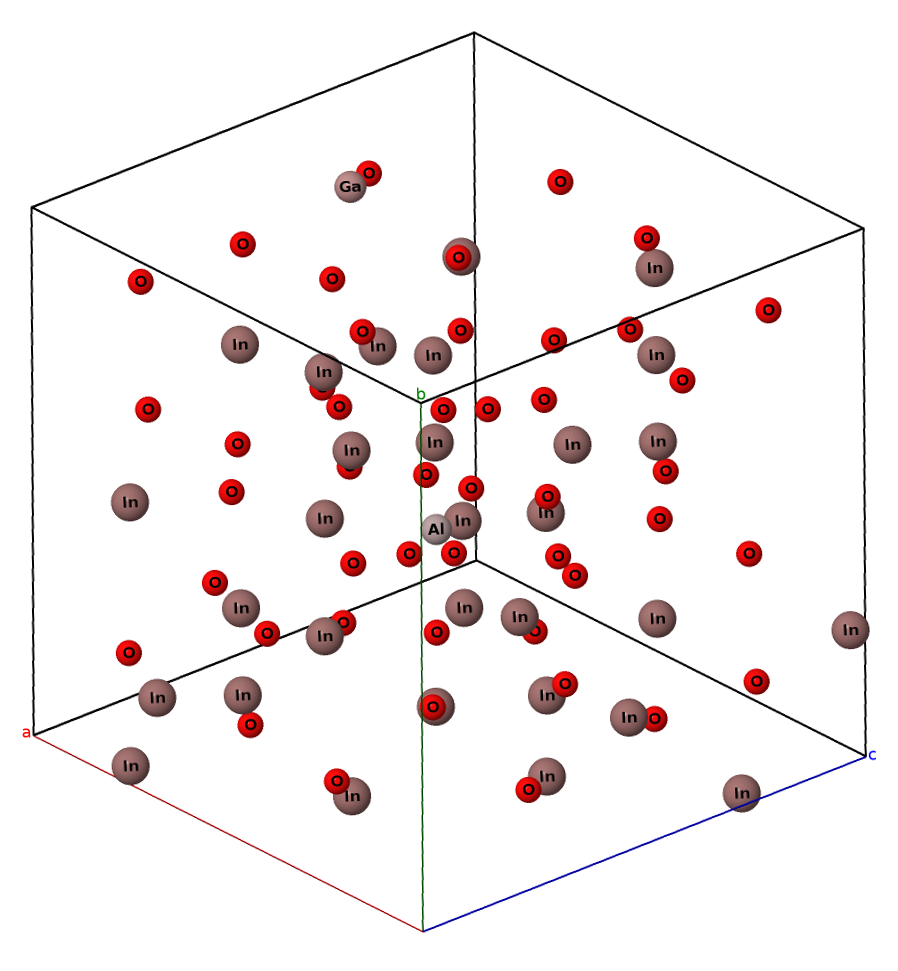
\includegraphics[scale=0.35]{string_label_crop.png}
	\caption{Example of unit cell and atoms. There are 80 atoms in the unit cell: 48 oxygens (red), 30 indiums (brown), 1 aluminium (grey) and 1 gallium (pink). The unit cell is outlined by the three lattice vectors \parencite{jmol}}
	\label{alloy}
\end{figure}
For every crystalline material, there is a set of invariant transformation - a symmetry group - which is called space group and it completely describes the symmetry of the crystal. There are 230 possible space groups for crystalline materials. Interestingly, there are no known crystals for 80 space group and we can choose about 30 most common and important ones which represent the vast majority of the known crystals \parencite{kraus16}.
\subsection{Coordination Numbers and Ionic Radii} \label{numbers_radii}
In the context of a crystal with positively charged atoms (cations) and negatively charged atoms (anions), the amount of ions with opposite charge closest to the given atom is called the coordination number and the geometric shape constructed from the connections of centers of these atoms is called the coordination geometry. It is possible to have many different coordination geometries for a given coordination number. For coordination number equal to 4, the coordination geometry can be tetrahedron or square, for coordination number equal to 6, octahedron, trigonal prism, etc. The free space among the atoms decreases with higher coordination numbers \parencite{kraus16}.

Ionic radius is the idealized state of an cation or anion where we assume a rigid boundary of the ion based on its charge. Shannon also assumes the ionic radius changes with the coordination number. The Shannon ionic radii are calculated and tabulated values. We report the values used in the the Nomad2018 Predicting Transparent Conductors Kaggle competition (coordination VI for metals and coordination II for oxygen) which were calculated by Shannon \parencite{shannon76}.  All Shannon's values for the four elements making up the studied crystals are in Table \ref{shannon_radii}.

\begin{table}[H]
	\centering
	\begin{tabular}{lllll} 
		\hline
		In \AA & $Al^{3+}$    & $Ga^{3+}$    & $In^{3+}$    & $O^{2-}$    \\ 
		\hline
		II     & - & - & - & 1.35  \\
		
		III     & - & - & - & 1.36  \\ 
		
		IV     & 0.39 & 0.47 & 0.62 & 1.38  \\ 
		
		V   & 0.48 & 0.55 & - & -  \\ 
		
		VI   & 0.535 & 0.62 & 0.8 & 1.4  \\ 
		
		VIII   & - & - & 0.92 & 1.42  \\
		\hline
	\end{tabular}
	
	\caption{Shannon ionic radii (in \AA) as reported in \parencite{shannon76} varying with coordination number for the cations of Al, Ga, In and the anion of O}
	\label{shannon_radii}
\end{table}

%Shannon makes the assumption that ionic radii vary with coordination number. This is troubling


\section{Material Descriptors}
The following text explains the ideas of feature engineering used in our application.
\subsection{General Properties} \label{gen}
A descriptor (or a feature) is a representation of the material data with a single vector of numbers. For every material, we denote $q_1, q_2, \dots, q_M \in \mathbb{R}^N, M \in \mathbb{N}$. In the field of application of machine learning in solid state physics, we deal with the task of finding the proper system of descriptors. This singular vector can be given by concatenation of the $M$ vectors into one. %Numerous methods have been used and developed to tackle this problem. The LASSO has proven to be a useful tool for screening moderately sized feature spaces for the most influential descriptors \parencite{ghiringhelli15} and consequently the SISSO method was developed which can screen huge feature spaces \parencite{ouyang18}. %which is more robust than LASSO and has been used with success recently because of its ability to deal with correlated features and huge feature spaces \parencite{DALSI SISSO VECI}.
One of the problems with material descriptors comes when it is needed to use the positional data of the atoms in the molecule or lattice. Cartesian positions are not invariant to rotation and translation of the compound. Additionally, the descriptor should be invariant to swapping two atoms of the same species, in other words, we demand invariance to permutation of atoms of the same species. Lastly, reflectional invariance is also desired. The descriptor should not lose much of the information encoded in the Cartesian coordinates as well. A system of descriptors ${q_1, q_2, \dots, q_M}, M \in \mathbb{N}$ is called complete if and only if there exists a bijective function between the system ${q_1, q_2, \dots, q_M}$ and corresponding Cartesian coordinates. A system of descriptors ${q_1, q_2, \dots, q_M}, M \in \mathbb{N}$ is called over-complete if there is a subset of ${q_1, q_2, \dots, q_M}$ which is complete \parencite{bartok13}. The bijective property of the descriptor is very strong and it can be easier not to enforce it when choosing a material descriptor. Even though the descriptor breaks the bijective property for some crystals it can be bijective so often it does not pose a serious issue. Of course, one can demand additional properties. One of problems with defining a descriptor is the fact that the number of atoms in the unit cell varies a lot and many descriptors are not defined to have a fixed length. Naturally, the problem with assembling these descriptor into a matrix is that either the vectors in the matrix have to be padded or cropped.

Material descriptors which are not based on Cartesian coordinate system are usually quantities describing the species (atomic number, electronegativity, atomic radius, etc.) of the compound or their state (ionic radius, coordination number, charge, etc.). The choice of proper descriptors is determined by the physical feature of the crystal we wish to predict. 
%Interestingly, choosing more quantities as descriptors could make the prediction better in regards to computational data but can decrease the agreement with experimental data \parencite{li19}.

\subsection{Brief Overview of Already Developed Descriptors} \label{developed}
In recent years, many material descriptors have been proposed. We choose to briefly list only a few relevant ones which inspired some of the propositions outlined in the upcoming text below. We also note that many descriptors listed below are designed to work with molecules rather than solids. However, this does not take from the value and inspiration they offer because some of the descriptors can be generalized to be used with crystals but performance of such descriptors can vary greatly.

The early Coulomb matrix representation \parencite{rupp12} has had a great impact on the chemoinformatics community and has been improved upon many times in later publications. For a molecule with $N$ atoms we construct a matrix with entries
\begin{equation}
	\bm{M}_{ij} =
	\begin{cases}
		0.5 {Z_{i}}^{2.4},\space i = j \\
		\frac{Z_i Z_j}{\|\boldsymbol{R}_i - \boldsymbol{R}_j\|_2}, \space i \neq j \\
	\end{cases}	
	\label{coulomb}
\end{equation}
where $Z_i$ is the atomic number of the $i$th atom, $\|\boldsymbol{R}_i - \boldsymbol{R}_j\|_2$ is the distance of atoms $i$ and $j$ in the $\ell_{2}$ norm. The shape of the descriptor is inspired by the Coulomb repulsion potential which is in the Hamiltonian of the DFT equations used to calculate the data. Because the matrix $\bm{M}$ is symmetric, one can find the eigenvalues and conveniently vectorize them as $\boldsymbol{\lambda} = (\lambda_1, \dots, \lambda_N)$, $\lambda_{i}>\lambda_{i+1}$ for $\forall i \in {1,\dots,N}$ and construct a measure of difference of two materials as 
\begin{equation}
	d(\bm{M}, \bm{M'}) = d(\boldsymbol{\lambda}, \boldsymbol{\lambda}') = \| \boldsymbol{\lambda} - \boldsymbol{\lambda}' \|_2
\end{equation}
where $\boldsymbol{\lambda}$ is the spectrum of $\bm{M}$ ordered in decreasing fashion according to absolute value of the eigenvalues. For molecules with different amount of atoms, the shorter spectrum is appended with zeros to match the length of the longer spectrum. Even though it is a very simple representation, it has shown great success. The sorted spectrum of a matrix elegantly solves the problem of invariance outlined before. However, it has been shown \parencite{hansen13} this compression of information from $\frac{1}{2}(N^2 + N)$ unique numbers to $N$ numbers leads to a big information loss. The eigenvalue representation of the Coulomb matrix also results in loss of bijectivity of the representation \parencite{rup12answer}, \parencite{moussa12question}. 

To solve the problem of information loss, it has been proposed to construct sorted Coulomb matrices where the rows (or columns) are sorted according to their $\ell_{2}$ norm in decreasing fashion. Alternatively, the so called random Coulomb matrices can be constructed and these improvements lead to 4-5 times lower prediction error \parencite{hansen13}. The important conclusion of these results is that the reduction of information of a matrix to its eigenvalues to represent materials is too crude and better representations can be found.

The Coulomb matrix descriptor has been improved into a representation called Bag of Bonds (BoB) \parencite{hansen15} in the following way: the entries of matrix $\bm{M}$ in equation (\ref{coulomb}) are put into bags (groups) based on the two atom species of the $\bm{M}_{ij}$ pair. This way, multiple bags of numbers are created, vectorized and padded with zeros to get vectors of equal sizes across all molecules in the dataset. The elements of the vectors are sorted according to their absolute values and finally, all the vectors are concatenated in arbitrary but consistent order across the whole dataset. This representation is invariant under rotations, translations and permutations of atoms of the same species. Also, it conveniently vectorizes the descriptor however, the padding with zeros procedure reduces the elegance of this approach. The further introduction of atomic species into the descriptor building procedure is a valuable idea and will play central role in the follow sections.

The attempts to extended the Coulomb matrix approach to crystalline materials have not performed well \parencite{faber15}. 

Ionic radii and functions of ionic radii appear to be good descriptors for predicting stability of perovskites structures. The accuracy of the prediction of the same regression problem was attempted to be improved by adding electronegativities of the species as another descriptor. This lead to some increase in prediction accuracy but the unexpected cost was much worse agreement of the prediction with laboratory experiments \parencite{li19}. This is in accordance with the principle of Occam's razor - we want to choose the simplest model possible which explains the phenomenon. Also, such models possess much better interpretability and we can learn more easily from their behavior about the problem we are solving.

Recently, crystal graph multilayer descriptor (CGMD) was used to predict properties of 2D materials \parencite{lu20} and utilizes the adjacency matrix of a crystal graph for solids. This is outlined in \parencite{xie18}. One of the caveats of this representation is that the descriptor length depends on the size of the structure it describes.

% Smooth Overlap of Atomic Positions (SOAP) \parencite{bartok13}, \parencite{bartok15} which placed 3rd in the Nomad2018 Predicting Transparent Conductors Kaggle competition \parencite{sutton18}, \parencite{sutton19}
Among other descriptors reviewed belong the many-body tensor representation (MBTR) which works for both molecules and crystals and extends the Coulomb matrix and Bag of Bonds approaches \parencite{huo17}, partial radial distribution function (PRDF) representation for crystals \parencite{schutt14}, and the crystal graph of \parencite{xie18}.
\subsection{Studied Descriptors}
The following text dives deeper into the structure of two descriptors which are ngram and Smooth Overlap of Atomic Positions (SOAP). Eventually, proposals of improvement of these descriptors are made based on the knowledge gathered about the physical problem and the available data.
\subsubsection{ngram}
The  ngram representation won the Nomad2018 Predicting Transparent Conductors Kaggle competition which was studied \parencite{sutton18}, \parencite{sutton19}, \parencite{kaggle_web}. For the purposes of the crystal graph representation of crystalline materials, we introduce additional quantities which build upon the text of Section \ref{physical}.

The positions itself of the atoms in the unit cell introduced in Section \ref{physical} do not possess enough information for the construction of a meaningful representation for solids. Considering periodicity of the unit cell, we start by defining the reduced distance between atoms $i$ and $j$ (using the knowledge from Section \ref{reducedhere}) as
\begin{equation}
	\bm{r}^{k,l,m}_{ij} = \bm{r}_i - \bm{r}_j + (k, l, m)^T,    k,l,m \in \mathbb{Z}.
\end{equation}

The conversion to actual physical distance is given by

\begin{equation}
	\bm{R}^{k,l,m}_{ij} = \bm{A} \bm{r}^{k,l,m}_{ij}.
\end{equation}

Finally, the spatial distance of two atoms $i$ and $j$ over all possible neighboring cells is

\begin{equation}
	d_{ij} = \min_{k,l,m \in \mathbb{Z}}{\|\bm{R}^{k,l,m}_{ij}\|_2}.
\end{equation}

Therefore, we introduce the distance matrix as the closest distances between two atoms over all possible unit cells

\begin{equation}
	\bm{D}_{ij} = 
	\begin{cases}
		0,\space i = j \\
		d_{ij}, \space i \neq j.
	\end{cases}
\end{equation}

As outlined in Section \ref{numbers_radii}, the coordination number and coordination geometry considers only pairs of atoms where one is negatively charged and the other positively (for our dataset it means that for oxygen only the connections with the three metals are considered and vice versa). We collect the count of the amount of neighbors of each atom using the following rule

\begin{equation}
	\bm{D}_{ij} < \alpha (R^{S}_i + R^{S}_j).
	\label{decision}
\end{equation}

If the inequality above holds, then atom $i$ is in the coordination environment of $j$ and vice versa. The number $\alpha$ is determined beforehand and depends on the space group of the material. The value is chosen so that the amount of coordination atoms of each atom is roughly similar to actual physical coordination of such geometric configuration of the atoms. We enforce more physical meaning this way into the descriptor because the distribution of coordinations with these numbers is very physical and limits spurious behavior of the ngram descriptor.

\begin{table}[H]
	\centering
	\begin{tabular}{cccccccccc} 
		\hline
		&  12   &  33    & 167    & 194 & 206 & 227 ($\gamma<60^{\circ}$) & 227 ($\gamma \geq 60^{\circ}$)   \\ 
		\hline
		$\alpha$  & 1.4 & 1.4 & 1.5 & 1.3 & 1.5 & 1.4 & 1.5  \\ 
		\hline
	\end{tabular}
	\caption{The value of $\alpha$ depends on the space group, $\gamma$ is the angle between lattice vectors $\bm{a}$ and $\bm{b}$}
	\label{alpha}
\end{table}
An atom X with $n \in \mathbb{N}$ of coordination atoms is referred to as X-n. For example, aluminum with 4 oxygens in its coordination environment is called Al-4. The number of atoms with the same coordination numbers is calculated, the values are divided by the volume of the unit cell $V_{cell}$ because the cell sizes differ for every space group and the lattice vectors of Bravais lattice are not given unambiguously\footnote{for example, the length of every lattice vector can be two times bigger and consequently, the unit cell would include 8 times bigger volume with more atoms. This way, the counts of atoms of given coordination are normalized} and a histogram of these values is created. This representation is the unigram. The same principle works for counting chains of various length of particular atom-coordination pairs. We can count the number of normalized atom-coordination pairs, denoted X-n/Y-m (for example Al-4/O-3). It is easy to see that X-n/Y-m and Y-m/X-n have the same meaning. This representation is called the bigram. We can go further and count numbers of normalized triples (trigram), denoted X-n/Y-m/Z-l. Obviously we can go even further and construct quadgrams etc. Collectively, we call these representations ngrams. The ngram representation combined with kernel ridge regression won the Nomad2018 Predicting Transparent Conductors Kaggle competition \parencite{sutton18}, \parencite{sutton19}.

The representation can be viewed as an extension of the concept of percentages of different atoms in the compound.
It is important to note that the coordination numbers and geometries which can be obtained from relaxed calculations or not fully converged calculations are not strictly within the crystallographic rules (e. g. symmetries can be broken because of the numerical nature of the result from the DFT software calculation). However, this does not take anything from the physical interpretability and performance of this representations.

In practice, the amount of X-n atom-coordination pairs is determined by the dataset. In general, the amount of columns of the regressor matrix of is $kc$ for unigram, $\binom{kc}{2}$ for bigram, $\binom{kc}{3}$ for trigram and so on, where $k$ is the amount of atom species in the whole dataset and $c$ is the amount of coordinations running from 0 to $c$-$1$. The ngram can get very cumbersome for datasets with many atomic species however it turns out many columns are completely empty for trigram and quadgram. This sparsity is heavily influenced by the dataset we have. Our dataset has only 6 spacegroups and 4 atoms in it. A dataset with more spacegroups and more atoms would promote much lower sparsity.

This descriptor is invariant to rotations, translations, reflections and permutations of atom of the same species. 

\subsubsection{ngram Extended}
We propose to extend the ngram representation to include in some sense the physical distances of the atoms in the coordination environment of every atom. We start with the atom-coordination information constructed previously and for an atom X with coordination $n$ denoted as a pair X-n we introduce

\begin{equation}
	\Sigma_{\text{X-n}}(p) =
	\begin{cases}
		\|\text{X-n}\|, p=0, \\
		\frac{1}{\|\text{X-n}\|}\sum_{i}^{|\text{X-n}|} \bm{D}_{iX}^p, p \neq 0, \\
		%\Sigma^{R^S}_{\text{X-n}}(p) = \frac{1}{\|\text{X-n}\|}\sum_{i}^{|\text{X-n}|} \Bigg(\frac{\bm{D}_{ij}}{R^S_i}\Bigg)^p
		
	\end{cases}
\label{proposed}
\end{equation}
and a scaled version where the distances between atoms are scaled by the Shannon ionic radius (Table \ref{shannon_radii}) of the central atom of the coordination environment (radius of coordination II is used for oxygen and VI is used for metals) as

\begin{equation}
	\tilde{\Sigma}_{\text{X-n}}(p) =
	\begin{cases}
		\|\text{X-n}\|, p=0, \\
		\frac{1}{\|\text{X-n}\|}\sum_{i}^{|\text{X-n}|} \frac{\bm{D}_{iX}^p}{R^S_X}, p \neq 0, \\
		%\Sigma^{R^S}_{\text{X-n}}(p) = \frac{1}{\|\text{X-n}\|}\sum_{i}^{|\text{X-n}|} \Bigg(\frac{\bm{D}_{ij}}{R^S_i}\Bigg)^p
		
	\end{cases}
	\label{proposed}
\end{equation}
where $|\text{X-n}|$ symbolizes all the atoms of the coordination environments of all atoms which are X-n and $||\text{X-n}||$ symbolizes the total amount of atoms in the coordination environments of all X-n atoms. Number $p \in \mathbb{Z}$ manages further extension of the descriptor where the most interesting are $p=1$ which gives the first sum the meaning of average distance of the atoms of the coordination environment which can also be interpreted as the average bond distance of metal atoms from oxygen atoms. The choice $p=-1$ possesses information similar to the Coulomb matrix descriptor from Section \ref{developed}. The choice $p = 0$ gives the amount of neighboring atoms. A physical meaning of terms for $p=-6$ and $p=-12$ can be found in the structure of a well-known Lennard-Jones potential for classical modeling of atomic interactions \parencite{wang20}
\begin{equation}
	\nu_{LJ}(r) = 4\epsilon \Bigg( \Big[ \frac{\sigma}{r} \Big]^{12} - \Big[ \frac{\sigma}{r} \Big]^6 \Bigg),
	\label{lj}
\end{equation}
where $\epsilon$ is a constant describing the depth of a potential energy well, $r$ is the interatomic distance and $\sigma$ is the interparticle distance where the Lennard-Jones potential changes sign and this change describes the change between repulsive and attractive nature of the potential. Our descriptor therefore attempts to model in some sense the $r^{-6}$ and $r^{-12}$ terms which the developed physical understanding of the problem showed to bring good description of the problem of crystalline stability.
 Other values of $p$ do not necessarily have a direct physical meaning but one can view them as a part of the expansion into Laurent series or an attempt to take into account higher order interactions similar to the LASSO experiment in Chapter 3.

The physical interpretation of this descriptor comes from the assumption that all atoms of the same species and the same coordination have roughly the same coordination environment in terms of distances and species. The repulsing or attracting significance (in the context of (\ref{lj})) of the term in the sum of $\Sigma_{\text{X-n}}(p)$ or $\tilde{\Sigma}_{\text{X-n}}(p)$ is determined by the coefficient in the kernel ridge regression model. This extension of ngram is also invariant to rotations, translations, reflections and permutations of atoms of the same species but as can be easily seen from the construction (taking the average of distances), it is not bijective to the Cartesian coordinate system.

The procedure of ngram and extended ngram construction outlined above is applied to $(Al_{0.25}Ga_{0.25}In_{0.5})_2 O_3$ alloy as an example which can be found in Appendix B.
\begin{figure}[H]
	\centering
	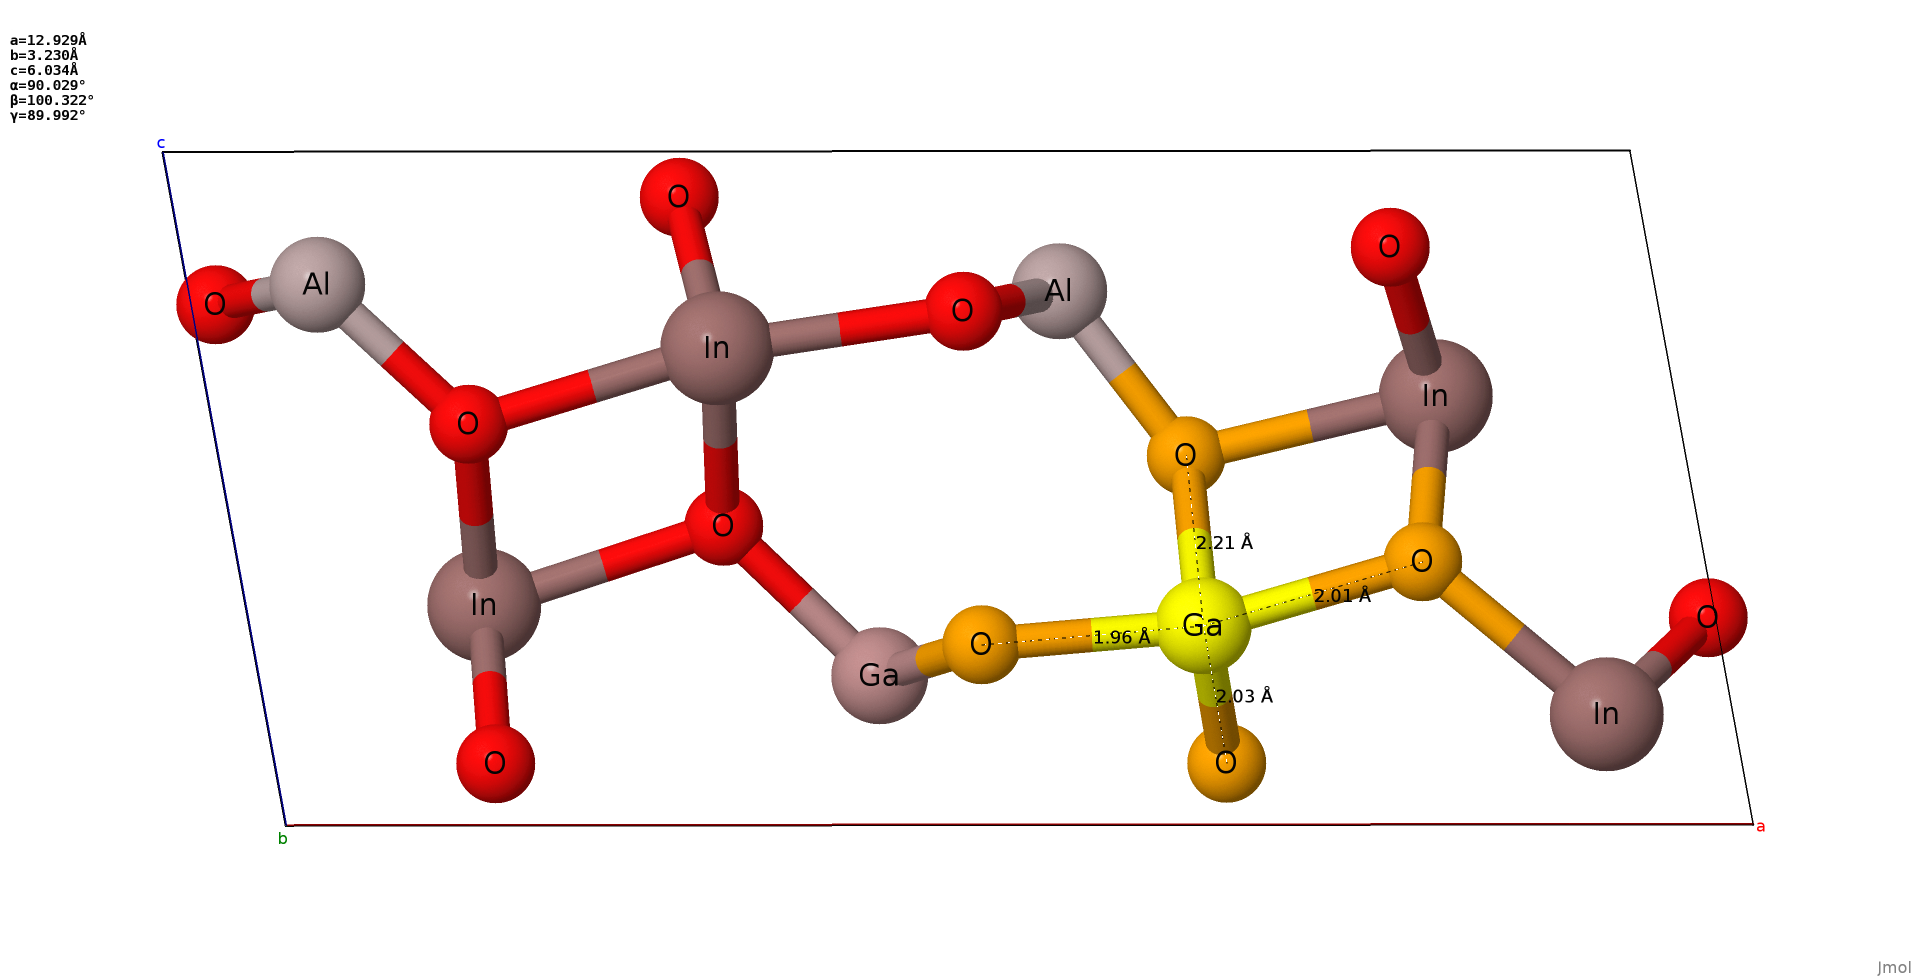
\includegraphics[scale=0.23]{train_id_20_final_Ga4_hotovo.png}
	\caption{Alloy $(Al_{0.25}Ga_{0.25}In_{0.5})_2 O_3$ with one atom of gallium in yellow and its coordination environment in orange with the interatomic distances (notice the distances are approximately 2 $\text{\AA}$). This gallium atom has 4 oxygens in its coordination environment, therefore it is Ga-4. The other gallium atom of the alloy is Ga-3 where the third oxygen atom is not displayed because it is in the neighboring unit cell. Still, it is close enough to fulfill the condition in equation (\ref{decision}) \parencite{jmol}}
\end{figure}

\subsubsection{Smooth Overlap of Atomic Positions (SOAP)}
The SOAP representation placed 3rd in the Nomad2018 Predicting Transparent Conductors Kaggle competition which was studied \parencite{sutton18}, \parencite{sutton19}, \parencite{kaggle_web}. For the purposes of developing the SOAP representation, we define the neighbor density function of an atom X as
\begin{equation}
	\rho(\bm{r}) = \sum_{i} w_{X} \delta(\bm{r}-\bm{r}_i),
\end{equation}
where we sum over all the atoms in the atomic neighborhood of an atom which is defined with some cutoff distance from the central atom, $w_{X}$ is a weighing factor of an atom based on its species and $\bm{r} - \bm{r}_i$ is the vector from the central atom X to the atom $i$.

%\subsubsection{SOAP Extended}

\chapter{Classification Problem of Binary Compounds Experiment}
The goal of this experiment is to develop a model for prediction of the crystal structure of semiconductors. These compounds are simple: binary compounds AB consisting of element A and element B. The dataset consists of compounds which crystallize in three distinct structures: rocksalt (RS), zincblende (ZB) and wurtzite (WZ). Figure \ref{jmol_struct} shows the geometry of the aforementioned structures. However, the energies of ZB and WZ are very close (see Appendix A, column $E(ZB) - E(WZ)$) and for the sake of simplicity, these two structures are not distinguished in this experiment (the corresponding $\Delta E_{WZ}$ for the dataset is in a table in Appendix A). The target property of this experiment is the difference between the energy of rocksalt $E_{RS}$ and the energy of zincblende $E_{ZB}$ for the given compound AB - that is $\Delta E = E_{RS} - E_{ZB}$. Therefore, our goal is to find a model for binary compounds AB which assigns them the right crystalline structure - the sign of the energy difference $\Delta E_{AB}$ gives the structure.

\begin{figure}[H]       
	%\fbox{}   
	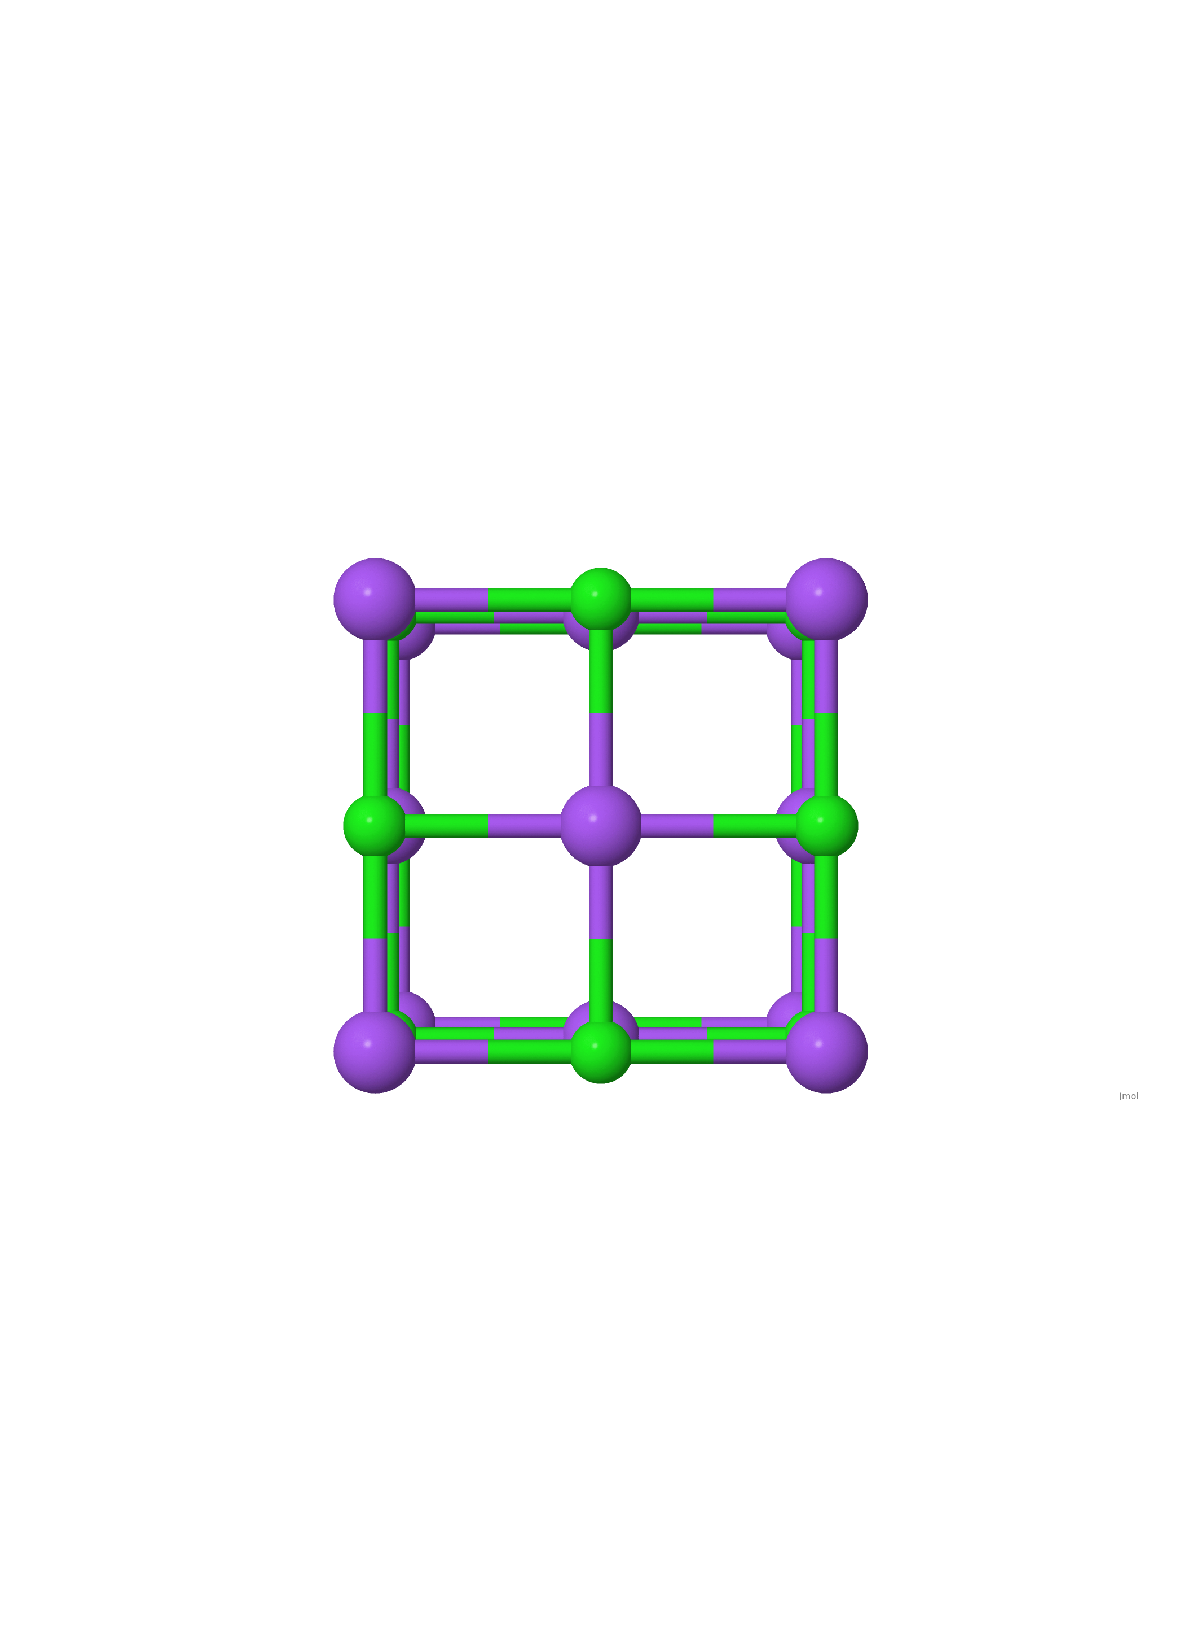
\includegraphics[scale=0.26]{rocksalt_nolabels.pdf}
	%\hspace{30px}
	%\fbox{}
	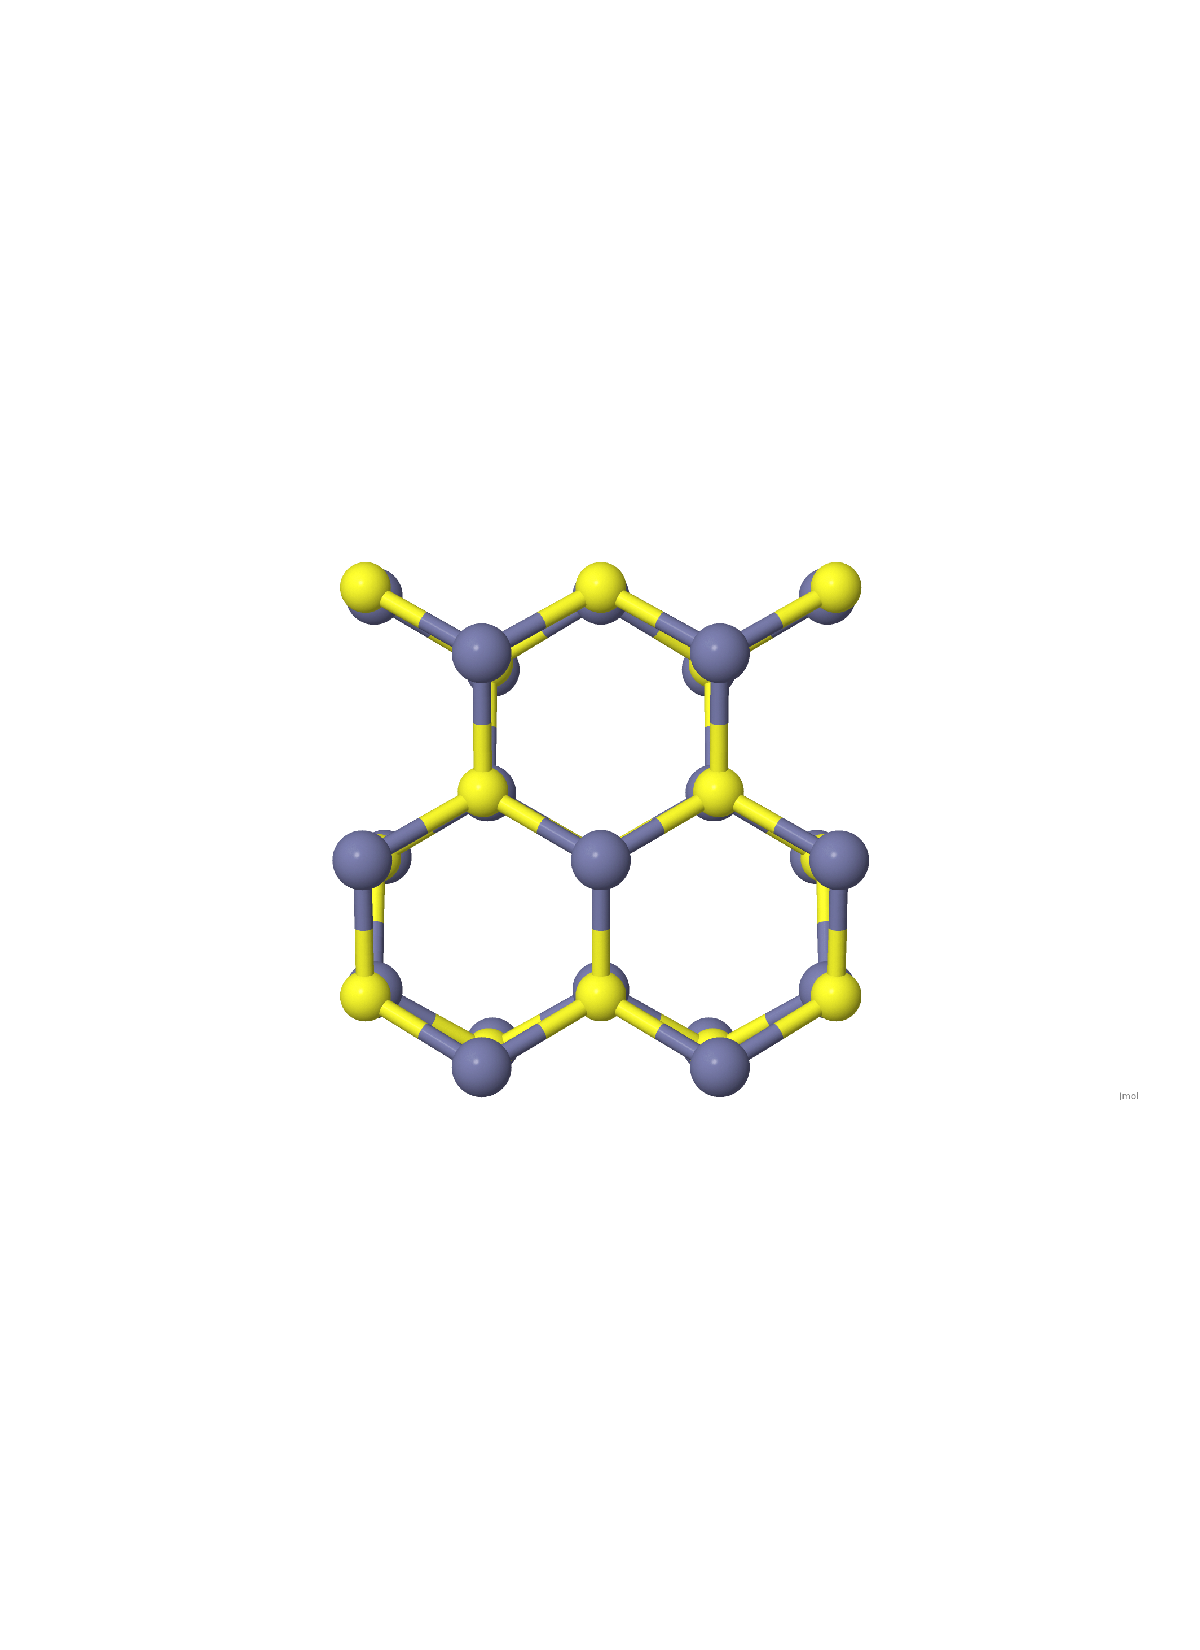
\includegraphics[scale=0.26]{wurtzite_nolabels.pdf}
	%\hspace{30px}
	%\fbox{}
	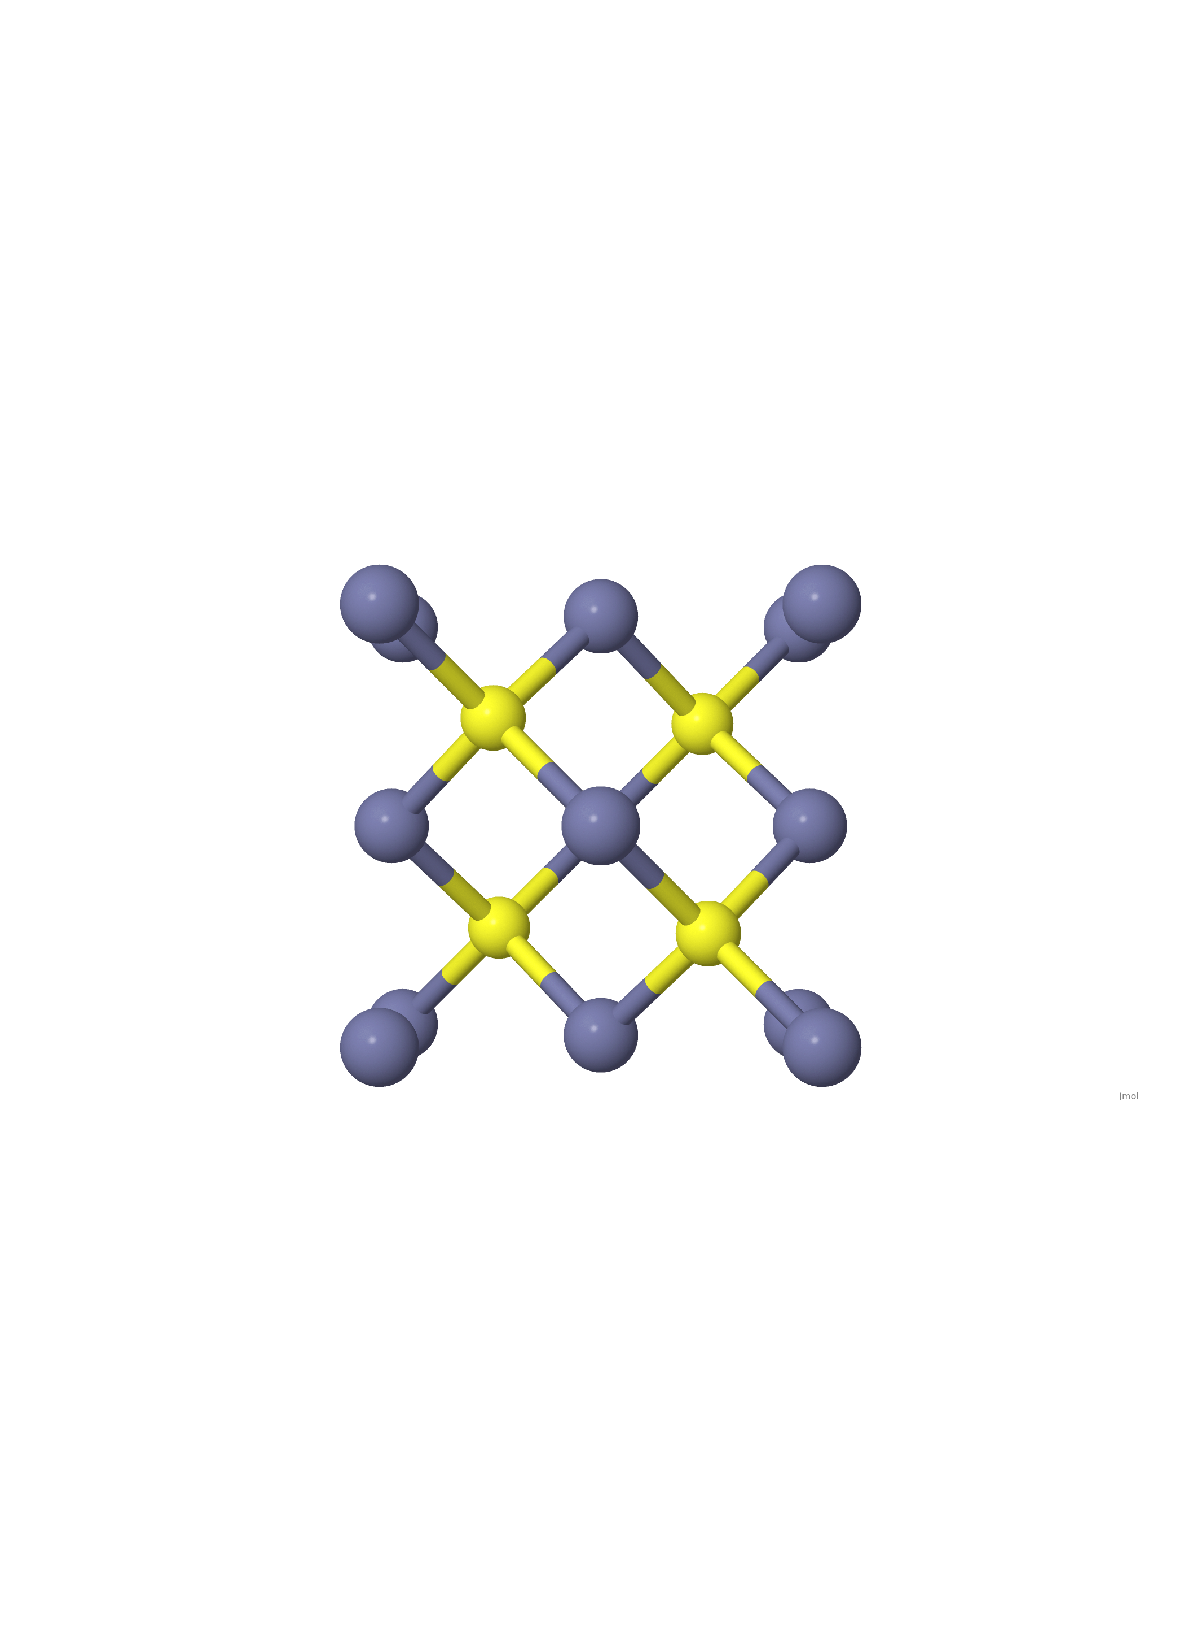
\includegraphics[scale=0.26]{zincblende_nolabels.pdf}
	\caption{From left to right: rocksalt, wurtzite and zincblende structures \parencite{jmol}, \parencite{RS_ZB_WZ}}
	\label{jmol_struct}
\end{figure}

%We demand a reasonable compromise between the time needed to gather the data for modeling and the accuracy of the model. That is, the model should be much less expensive than other means of evaluation of the crystal structure although it could be much less accurate. We will attempt to find low dimensional descriptors to model the energy difference of RS and ZB crystal structures.

\section{The Dataset}
The dataset consists of 34 elements for which 7 physically meaningful features were calculated\footnote{$1\AA = 10^{-10} m$, $1 eV = 1.602 \cdot 10^{-19} J$}:
%\begin{center}

%$\textbf{p}$ =	\Big( \textit{IP} [eV], \textit{EA} [eV], \textit{H} [eV], \textit{L} [eV], $r_{s}$ [Å], $r_{p}$ [Å], $r_{d}$ [Å] \Big),
%\end{center}

\begin{itemize}
	\item Ionization potential IP [eV]
	\item Electron Affinity EA [eV]
	\item Highest Occupied Molecular Orbital H [eV]
	\item Lowest Unoccupied Atomic Orbital L [eV]
	\item Radius where Radial Probability Density of valence \textit{s} orbital is maximal $r_{s}$ [Å] 
	\item Radius where Radial Probability Density of valence \textit{p} orbital is maximal $r_{p}$ [Å] 
	\item Radius where Radial Probability Density of valence \textit{d} orbital is maximal $r_{d}$ [Å] 
\end{itemize}
In total 82 datapoints are available in this dataset (the table with the used data is available in Appendix A). The combinations of the 34 elements into 82 compounds models actual materials which exists in nature which means they are not picked arbitrarily. It is only natural to do such a constraint because we want to predict actual natural phenomena.
It comes from quantum mechanics that the physical features are correlated in terms of the Pearson correlation coefficient of two 82-dimensional feature vectors. The physical meaning of the differences {H-L} and {IP-EA} is very similar. The radii are correlated with the energy quantities as well. The correlation of the features is an issue and it will come up later on during the conducted experiments.

For the 82 compounds, the energy difference $\Delta E = E(RS) - E(ZB)$ was calculated. We put $\vec{y}$ = $\vec{\Delta E}$ in accord with the notation used previously. The labelling AB is not arbitrary. The label A is assigned to the element with lower Mulliken Electronegativity given by $EN = - \frac{1}{2} (EA+IP)$. This way, 14 primary features of a compound AB are defined as

\begin{equation}
	\bm{x}_{AB} = \Big(IP(A), EA(A), H(A), L(A), r_s(A), r_p(A), r_d(A), IP(B), EA(B), H(B), L(B), r_s(B), r_p(B), r_d(B)\Big).
	\label{primary_vector}
\end{equation}
%dim\big(\Phi(\textbf{x}_{AB})\big)
\subsection{The Feature Space Generation}
To capture the relationship between the variables in (\ref{primary_vector}), a nonlinear mapping $\Phi: \mathbb{R}^{14} \rightarrow \mathbb{R}^{M}$ is defined together with a set of unary and binary operations
\begin{equation}
	\big\{|-|, +, /, \cdot, ()^2, \exp[]\big\},
	\label{operations}
\end{equation}
  that execute the mapping and the primary features $\textbf{x}_{AB}$ are used to generate a feature space of expressions from which the matrix $\vec{X}$ is constructed. The operations defined in (\ref{operations}) are (in order of appearance) difference with absolute value, summation, multiplication, power of two and exponential.
  
   From this high dimensional matrix $\bm{X}$, the optimal descriptors (features) will be chosen. The mapping procedure introduces non-linearity needed for better description of the relationship between the primary features in (\ref{primary}) and the energy difference $\Delta E_{AB}$.% Then the regression methods are applied on this large set of expressions.

We will use the inequality (\ref{divnanerovnost}) which gives the estimate that roughly a few thousand features are admissible for our amount of measurements. The primary features are divided into subsets based on their physical units and meaning for more convenient illustration of the generation procedure.
\begin{table}[H]
	\centering
	\begin{tabular}{lll} 
		\hline
		ID & Quantities~ ~                                                                                        & Set size  \\ 
		\hline
		A1 & $IP(A), EA(A), IP(B), EA(B)     $                                                                      & 4   \\ 
		
		A2 & $H(A), L(A), H(B), L(B) $                                                                              & 4   \\ 
		
		A3 & $r_{s}(A)$, $r_{p}(A)$, $r_{d}(A)$, $r_{s}(B)$, $r_{p}(B)$, $r_{d}(B)$ & 6   \\
		\hline
	\end{tabular}
	\caption{The primary features divided into subsets based on their units and meaning}
	\label{primary}
\end{table}
The features in (\ref{primary}) are then combined as follows and their number is calculated:
\begin{itemize}
	\item B1: The sum and the absolute difference of two different features from A1
	\item B2: The sum and the absolute difference of different two features from A2
	\item B3: The sum and the absolute difference of two different features from A3
	\item C3: Squares of all A3 features and squares of all sums of features in B3
	\item D3: Exponentials of all A3 features and all sums in B3
	\item E3: Exponentials of C3
	\item F1: The following 4 expressions:
	
	\begin{center}
		$\big||IP(A)-EA(A)|+|IP(B)-EA(B)|\big| \newline
		\big||IP(A)-EA(A)|-|IP(B)-EA(B)|\big| \newline
		\big||IP(A)+EA(A)|+|IP(B)+EA(B)|\big| \newline
		\big||IP(A)+EA(A)|-|IP(B)+EA(B)|\big| \newline$
	\end{center}
	\item F2: The following 4 expressions:
	
	\begin{center}
		$\big||H(A)-L(A)|+|H(B)-L(B)|\big| \newline
		\big||H(A)-L(A)|-|H(B)-L(B)|\big| \newline
		\big||H(A)+L(A)|+|H(B)+L(B)|\big| \newline
		\big||H(A)+L(A)|-|H(B)+L(B)|\big| \newline$
	\end{center}
	\item F3: The same 4 expressions as in F1, F2 with inputs of all pairs of $r_{s}(A)$, $r_{p}(A)$, $r_{d}(A)$ in the first absolute term and all pairs of $r_{s}(B)$, $r_{p}(B)$, $r_{d}(B)$ in the second term
	
	\item G: Ratios of all expressions in \{Ai, Bi\} with all expressions in \{A3, C3, D3, E3\} for i = 1, 2. The ratio 1/A3. Ratios A3/A3, A3/C3, B3/A3, B3/C3 such that only the unique expressions are chosen
\end{itemize}

This gives total of 4376 potential descriptors and therefore 4376 columns of $\vec{X}$ which comfortably fits the estimate. The number of descriptors and examples for each set are given in Table \ref{descriptors}.

\begin{table}[h]
	\centering
	\begin{tabular}{clc}
		\hline
		ID & Feature examples~ ~                                                                                        & Set size  \\
		\hline
		&&\\ [-1em]
		B1 & $|IP(A)+IP(B)|$, $|IP(B) - EA(B)|$, ...                                                                      & $2\binom{4}{2} = 12$   \\
		
		&&\\ [-1em]
		B2 & $|H(A)+H(B)|$, $|H(B) - L(B)|$, ...                                                                                      & $2\binom{4}{2} = 12$   \\
		
		&&\\ [-1em]
		B3 & $|r_s(A) - r_p(A)|$, $\big(r_d(B) + r_s(A)\big)$, ... & $2\binom{6}{2} = 30$  \\
		
		&&\\ [-1em]
		C3 & $r_s(A)^2$, $\big(r_d(B) + r_s(A)\big)^2$, ...                                                                      & $6+\binom{6}{2}=21$   \\
		
		&&\\ [-1em]
		D3 & $\exp\big[r_s(A)\big]$, $ \exp\big[r_d(B) + r_s(A)\big]$, ...                                                                      & $6+\binom{6}{2}=21$   \\
		
		&&\\ [-1em]
		E3 & $\exp\big[r_s(A)^2\big]$, $\exp\big[\big(r_d(B) + r_s(A)\big)^2 \big]$, ...                                                                      & $6+\binom{6}{2}=21$   \\
		
		&&\\ [-1em]
		F1 & $\big||IP(A)-EA(A)|+|IP(B)-EA(B)|\big|$, ...                                                                      & $4$   \\ 
		
		&&\\ [-1em]
		F2 & $\big||H(A)-L(A)|+|H(B)-L(B)|\big|$, ...                                                                      & $4$   \\ 
		
		&&\\ [-1em]
		F3 & $\big||r_s(A)-r_p(A)|+|r_s(B)-r_p(B)|\big|$, ...                                                                      & $36$   \\
		
		&&\\ [-1em]
		G & $\frac{IP(A)}{r_s(A)}$,$\frac{IP(A)}{(r_p(A)+r_s(B))^2}$, $\frac{IP(A)}{\exp\big[r_s(A)\big]}$, $\frac{|r_p(A)-r_s(B)|}{\exp\big[r_p(B)\big]}$, ...                                                                      & $4201$   \\
		\hline
	\end{tabular}
	\caption{Application of the chosen operations on primary features and the corresponding set sizes}
	\label{descriptors}
\end{table}
The feature space used in this work is almost the same as the one in \parencite{ghiringhelli17}.

\subsection{The LASSO+$\ell_{0}$ Method}
It was briefly noted earlier in this chapter that the correlation of the features is an issue. Additionally, we use combinations of already correlated quantities and therefore we can expect the correlation of the generated features to be a problem as well. Indeed, as it turns out LASSO itself performs unpredictably for values of $\lambda$ which choose 1D, 2D, 3D and 4D descriptors and the optimal descriptor cannot be chosen this way reliably as we would do so for columns of a matrix with low correlation (see Table \ref{instability}).

\begin{table}[H]
	\centering
	\begin{tabular}{lll} 
		\hline
		$\lambda$ value & Column index                                                                \\ 
		\hline
		$\lambda_1$ = 0.4229    & None                                                               \\ 
		
		$\lambda_2$ = 0.3944    & 819                                                         \\ 
		
		$\lambda_3$ = 0.3679    & 819, 1105                                                  \\ 
		
		$\lambda_4$ = 0.3431    & 819, 1105, 1470                                             \\ 
		
		$\lambda_5$ = 0.3199    & 819, 1105, 1470, 2172                                        \\ 
		
		$\lambda_8$  = 0.2595    & 819, 1105, 1470, 2172, 966                                  \\ 
		
		$\lambda_{10}$ = 0.2257    & 819, 1105, 1470, 2172, 966, 903, 1021                             \\ 
		
		$\lambda_{12}$ = 0.1963    & 819, 1105, 1470, 2172, 903, 1021, 966                       \\ 
		
		$\lambda_{14}$ = 0.1707    & 1105, 819, 1470, 2172, 903, 1021, 2540, 966                \\ 
		
		$\lambda_{15}$  = 0.1592    & 1105, 819, 1470, 2172, 1021, 903, 2540        \\ 
		
		$\vdots$  & $\vdots$                                                   \\ 
		
		$\lambda_{72}$ = 0.003     & 3441, 2562, 1259, 4125, 4270, 3013, 2235, 2561, ...         \\
		\hline
	\end{tabular}
	\caption{Found descriptors for given $\lambda$ value sorted from the most significant to the least significant}
	\label{instability}
\end{table}

The $\lambda_i$ value is chosen using the following recursive formula

\begin{equation}
	\lambda_i = {\Bigg(\frac{1}{1000}\Bigg)}^{dim(\lambda)-1} \lambda_{i-1}, i \in \{2, \dots, dim(\lambda)\}
\end{equation}
where $dim(\lambda)$ means the number of $\lambda$ values evaluated during the LASSO+$\ell_{0}$ procedure, $\lambda_1 = \frac{1}{N} \max_{i} | \langle \vec{x}_i , \vec{\Delta E} \rangle|$ is the threshold value when the first non-zero coefficient appears. The vector $\vec{x}_i$ is a column of $\vec{X}$ and $\vec{\Delta E}$ is the vector of energy differences. This formula was derived from the approaches to choosing $\lambda$ values in \parencite{ghiringhelli17}.

The procedure appears to be reasonably stable for $\lambda$ close the threshold $\lambda_1$. The significance of the first descriptor decreases with the descend of $\lambda$ and it completely disappears for certain low values of $\lambda$. The more non-zero coefficients are admissible, the less reliable the LASSO selection appears to be. For $\lambda \approx 0.003$, there are 42 non-zero coefficients and the selection hierarchy is completely different compared to selections with higher $\lambda$ values. Therefore, the following approach has been proposed \parencite{ghiringhelli15}: The LASSO selection is carried out for a beforehand chosen vector of $\lambda$ values with length $dim(\lambda)$. From these LASSO selections for various $\lambda$, the best $\Theta$ ocurring descriptors throughout the calculations are gathered and among
these the best 1D, 2D, 3D and 4D descriptor are found using the least squares regression method for all $\binom{\Theta}{1}, \binom{\Theta}{2}, \binom{\Theta}{3}, \binom{\Theta}{4}$ which is effectively the $\ell_{0}$ minimization. The 1D, 2D, 3D and 4D OLS models with the lowest MSEs are selected as the winners.

%\begin{equation}
%\sqrt{\frac{1}{N}\sum_{j=1}^{N}\big(y_j - \hat{y}_j\big)}^2 = \sqrt{\frac{1}{N}\sum_{j=1}^{N}\big({\Delta E}_j - {\Delta E_{kD}}_j \big)}^2 = \sqrt{\frac{1}{N}\sum_{j=1}^{N}\big({\Delta E}_j - \sum_{i =1}^{k}\tilde{A}_{ji}\hat{x}_i\big)}^2,
%\end{equation}

%where $\tilde{\vec{A}}$ is a matrix $\vec{A}$ narrowed to the given $k$ columns and $\vec{\hat{x}}$ is the least squares vector of coefficients calculated with $\vec{\tilde{A}}$ and $\vec{y} = \vec{\Delta E}$ as input in (\ref{least_squares}) for $k \in \{1,2,3,4\}$. 
%The model with the lowest RMSE is selected. The reason to use root mean squared error instead of mean squared error is that the unit of RMSE is [eV] which corresponds to the unit of the energy difference we want to predict.

%Additional quantity called max residual error (MRE) is also reported
%\begin{equation}
%\max_{j}\big\{| y_j - \hat{y}_j|\big\} = \max_{j}\big\{| {\Delta E}_j - {\Delta E_{kD}}_j \big\} = \max_{j}\big\{ | {\Delta E}_j - \sum_{i =1}^{k}\tilde{A}_{ji}\hat{x}_i |\big\}.
%\end{equation}

The issues and peculiarities of this approach which naturally appeared will be discussed thoroughly in the following text.

%It is not a priori clear how many values of $\lambda$ are needed to gather enough descriptors or how big we should choose the $\Theta$ parameter. 

\subsection{Results and Discussion}
The setting was chosen to be $dim(\lambda)=100$ values of $\lambda$ starting from the threshold $\lambda_1$ and decreasing as a geometric sequence with $\lambda_{100} \approx 4.23 \cdot 10^{-4}$ being the lowest. The amount of contending descriptors was set to be $\Theta = 30$. This choice will be discussed later on further. Before the training, the data were standardized and the sci-kit learn \parencite{scikit-learn} LASSO implementation was used.

The LASSO+$\ell_{0}$ method found the following models in the sense of minimal MSE:
\footnotesize
\begin{align}
	\Delta E_{D1} &= 0.055 \frac{|IP(A)+IP(B)|}{r_p(A)^2} -0.332 \label{1D} \\
	\Delta E_{D2} &= 0.113 \frac{|IP(B)-EA(B)|}{r_p(A)^2} -1.558 \frac{|r_s(A)-r_p(B)|}{\exp(r_s(A))} -0.133 \label{2D} \\
	\Delta E_{D3} &= 0.108 \frac{|IP(B)-EA(B)|}{r_p(A)^2} -1.751\frac{|r_s(A)-r_p(B)|}{\exp(r_s(A))} -9.042\frac{|r_s(B)-r_p(B)|}{\exp(r_d(A)+r_s(B))} -0.027  \label{3D} \\
	\Delta E_{D4} &= 0.186 \frac{|H(A)+H(B)|}{\exp(r_p(A)^2)} -1.031\frac{|r_s(A)-r_p(B)|}{\exp(r_s(A))} - 11.246 \frac{|r_s(B)-r_p(B)|}{\exp(r_d(A)+r_s(B))} + 234.153 \frac{|r_s(A)-r_d(B)|}{\exp[(r_s(A)+r_d(B))^2]} + 0.072 \label{4D}
\end{align}
\normalsize
The starting point is the worst possible RMSE = 0.457 eV which is for prediction $\Delta E_{D_j} = 0$ for $j \in \{1,2,3,4\}$ (the coefficients of the model are zero). Test RMSE and MaxAE of the models are reported in Table \ref{RMSE MRE}.
\begin{table}[h]
	\centering
	\begin{tabular}{lllll} 
		\hline
		In eV & 1D    & 2D    & 3D    & 4D     \\ 
		\hline
		RMSE  & 0.138 & 0.099 & 0.076 & 0.063  \\ 
		MaxAE   & 0.421 & 0.287 & 0.243 & 0.163  \\
		\hline
	\end{tabular}
	\caption{Test RMSE and test MaxAE of the best models}
	\label{RMSE MRE}
\end{table}
The 2D and 3D descriptors match exactly the ones from \parencite{ghiringhelli15}. However, slightly different coefficients were recovered. This is most likely rounding error during the handling of the values and feature space generation. Also, it is possible a different implementation of the numerical solver was used which can result in slight inaccuracies. Nevertheless, the results are in accord with the available literature \parencite{ghiringhelli15}, \parencite{ghiringhelli17}. The sign of the second terms in 2D and 3D descriptor are different. Given the fact that our 2D descriptor in (\ref{2D}) gives the very same classification line (Figure \ref{line}), this is most likely a mistake in the publications. The 1D descriptor does not match the one from \parencite{ghiringhelli17} which is the first expression of 2D and 3D descriptor, our 1D descriptor is only slightly better in terms of MSE. Interestingly, the 1D descriptor we found is the very first feature which LASSO recovers (labeled 819) whereas the other slightly worse feature (labeled 966) appears a couple steps later during the procedure (see Table \ref{instability}). The 4D descriptor was not reported in the publications \parencite{ghiringhelli15} and \parencite{ghiringhelli17}. It is interesting to notice the second and the third terms in D4 match the second and the third terms in 3D. The test error RMSE and MaxAE drop most significantly between 1D and 2D descriptors. Also, the test MaxAE drops substantially between 3D and 4D descriptors.
\begin{figure}[H]
	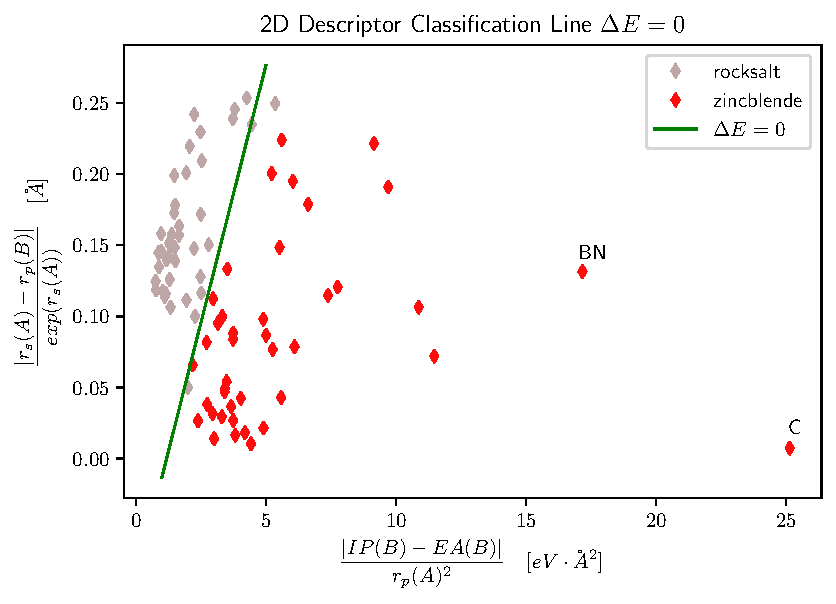
\includegraphics[scale=1]{lasso.pdf}
	\caption{The 2D descriptor classification line which is equivalent to $\Delta E = 0$ in equation (\ref{2D}). Two outliers BN and C (diamond) are labeled}
	\label{line}
\end{figure}
The optimal choice of the amount of $\lambda$ parameters and the amount of contenders $\Theta$ depends on the data set. In this case, there are 53 non-zero coefficients for the lowest value $\lambda_{100}$. Extending the geometric sequence up to $\lambda_{150}$ yields up to 55 non-zero coefficients by the end of the procedure but the recovered models did not change. However, the models did change for choice of 250 values of $\lambda$. The third term of D3 and D4 $$\frac{|r_s(B)-r_p(B)|}{\exp(r_d(A)+r_s(B))}$$ changed to 
$$\frac{|r_s(B)-r_p(B)|}{\exp(r_d(A))}.$$
The change in the errors was barely noticeable. In fact, the biggest change was 1\% increase in MaxAE of the 4D descriptor which suggests the method actually performed slightly worse with a more expensive setting.
The value of $\Theta$ was increased gradually to 35, 40, 45 and finally 50. The models recovered did not change with $\Theta > 30$. Examining the $\Theta$ set shows that there are 15 and 54 pairs of columns with the absolute value of the Pearson correlation coefficient higher than 0.98 and 0.95 respectively. The two very competitive features of the 1D descriptor (labeled 819) and the first term of 2D descriptor (labeled 966) show Pearson correlation coefficient of 0.985. This is the aforementioned problem of correlation between the primary features and consequently, the whole feature space.

\subsection{Cross Validation, Sensitivity Analysis and Extrapolation}
We perform a thorough study of the used methodoly to develop an idea of how reliable the results we managed to obtain really are.

\subsubsection{Leave One Out Cross Validation (LOOCV)}
Simple LOOCV was employed. In total 82 fits of the LASSO+$\ell_{0}$ were performed - each material was the test set once. The results are reported in Table \ref{RMSE_LOOCV}. Average RMSE and MaxAE are the same measure of error for LOOCV so only average RMSE over all test materials is reported - each material was a test datapoint once.
\begin{table}[H]
	\centering
	\begin{tabular}{lllll} 
		\hline
		In eV  & 1D   & 2D  & 3D   & 4D    \\ 
		\hline
		RMSE CV   & 0.132 & 0.104 & 0.085 & 0.062  \\
		\hline
	\end{tabular}
	\caption{The LOOCV RMSE for 1D, 2D, 3D, 4D descriptors}
	\label{RMSE_LOOCV}
\end{table}
\subsubsection{Complexity of the Feature Space} \label{complexity}
The feature space was divided into 6 tiers. We want to see how well the LASSO+$\ell_{0}$ method can navigate the feature space. The division rule is the number of operations needed to build the final feature from the primary features:
% Table 1.4, (1.5) section 1.4.5.2
\begin{itemize}
	\item Tier 0 - the 14 primary features
	\item Tier 1 - 1 operation (unary or binary), e. g. $|IP(A)+IP(B)|$ or $r_s(A)^2$. 164 features in total
	\item Tier 2 - 2 operations, e .g. $\exp\big[r_s(A)^2\big]$ or $ \exp\big[r_d(B) + r_s(A)\big]$. 596 features in total
	\item Tier 3 - 3 operations, e. g. $\exp\big[\big(r_d(B) + r_s(A)\big)^2 \big]$. 1669 features in total
	\item Tier 4 - 4 operations, e. g. $\frac{|r_p(A)-r_s(B)|}{\exp\big[r_p(B)^2\big]}$. 3566 features in total
	\item Tier 5 - 5 operations, e. g. $\frac{|r_s(A)-r_d(B)|}{\exp[(r_s(A)+r_d(B))^2]}$. 4376 features in total
\end{itemize}
Then, 6 feature subspaces are generated and LASSO+$\ell_{0}$ is applied to them. Each feature subspace includes its tier as well as all lower tiers, e. g. Tier 2 feature subspace includes Tier 0, Tier 1 and Tier 2 descriptors. Given the small size of the data set, the cross validation approach of verification of the model was chosen. The data is split at random into two parts consisting of 10\% and 90\% of the data (this means 75 measurements for training and 7 measurements for testing). The model is learned on the train set and the RMSE and MaxAE are evaluated on the test set. The random split is carried out 150 times to gain a good statistic. The average RMSE and MaxAE after the procedure is reported in Table \ref{feature_space_cv}.

\begin{table}[H]
	\centering
	\begin{tabular}{llllllll} 
		\hline
		\multicolumn{2}{l}{In eV } & Tier 0 & Tier 1 & Tier 2 & Tier 3 & Tier 4 & Tier 5  \\ 
		\hline
		\multirow{2}{*}{1D} & RMSE   & 0.262   & 0.187   & 0.162   & 0.159   & 0.172   & 0.172    \\ 
		
		& MaxAE  & 0.529   & 0.380   & 0.304    & 0.305    & 0.340   & 0.340    \\ 
		\hline
		\multirow{2}{*}{2D} & RMSE   & 0.202    & 0.192   & 0.138   & 0.103    & 0.129   & 0.129    \\ 
		
		& MaxAE  & 0.404   & 0.394   & 0.257   & 0.180   & 0.246   & 0.247    \\ 
		\hline
		\multirow{2}{*}{3D} & RMSE   & 0.190   & 0.145   & 0.133   & 0.079   & 0.108   & 0.110    \\ 
		
		& MaxAE  & 0.418   & 0.294   & 0.267   & 0.144   & 0.217   & 0.220    \\ 
		\hline
		\multirow{2}{*}{4D} & RMSE   & 0.194    & 0.136   & 0.102   & 0.086   & 0.112    & 0.093     \\ 
		
		& MaxAE  & 0.415   & 0.266   & 0.194   & 0.167   & 0.233   & 0.187    \\
		\hline
	\end{tabular}
	\caption{L10\%OCV RMSE and MaxAE of cross validation with different feature space sizes}
	\label{feature_space_cv}
\end{table}
We observed expected reduction in test errors when the complexity of the feature subspace increases. However, the minimum was found to be for Tier 3 feature subspace size. This is not in accord with \parencite{ghiringhelli17}. The cause of this has been investigated and the reason is that upon cross validation, it is not guaranteed the best descriptors make it into the $\Theta$ set. If the sought best descriptors are artificially added into $\Theta$, they are chosen every single time. The conclusion is that the richness of the higher tiers which contain many highly correlated features combined with a small dataset leads to unstable behavior when cross validation scheme is employed. One solution to this problem would be increasing the size of the $\Theta$ set. This is not a big problem for 1D and 2D descriptor recovery but can become cumbersome with 3D and 4D descriptors where the $\binom{\Theta}{3}$ and $\binom{\Theta}{4}$ can be too big to be advantageous in terms of time.
\subsubsection{Sensitivity Analysis}
Sensitivity analysis aims to find which features affect the model the most and how much the model depends on certain values of the features. The LASSO+$\ell_{0}$ finds the best descriptor from the feature space generated by the primary features. Applying noise to the primary features and the fitted property is a way of determining the effect of numerical inaccuracies of the DFT calculations and ultimately validates the model and the physical relationship which was found.
\paragraph{Noised Primary Features}
In this series of tests, we multiply one feature with Gaussian noise with mean 1 and standard deviation $\sigma$ taken from $\{0.001, 0.01, 0.03, 0.05, 0.1, 0.13, 0.3\}$ for every test. The feature space is then generated from the primary features where one is always noised.
\begin{table}[H]
	\centering
	\scriptsize
	\begin{tabular}{llrrrrrrr} 
	\hline
	Feature                  & \multicolumn{1}{c}{Quantity} & \multicolumn{7}{c}{ Gaussian noise $\mathcal{N}(1,\sigma)$}                                                                \\ 
	\hline
	&                              & $\sigma = 0.001$ & $\sigma = 0.010$ & $\sigma = 0.030$ & $\sigma = 0.05$ & $\sigma = 0.100$ & $\sigma = 0.130$ & $\sigma = 0.300$  \\ 
	\hline
	\multirow{3}{*}{$IP(A)$}   & Recovery of all data D2 [\%] & 0.74          & 0.65          & 0.31          & 0.18         & 0             & 0             & 0              \\
	& Recovery of LOOCV D2 [\%]    & 0.95          & 0.83          & 0.05          & 0            & 0             & 0             & 0              \\
	& Recovery of L10\%CV D2 [\%]  & 0.92          & 0.5           & 0.36          & 0            & 0             & 0             & 0              \\ 
	\hline
	\multirow{3}{*}{$EA(A)$}   & Recovery of all data D2 [\%] & 0.74          & 0.75          & 0.73          & 0.71         & 0.7           & 0.67          & 0.62           \\
	& Recovery of LOOCV D2 [\%]    & 1             & 0.99          & 0.95          & 0.91         & 0.83          & 0.56          & 0.82           \\
	& Recovery of L10\%CV D2 [\%]  & 1             & 0.98          & 0.92          & 0.9          & 0.8           & 0.84          & 0.52           \\ 
	\hline
	\multirow{3}{*}{$IP(B)$}   & Recovery of all data D2 [\%] & 0.74          & 0.73          & 0.36          & 0.25         & 0.02          & 0.02          & 0              \\
	& Recovery of LOOCV D2 [\%]    & 0.98          & 0.7           & 0.24          & 0.33         & 0.11          & 0.02          & 0.02           \\
	& Recovery of L10\%CV D2 [\%]  & 1             & 0.86          & 0.82          & 0.36         & 0.24          & 0.22          & 0.22           \\ 
	\hline
	\multirow{3}{*}{$EA(B)$}   & Recovery of all data D2 [\%] & 0.75          & 0.71          & 0.6           & 0.45         & 0.39          & 0.42          & 0.14           \\
	& Recovery of LOOCV D2 [\%]    & 0.99          & 0.98          & 0.49          & 0.28         & 0.24          & 0.26          & 0.24           \\
	& Recovery of L10\%CV D2 [\%]  & 1             & 0.86          & 0.88          & 0.7          & 0.82          & 0.5           & 0.46           \\ 
	\hline
	\multirow{3}{*}{$H(A)$}    & Recovery of all data D2 [\%] & 0.74          & 0.74          & 0.74          & 0.73         & 0.75          & 0.74          & 0.87           \\
	& Recovery of LOOCV D2 [\%]    & 1             & 0.98          & 0.85          & 0.84         & 0.83          & 0.83          & 0.83           \\
	& Recovery of L10\%CV D2 [\%]  & 0.98          & 1             & 0.76          & 0.8          & 0.76          & 0.72          & 0.6            \\ 
	\hline
	\multirow{3}{*}{$L(A)$}    & Recovery of all data D2 [\%] & 0.74          & 0.75          & 0.75          & 0.75         & 0.75          & 0.75          & 0.71           \\
	& Recovery of LOOCV D2 [\%]    & 1             & 1             & 1             & 1            & 0.99          & 1             & 1              \\
	& Recovery of L10\%CV D2 [\%]  & 1             & 1             & 0.96          & 0.92         & 0.96          & 0.96          & 0.92           \\ 
	\hline
	\multirow{3}{*}{$H(B)$}    & Recovery of all data D2 [\%] & 0.74          & 0.74          & 0.74          & 0.73         & 0.72          & 0.74          & 0.71           \\
	& Recovery of LOOCV D2 [\%]    & 1             & 1             & 1             & 1            & 0.85          & 0.98          & 1              \\
	& Recovery of L10\%CV D2 [\%]  & 1             & 0.98          & 0.98          & 0.78         & 0.92          & 0.92          & 0.92           \\ 
	\hline
	\multirow{3}{*}{$L(B)$}    & Recovery of all data D2 [\%] & 0.74          & 0.74          & 0.77          & 0.71         & 0.69          & 0.66          & 0.75           \\
	& Recovery of LOOCV D2 [\%]    & 1             & 0.99          & 0.99          & 0.98         & 0.99          & 0.98          & 0.83           \\
	& Recovery of L10\%CV D2 [\%]  & 1             & 0.96          & 0.98          & 0.96         & 0.94          & 0.92          & 0.8            \\ 
	\hline
	\multirow{3}{*}{$r_s(A)$} & Recovery of all data D2 [\%] & 0.74          & 0.74          & 0.72          & 0.71         & 0.65          & 0.51          & 0              \\
	& Recovery of LOOCV D2 [\%]    & 0.99          & 0.99          & 0.99          & 0.85         & 0.87          & 0.01          & 0.02           \\
	& Recovery of L10\%CV D2 [\%]  & 0.98          & 0.92          & 0.82          & 0.82         & 0.42          & 0.68          & 0.1            \\ 
	\hline
	\multirow{3}{*}{$r_p(A)$} & Recovery of all data D2 [\%] & 0.74          & 0.67          & 0.49          & 0.31         & 0             & 0             & 0              \\
	& Recovery of LOOCV D2 [\%]    & 0.99          & 0.93          & 0.02          & 0.12         & 0             & 0             & 0              \\
	& Recovery of L10\%CV D2 [\%]  & 0.96          & 0.8           & 0.36          & 0            & 0             & 0             & 0              \\ 
	\hline
	\multirow{3}{*}{$r_d(A)$} & Recovery of all data D2 [\%] & 0.74          & 0.74          & 0.74          & 0.74         & 0.74          & 0.74          & 0.74           \\
	& Recovery of LOOCV D2 [\%]    & 1             & 1             & 1             & 0.99         & 0.98          & 0.99          & 0.98           \\
	& Recovery of L10\%CV D2 [\%]  & 1             & 1             & 0.94          & 0.94         & 0.84          & 0.9           & 0.82           \\ 
	\hline
	\multirow{3}{*}{$r_s(B)$} & Recovery of all data D2 [\%] & 0.74          & 0.75          & 0.77          & 0.75         & 0.76          & 0.75          & 0.75           \\
	& Recovery of LOOCV D2 [\%]    & 1             & 1             & 0.95          & 0.98         & 0.94          & 0.9           & 0.95           \\
	& Recovery of L10\%CV D2 [\%]  & 0.96          & 0.88          & 0.88          & 0.78         & 0.8           & 0.78          & 0.78           \\ 
	\hline
	\multirow{3}{*}{$r_p(B)$} & Recovery of all data D2 [\%] & 0.74          & 0.75          & 0.76          & 0.76         & 0.69          & 0.59          & 0              \\
	& Recovery of LOOCV D2 [\%]    & 1             & 0.99          & 0.99          & 0.96         & 0.98          & 0.87          & 0.01           \\
	& Recovery of L10\%CV D2 [\%]  & 0.98          & 0.96          & 0.74          & 0.78         & 0.58          & 0.4           & 0.02           \\ 
	\hline
	\multirow{3}{*}{$r_d(B)$} & Recovery of all data D2 [\%] & 0.74          & 0.75          & 0.67          & 0.67         & 0.71          & 0.67          & 0.72           \\
	& Recovery of LOOCV D2 [\%]    & 0.99          & 0.96          & 0.88          & 0.93         & 0.82          & 0.87          & 0.85           \\
	& Recovery of L10\%CV D2 [\%]  & 0.98          & 0.94          & 0.82          & 0.8          & 0.46          & 0.64          & 0.64           \\
	%\cline{1-9}
	\hline
\end{tabular}
	\caption{Noise applied to the primary features}
	\label{big}
\end{table}
Table \ref{big} summarizes the tests carried out. For every feature and for each noise level $\sigma$, 50 instances of the Gaussian noise are applied to the feature for 50 L10\%OCV procedures and 82 LOOCV procedures which results in a statistic of 2500 samples and 4100 respectively. Noising primary features $EA(A)$, $H(A)$, $L(A)$, $H(B)$, $L(B)$, $r_d(A)$, $r_s(B)$ and $r_d(B)$ has much less effect that the other 6 features where 5 of these appear in the 2D descriptor and the 6th is $IP(A)$ which appears in the expression of the 1D descriptor which is highly correlated with the first expression of the 2D descriptor as mentioned before. Therefore it is not surprising this feature also affects the recovery of the descriptor because it apparently appears to be a part of the best 2D descriptor recovered during cross validation. 
The LOOCV RMSE remained stable throughout tests with its value being 0.1-0.13 eV for all noise levels and noised features except $IP(A)$ where the RMSE rose gradually up to 0.24 eV. The L10\%OCV RMSE remained stable throughout the tests as well at 0.12-0.14 eV and $IP(A)$ was unstable with gradual increase of RMSE up to 0.35 eV.
The percentage of recovery of the 2D descriptor obtained on all data remains stable for the 8 aforementioned features and recovery of the same LOOCV and L10\%OCV descriptors with or without noise is also very stable.
\paragraph{Adding Noise to $\Delta E$}
In this test, the energy difference $\Delta E$ was perturbed with additive noise drafted from uniform distribution $\mathcal{U}(-\delta, \delta)$ where $\delta \in \{0.01, 0.03, 0.1, 0.2\}$. The sources \parencite{ghiringhelli15} and \parencite{ghiringhelli17} do not mention how the relevant subsets of the whole feature space were selected. Therefore, we choose Tier 3 and Tier 4 subspaces of the feature space defined in \ref{complexity}. Their respective sizes 1669 and 3566 match reasonably the original mysterious subsets with sizes 1568 and 2924 respectively. To match the carried out test as much as possible with the limited information, the found 1D, 2D, 3D, 4D descriptors were added into both sets if they were not already present. This is the case for the last term of 3D which is also the third term of 4D and it is also the case for the last term of 4D because it was made using 4 and 5 operations respectively and they do not appear naturally in the feature spaces we selected for this test (see equations (\ref{3D}) and (\ref{4D})). Effectively, the feature space sizes are 1671 and 3567 respectively after the addition. The test was carried out for the 2D descriptor only as in \parencite{ghiringhelli17}. In total, for every noise level in $\delta$, 10 drafts of the random number from the uniform distribution were performed and for each draft, 90\% - 10\% cross validation split was caried out 50 times. This sums to a statistic of 500 prediction samples for each noise level. The results are reported in Table \ref{sense_E}.
\begin{table}[H]
	\centering
	\refstepcounter{table}
	\label{sense_E}
	\begin{tabular}{lllllll} 
		\hline
		Number of features    & \multicolumn{1}{c}{Quantity} & \multicolumn{5}{c}{$\mathcal{U}(-\delta, \delta)$}          \\ 
		\hline
		& \multicolumn{1}{c}{}         & $\delta=0$     & $\delta=0.01$  & $\delta=0.03$  & $\delta=0.1$   & $\delta=0.2$    \\ 
		\hline
		\multirow{4}{*}{1671} & RMSE CV [eV]                  & 0.102 & 0.103 & 0.106 & 0.128 & 0.178  \\ 		
		& AveMaxAE CV [eV]              & 0.180 & 0.180 & 0.187 & 0.228 & 0.319  \\ 		
		& Recovery of all data D2 [\%]  & 94    & 92    & 89.2  & 64    & 15     \\ 		
		& Recovery of L10\%OCV D2 [\%]  & 100   & 96    & 90.4  & 62.8  & 15     \\ 
		\hline
		\multirow{4}{*}{3567} & RMSE CV [eV]                  & 0.130 & 0.129 & 0.131 & 0.148 & 0.185  \\ 
		
		& AveMaxAE CV [eV]              & 0.253 & 0.248 & 0.247 & 0.277 & 0.336  \\ 
		
		& Recovery of all data D2 [\%]  & 42    & 38.8  & 34    & 11.2  & 1      \\ 
		
		& Recovery of L10\%OCV D2 [\%]  & 100   & 88    & 68.8  & 30.2  & 7.4    \\
		\hline
	\end{tabular}
	\caption{RMSE, average MaxAE, recovery rate of 2D descriptor of equation (\ref{2D}) and recovery rate of leave 10\% out cross validation descriptor ($\delta=0$) for the two feature sets with different noise levels}
\end{table}
The drop in performance of the model described by the four quantities is in accord with \parencite{ghiringhelli17}. Understandably, the values differ because our feature spaces are different. The stability of descriptor recovery is measured by two quantities. Recovery of all data D2 means the percentage of times when the 2D descriptor of equation (\ref{2D}) was found upon cross validation and Recovery of L10\%OCV D2 reports the percentage of times when the 2D descriptor of noised data was the same as the 2D descriptor of non-noised data with the same cross validation split. For the smaller feature space, the errors are in great accord with a feature space of similar size \parencite{ghiringhelli17} where the AveMaxAE CV is in exact accord and RMSE CV differs by less than 0.01 eV on all occasion. We found the same behavior of descriptor stability for noise levels up to $\delta=0.03$. The descriptor found by the cross validation procedure almost always matches the one in equation (\ref{2D}) for all noise levels. For the larger feature space, which is much bigger than the one in \parencite{ghiringhelli17}, we can observe trend of worse descriptor recovery success. The RMSE CV and AveMaxAE CV differs by less than 0.02 eV and 0.06 eV respectively on all ocassions even for much bigger feature space. Combined with the low recovery rates, this hints towards the fact, that many competitive models can be recovered from the pool of 30 candidates.
\subsection{Extrapolation Capabilities of the Model}
Two distinct tests were performed to evaluate how the model will hold when a certain group of materials is removed altogether from the training and reserved as a test set.
\paragraph{BN and C (diamond)}
In this test, two most stable zincblende materials (labeled in Figure \ref{line}) are chosen as the test set and the model is trained on the remaining 80 datapoints. It is worthwhile to note that the recovered models can be different from the ones we receive after training on the whole dataset. This effect might be amplified by the extraordinary stability of these materials. The predictions and the actual LDA energies are listed in Table \ref{C_BN}.
\begin{table}[H]
	\centering
	\begin{tabular}{llllll} 
		\hline
		In eV & 1D    & 2D    & 3D    & 4D    & LDA    \\ 
		\hline
		C     & 1.188 & 1.638 & 1.637 & 2.937 & 2.638  \\ 		
		BN    & 0.826 & 1.096 & 1.387 & 1.754 & 1.713  \\
		\hline
	\end{tabular}
	\caption{Model performances for C and BN as the test set}
	\label{C_BN}
\end{table}
In \parencite{ghiringhelli17}, only 2D descriptor model was tested. We list all the models because it illustrates the prediction improvement with increased model complexity. Particularly, the 4D descriptor performs much better than any other. The difference between our prediction with 2D descriptor and \parencite{ghiringhelli17} differs by 0.2 eV for diamond and less than 0.3 eV for BN. All descriptors always classify diamond and BN as zincblende structures.
Out of curiousity, to demonstrate leakage of information from the test set into the training procedure, we forced the 2D descriptor to be the one in equation (\ref{2D}). That is, we remove all but 2 contenders from $\Theta$ - we put $$\Theta = \Big\{ \frac{|IP(B)-EA(B)|}{r_p(A)^2}, \frac{|r_s(A)-r_p(B)|}{\exp(r_s(A))} \Big\}$$ and consequently, the model is trained on 80 datapoints and prediction for diamond and BN is made. The results of absolute error of 0.032 eV for diamond and 0.130 eV for BN is surprisingly low even though they are obviously spurious.
\paragraph{Carbon Out}
In this test, all compounds containing carbon were removed from the training. Namely, it is C (diamond), SiC, GeC, SnC. The model was trained on the remaining 78 datapoints. Again, 4 models are listed in Table \ref{carbon} whereas \parencite{ghiringhelli17} lists only performance of the 2D descriptor model.
\begin{table}[H]
	\centering
	\begin{tabular}{llllll} 
		\hline
		In eV & 1D    & 2D    & 3D    & 4D    & LDA    \\ 
		\hline
		C     & 1.438 & 1.339 & 1.561 & 2.315 & 2.638  \\ 		
		SiC   & 0.485 & 0.469 & 0.527 & 0.590 & 0.668  \\ 
		GeC   & 0.443 & 0.461 & 0.502 & 0.597 & 0.808  \\ 
		SnC   & 0.215 & 0.228 & 0.244 & 0.259 & 0.450  \\
		\hline
	\end{tabular}
	\caption{Model performances for C, SiC, GeC, SnC as the test set}
	\label{carbon}
\end{table}
The 2D descriptor performance exactly matches the results in \parencite{ghiringhelli17} for 3 compounds containing carbon. For diamond, our error is lower by 0.03 eV. Our 4D descriptor model performs excellently for diamond given the fact it has never seen carbon.

%\subsubsection{Conclusion}
%The experiment presented in \parencite{ghiringhelli15} and \parencite{ghiringhelli17} was carried out. The feature space defined and generation matched almost exactly the feature space in the publications. The corresponding 1D, 2D, 3D descriptors were recovered successfully and we also presented the 4D descriptor. The LASSO+$\ell_{0}$ was analyzed and its properties examined. The performance of the found models was tested under LOOCV, L10\%OCV combined with tier-based feature space analysis of the performance of the LASSO+$\ell_{0}$ method and thorough sensitivity analysis with focus on the sensitivity of the primary features and then sensitivity of the energy. Lastly, the extrapolation capabilities of the 1D, 2D, 3D and 4D models were examined for two most stable structures BN and diamond and then for compounds which contaion carbon. These test were successful for all recovered descriptors where the most complex 4D descriptor performed the best.
\chapter{Transparent Conducting Oxides Experiment}
Transparent conducting oxides are a class of materials which are widely used in optical electronics, solar cells, LEDs, touch screens, lasers and more. The compound needs to be both electrically conductive and transparent to visible light to be usable for such applications. Alloys of group-III oxides have been experimentally examined to be worthwhile contenders for these use cases. Namely, it is $Al_2 O_3$, $Ga_2 O_3$ and $In_2 O_3$. We shall denote an alloy with $x$\% $Al_2 O_3$, $y$\% $Ga_2 O_3$ and $z$\% $In_2 O_3$ as $(Al_{x}Ga_{y}In_{z})_2 O_3$ and $x+y+z=1$. The problem is that the aforementioned three oxides exhibit different properties and it is unclear whether an alloy with the given composition will be stable or possess desired conductivity. The goal of this experiment is to find a regression model which accurately predicts the stability and transparency of group-III oxide alloys \parencite{sutton18}, \parencite{sutton19}.
%A dataset of 2991 transparent conductors from the Nomad2018 Predicting Transparent Conductors Kaggle competition is available \parencite{sutton18}.

\section{The Dataset}
In this section, the structure of the used dataset will be explained and some of its properties examined. The dataset available consists of the Nomad2018 Predicting Transparent Conductors Kaggle competition dataset (3000 datapoints) that was cleaned which results in 2991 distinct materials (the 9 datapoints turned out be duplicates). Additionally, the raw text files of the DFT calculation were provided by Fritz Haber Institute of the Max Planck Society in Berlin. These files contain additional data which consists of non-converged materials. In other words, we include some of the data generated during the calculation and add them into the dataset. Unfortunately, the files contain only a few last relaxation step (see Section \ref{DFT} for an explanation of the calculation methodology). The dataset of the starting configuration (called Vegard dataset \parencite{NOMAD_repo}) with corresponding DFT calculation results was downloaded from the NOMAD Repository \parencite{NOMAD_repo}.

\tikzstyle{block} = [rectangle, draw, fill=white, text width=6em, text centered, minimum height=5em]

\begin{figure}[h]
	\begin{tikzpicture}[thick,scale=0.6, every node/.style={scale=0.75}, node distance = 4cm, auto]
		\node [block] (vegard) {Vegard data};
		
		\node [block, right of=vegard] (rsn) {1st relaxation step data};
		
		\node [block, right of=rsn] (dots) {...};
		
		\node [block, right of=dots] (nth) {$n$th relaxation step data};
		
		\node [block, right of=nth] (dots2) {...};
		
		\node [block, right of=dots2] (final) {Last relaxation step data};
		
		\scriptsize
		\draw [->] (vegard) -- node {calculation} (rsn);
		
		\draw [->] (rsn) -- node {calculation} (dots);
		
		\draw [->] (dots) -- node {calculation} (nth);
		
		\draw [->] (nth) -- node {calculation} (dots2);
		
		\draw [->] (dots2) -- node {calculation} (final);
	\end{tikzpicture}
	\caption{The flowchart explaining the connections of the three datasets for every material}
\end{figure}
The last relaxation step is the final configuration of the material. The number of relaxation steps is not a priori known therefore every material has different amount of relaxation steps. The reason behind this is the iterative nature of the relaxation procedure. In total, this way we managed to gather additional 2991 Vegard datapoints and additional 34219 relaxation datapoints to the 2991 datapoints from the Kaggle competition. The datasets can be found in a github repository \parencite{github}. To gain intuition of the behavior of the DFT calculation, an example is presented in Figure \ref{relaxation} and a barplot of the amount of relaxation steps for every material is in Figure \ref{rsn_barplot}.

\begin{figure}[H]       
	%\fbox{}   
	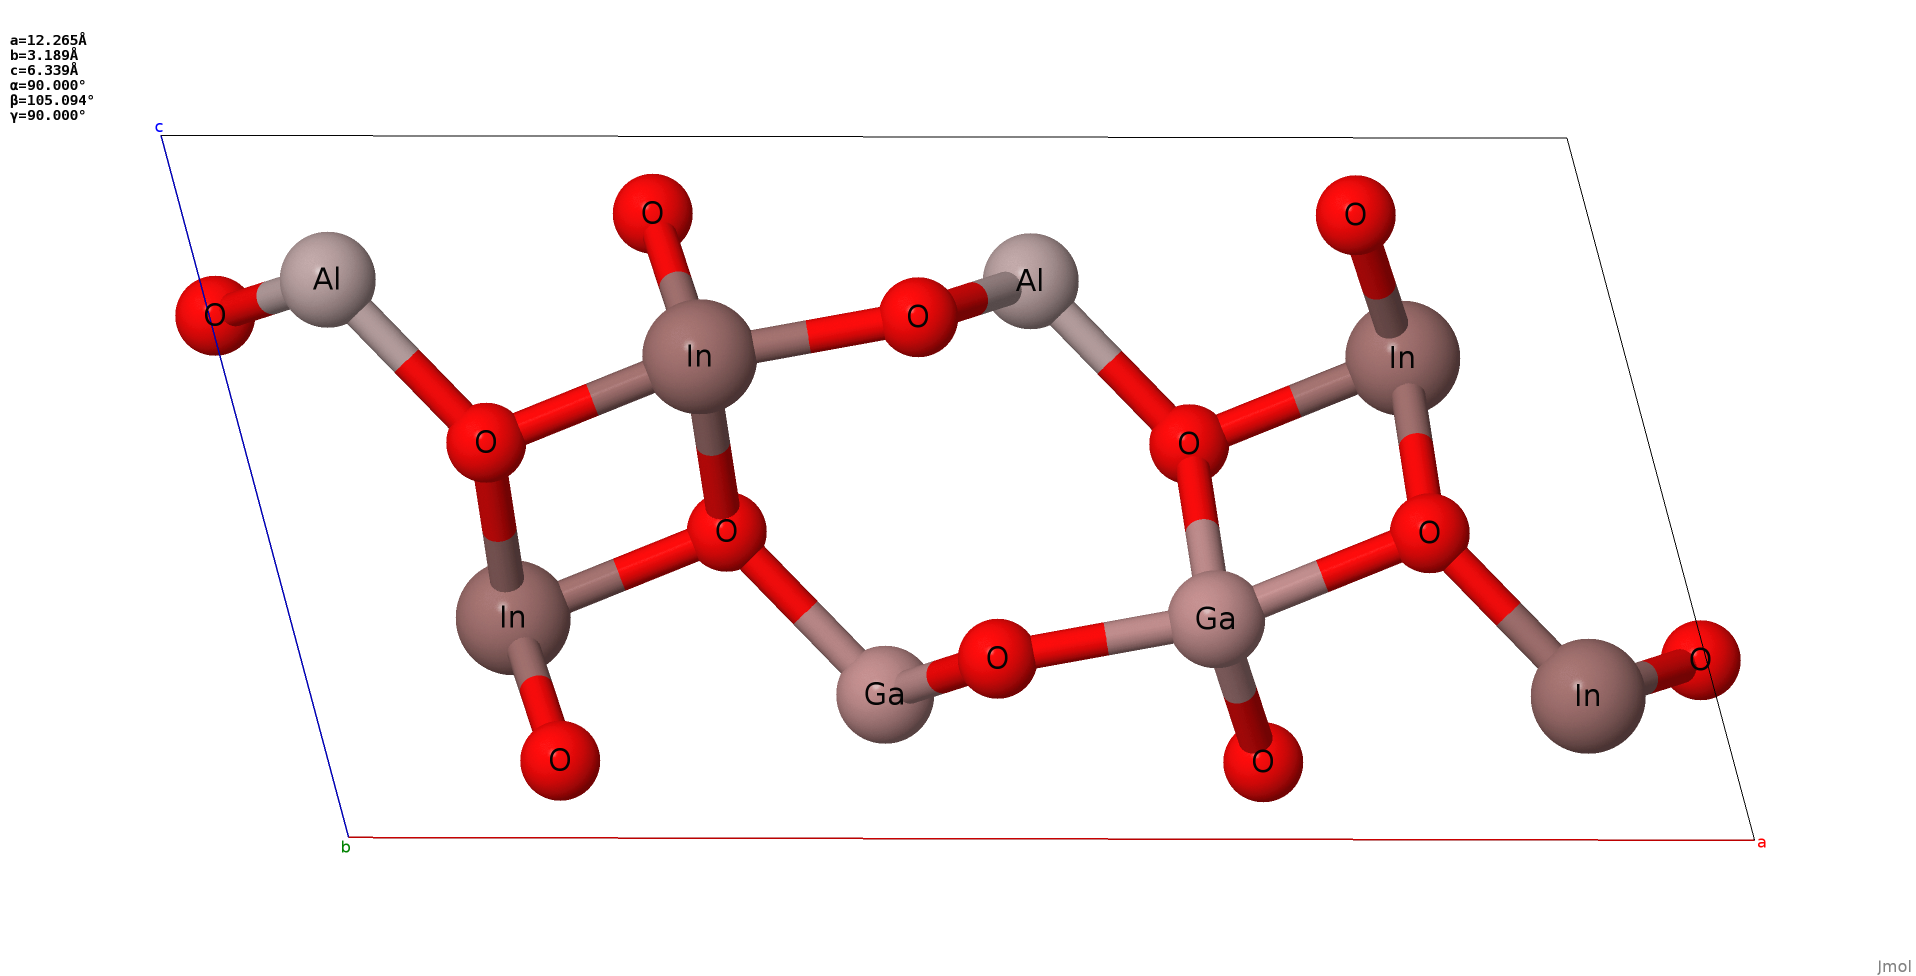
\includegraphics[scale=0.25]{train_id_20_vegard_hotovo.png}
	%\hspace{30px}
	%\fbox{}
	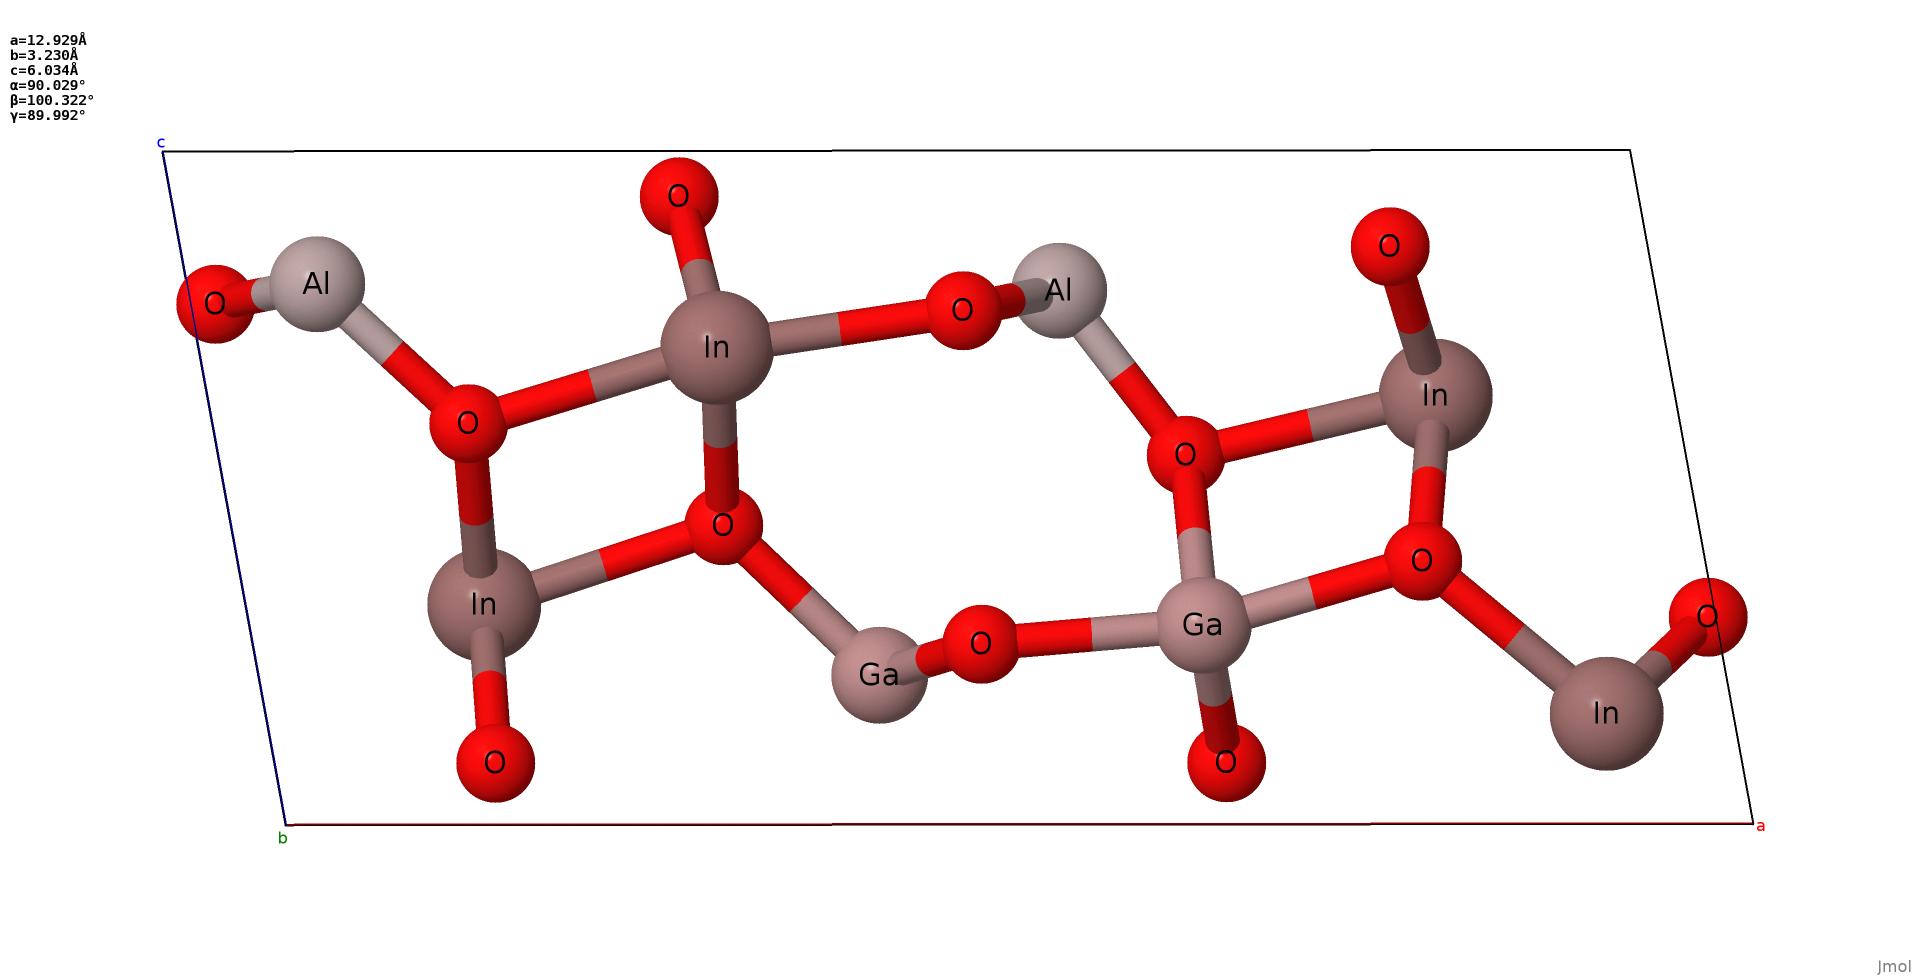
\includegraphics[scale=0.25]{train_id_20_final_hotovo.png}
	%\hspace{30px}
	%\fbox{}
	\caption{Alloy $(Al_{0.25}Ga_{0.25}In_{0.5})_2 O_3$ relaxation example. Top: Vegard data positions. Bottom: The last relaxation data position (final data). This material has only one relaxation step - after only one iteration, the procedure converged. Notice the change in the lattice vectors as well as the change in atomic position of the oxygen and indium on the right \parencite{jmol}}
	\label{relaxation}
\end{figure}

\begin{figure}[H]
	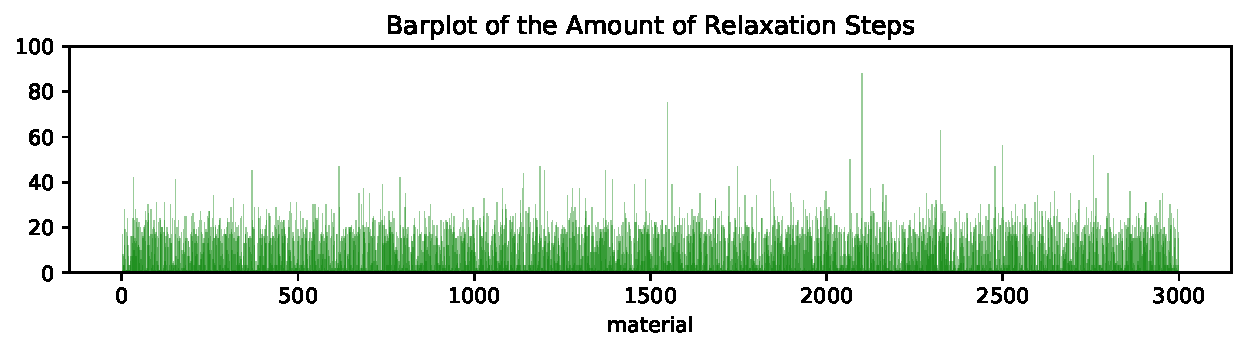
\includegraphics[scale=0.8]{rsn.pdf}
	\caption{The amount of relaxation steps recovered from the files for 2991 materials. The mean value of relaxation steps is 12.440}
	\label{rsn_barplot}
\end{figure}

A very important detail of the Kaggle competition is that the atomic positions provided are from the Vegard dataset - the initial positions before relaxation. However, the provided quantities to be predicted (formation energy, bandgap energy) correspond to the final dataset. This is practical: a model which would need the final positions does not save any time because the calculation of the final configuration is the procedure we would like mimic with our model because of its computational difficulty. However, this was not explicitly stated during the competition. Also, the ability to analyze the relaxation procedure and compare the initial data with the final data can bring valuable insight which was not possible.

For coherence, our datasets were constructed to possess much more natural structure and the atomic positions correspond to the calculated energies of the given relaxation step. If need be, the atomic positions and calculated energies can be matched as seems fit for the given task (e.g. combine Vegard positions and final energies etc.).

%The Vegard dataset was not mixed into the rest of the data because of its nature. It does not hold the information about the DFT procedure.

\subsection{Formation Energy and Bandgap}
The two physically meaningful quantities we want to predict are formation energy and band gap of the alloy. The formation energy is defined as the difference between the calculated DFT energy of the alloy $(Al_{x}Ga_{y}In_{z})_2 O_3$ and the calculated DFT energy of the pure oxides $\alpha$-$Al_2 O_3$, $\beta$-$Ga_2 O_3$ and $c$-$In_2 O_3$

\begin{equation}
	E_f = E[(Al_{x}Ga_{y}In_{z})_2 O_3] - xE[Al_2 O_3] - yE[Ga_2 O_3] - zE[In_2 O_3] 
	\label{formation}
\end{equation}
where $x = \frac{N_{Al}}{N_{Al}+N_{Ga}+N_{In}}$, $y = \frac{N_{Ga}}{N_{Al}+N_{Ga}+N_{In}}$ and $z = \frac{N_{In}}{N_{Al}+N_{Ga}+N_{In}}$ as defined in \parencite{sutton19}. The $\alpha$, $\beta$ and $c$ in the name of the oxides determine the space group of the crystal for the given oxide (one oxide can crystallize in multiple space groups). The traditional definition of the formation energy is the energy of the compound minus the individual atomic energies. Therefore the difference is that the reference is the pure oxides and not individual atoms. The physical meaning of the formation energy is that the bigger the value, the higher is the stability of the alloy in terms of degradation and loss of desirable properties. It is also possible that this quantity has negative value for the given material. This means the alloy is not a stable crystal and should degrade.

The band structure of a solid material is the manifestation of the principles of the quantum mechanical behavior of electrons in crystals. The shape of the band structure determines the response of the material to light (transparency to certain wavelengths, absorption of certain wavelengths etc.), changes in temperature and classifies to materials to metals, semiconductors and insulators. The bandgap is the shortest distance between the conduction and valence bands of the band structure and it is the energy needed to excite the electron from the top valence band to the bottom of the conduction band \parencite{sutton19}, \parencite{kraus16}. We desire to predict this value to be able to determine if the material at hand would be useful for the given application.

\section{Results and Discussion of ngram}
The motivation and general discussion of ngram was presented in Chapter \ref{feature_engineering}. We implement the ngram descriptor and analyze some unclear heuristic choices which were made during its definition and construction. Then, the proposed extension is implemented and tested on the competition dataset and the mined dataset which extends the competition dataset.
\subsection{Analysis}
The ngram representation proved to be the best in the Nomad2018 Predicting Transparent Conductors Kaggle competition because of its ability to utilize the structural information (atomic positions and lattice vectors) in an approximative way. The robustness of the condition in equation (\ref{decision}) was tested for the relaxation data in the following way: the coordination environment of all atoms of the first relaxation step is compared with the coordination environment of all atoms in the second relaxation step. The third relaxation step is compared with the second and so on until we reach the last relaxation step (final data).

This procedure was carried out for the combination of Shannon ionic radii used in the competition (coordination VI ionic radii for metals and coordination II ionic radius for oxygen, see Table \ref{shannon_radii}). The condition in (\ref{decision}) holds for remarkable 2635 materials out of 2991. The robustness of the coordination environment of the Vegard data and the final configuration was tested as well and all 2991 materials undergo a change in the coordination environments between the starting Vegard configuration and finishing final configuration. An example of the difference can be seen on the unigrams in Figure \ref{unigram_vegard_final}.
\begin{figure}[H]
	\centering
	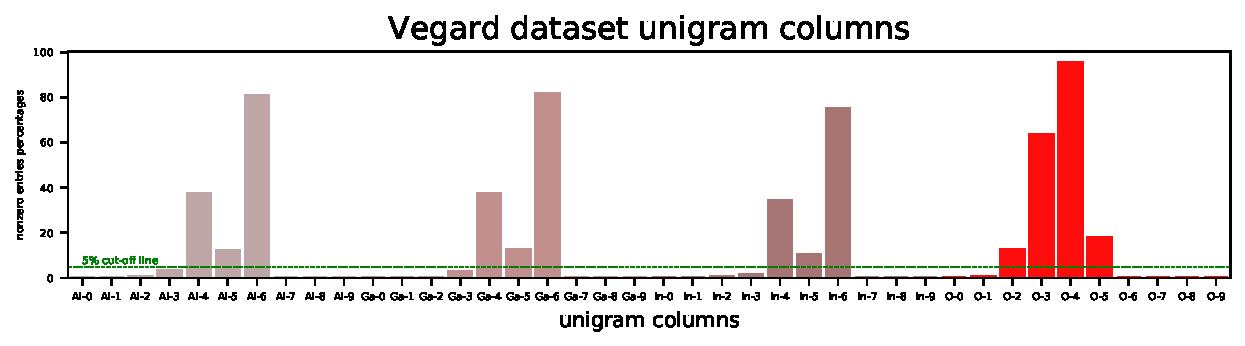
\includegraphics[scale=0.8]{vegard_nonzero_unigram_competition.pdf}
	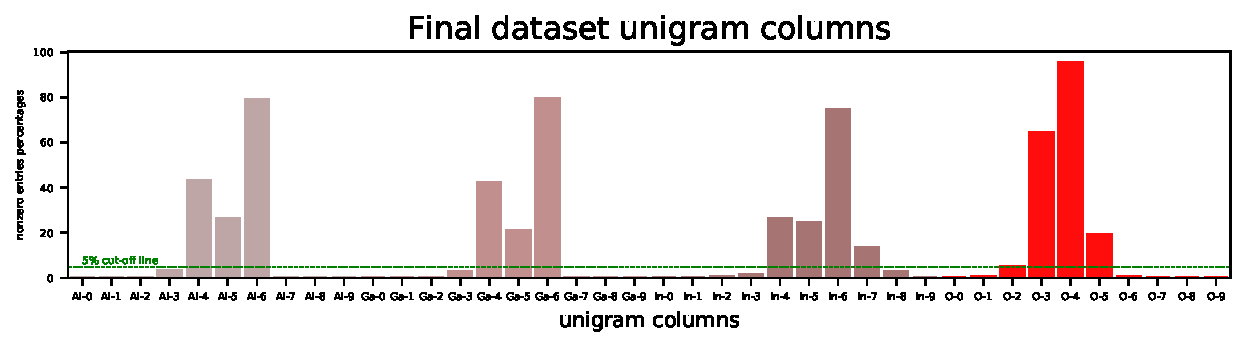
\includegraphics[scale=0.8]{final_nonzero_unigram_competition.pdf}
	\caption{The difference between nonzero entries of the unigram for vegard dataset and final dataset. There is a substantial increase of nonzero columns after the whole DFT calculation. Notice the changes for indium. The 5\% cutoff line is in green.}
	\label{unigram_vegard_final}
\end{figure}
Consequently, it was tested whether the unigram columns which are zero for more than 95\% of the materials carry any substantial information. This was tested for the Vegard and the final dataset. The reduction is from 21 nonempty columns of Vegard dataset to 13 columns (the same 13 columns as in \parencite{sutton19}) and 26 to 14 columns for the final dataset. The reduced matrices were used for training KRR models which predict the formation and bandgap energies. The reduction of the columns of the matrices resulted in significant loss of prediction accuracy of the models and we advice against such practices and such reduction will not be discussed further.

The choice of the value Shannon ionic radii is debatable. We get to choose these 4 values from many but the best values are not a priori known. The possibility to perform an exhaustive search over all possible combinations of values from the Table \ref{shannon_radii} would be computationally extremely expensive for the relaxation dataset (considering the cross validation procedures for both the formation energy as well as bandgap of the KRR models). A worthwhile compromise was tested and the mean value of the Shannon radii for every atom species was taken as the chosen value. This is outlined in equation (\ref{shannon_calc}).
\begin{equation}
	\begin{aligned}
		R^S_{Al} &= \frac{0.39+0.48+0.535}{3} = 0.468 \, \AA\\
		R^S_{Ga} &= \frac{0.47+0.55+0.62}{3} = 0.547 \, \AA\\
		R^S_{In} &= \frac{0.62+0.8+0.92}{3} = 0.780 \, \AA\\
		R^S_O &= \frac{1.35+1.36+1.38+1.4+1.42}{5} = 1.382 \, \AA
	\end{aligned}
\label{shannon_calc}
\end{equation}
The geometric mean was also considered but the values of geometric mean vary from the arithmetic mean negligibly so we chose not test these values. The choice of the correct shape of the inequality in equation (\ref{decision}) is up to debate as well since it includes multiple assumptions which have a physical background but are still heuristic in their nature.

The robustness test of relaxation steps was performed for the Shannon ionic radii averages from (\ref{shannon_calc}). The condition in (\ref{decision}) holds for 1612 materials out of 2991. The robustness of the coordination environment of the Vegard data and the final configuration was tested again and all 2991 materials undergo a change in the coordination environments. The Shannon ionic radii averages performed slightly worse for unigrams and bigrams. The adjustment was not an improvement and we will not discuss it further.

The combination of Shannon ionic radii VI for Al and Ga, coordination VIII for In and coordination VI for O was tested next. We chose the maximum of ionic radii for metals and coordination VI for oxygen because it is the most likely coordination for oxygen. It is possible that the change of the value of the Shannon ionic radius for oxygen does not bring anything new because the values are very similar for all coordinations. The value of Shannon radius for coordination VIII of In is very large and introduces coordinations of indium up to 11 in the datasets. This is not physically justifiable and one can even view it as spurious. This combination of radii resulted in great increase of test error and it is clear that the main culprit is the creation of spurious coordination as the result of choosing the maximal values of Shannon radii for metals.

The minimal values for radii were tested and performed slightly worse. The maximum values for all atoms performed in a similar fashion. 

It appears the choice II for O and VI for Al, Ga and In holds the best physical meaning and we will use them in our conducted experiments and the choice of Shannon radii will not be discussed further.

%The relaxation dataset of 34219 datapoints unfortunately does not bring any improvement of the models. Every single experiment carried out resulted in the same or slightly worse prediction error. Also, it is incredibly computationally demanding to create KRR models with such a huge dataset.

\subsection{Modelling}

%\chapter{Materials Project Experiment}
%something
\chapter*{Conclusion}
\pagestyle{plain}

\addcontentsline{toc}{chapter}{Conclusion}

something

\appendix
\chapter{The Rocksalt-Zincblende Classification Dataset}
% the \\ insures the section title is centered below the phrase: AppendixA
\begin{table}[H]
	\begin{tabular}{rlrrrrrrrr}
		\hline
		Z & Name   &      IP &     EA &     EN &    HOMO &   LUMO &   $r_s$ &   $r_p$ &   $r_d$ \\
		\hline
		3 & Li     &  -5.329 & -0.698 &  3.014 &  -2.874 & -0.978 & 1.652 & 1.995 & 6.93  \\
		4 & Be     &  -9.459 &  0.631 &  4.414 &  -5.6   & -2.098 & 1.078 & 1.211 & 2.877 \\
		5 & B      &  -8.19  & -0.107 &  4.149 &  -3.715 &  2.248 & 0.805 & 0.826 & 1.946 \\
		6 & C      & -10.852 & -0.872 &  5.862 &  -5.416 &  1.992 & 0.644 & 0.63  & 1.631 \\
		7 & N      & -13.585 & -1.867 &  7.726 &  -7.239 &  3.057 & 0.539 & 0.511 & 1.54  \\
		8 & O      & -16.433 & -3.006 &  9.72  &  -9.197 &  2.541 & 0.462 & 0.427 & 2.219 \\
		9 & F      & -19.404 & -4.273 & 11.839 & -11.294 &  1.251 & 0.406 & 0.371 & 1.428 \\
		11 & Na     &  -5.223 & -0.716 &  2.969 &  -2.819 & -0.718 & 1.715 & 2.597 & 6.566 \\
		12 & Mg     &  -8.037 &  0.693 &  3.672 &  -4.782 & -1.358 & 1.33  & 1.897 & 3.171 \\
		13 & Al     &  -5.78  & -0.313 &  3.046 &  -2.784 &  0.695 & 1.092 & 1.393 & 1.939 \\
		14 & Si     &  -7.758 & -0.993 &  4.375 &  -4.163 &  0.44  & 0.938 & 1.134 & 1.89  \\
		15 & P      &  -9.751 & -1.92  &  5.835 &  -5.596 &  0.183 & 0.826 & 0.966 & 1.771 \\
		16 & S      & -11.795 & -2.845 &  7.32  &  -7.106 &  0.642 & 0.742 & 0.847 & 2.366 \\
		17 & Cl     & -13.902 & -3.971 &  8.936 &  -8.7   &  0.574 & 0.679 & 0.756 & 1.666 \\
		19 & K      &  -4.433 & -0.621 &  2.527 &  -2.426 & -0.697 & 2.128 & 2.443 & 1.785 \\
		20 & Ca     &  -6.428 &  0.304 &  3.062 &  -3.864 & -2.133 & 1.757 & 2.324 & 0.679 \\
		29 & Cu     &  -8.389 & -1.638 &  5.014 &  -4.856 & -0.641 & 1.197 & 1.68  & 2.576 \\
		30 & Zn     & -10.136 &  1.081 &  4.527 &  -6.217 & -1.194 & 1.099 & 1.547 & 2.254 \\
		31 & Ga     &  -5.818 & -0.108 &  2.963 &  -2.732 &  0.13  & 0.994 & 1.33  & 2.163 \\
		32 & Ge     &  -7.567 & -0.949 &  4.258 &  -4.046 &  2.175 & 0.917 & 1.162 & 2.373 \\
		33 & As     &  -9.262 & -1.839 &  5.551 &  -5.341 &  0.064 & 0.847 & 1.043 & 2.023 \\
		34 & Se     & -10.946 & -2.751 &  6.848 &  -6.654 &  1.316 & 0.798 & 0.952 & 2.177 \\
		35 & Br     & -12.65  & -3.739 &  8.194 &  -8.001 &  0.708 & 0.749 & 0.882 & 1.869 \\
		37 & Rb     &  -4.289 & -0.59  &  2.44  &  -2.36  & -0.705 & 2.24  & 3.199 & 1.96  \\
		38 & Sr     &  -6.032 &  0.343 &  2.844 &  -3.641 & -1.379 & 1.911 & 2.548 & 1.204 \\
		47 & Ag     &  -8.058 & -1.667 &  4.862 &  -4.71  & -0.479 & 1.316 & 1.883 & 2.968 \\
		48 & Cd     &  -9.581 &  0.839 &  4.371 &  -5.952 & -1.309 & 1.232 & 1.736 & 2.604 \\
		49 & In     &  -5.537 & -0.256 &  2.897 &  -2.697 &  0.368 & 1.134 & 1.498 & 3.108 \\
		50 & Sn     &  -7.043 & -1.039 &  4.041 &  -3.866 &  0.008 & 1.057 & 1.344 & 2.03  \\
		51 & Sb     &  -8.468 & -1.847 &  5.158 &  -4.991 &  0.105 & 1.001 & 1.232 & 2.065 \\
		52 & Te     &  -9.867 & -2.666 &  6.266 &  -6.109 &  0.099 & 0.945 & 1.141 & 1.827 \\
		53 & I      & -11.257 & -3.513 &  7.385 &  -7.236 &  0.213 & 0.896 & 1.071 & 1.722 \\
		55 & Cs     &  -4.006 & -0.57  &  2.288 &  -2.22  & -0.548 & 2.464 & 3.164 & 1.974 \\
		56 & Ba     &  -5.516 &  0.278 &  2.619 &  -3.346 & -2.129 & 2.149 & 2.632 & 1.351 \\
		\hline
	\end{tabular}
\caption{The data for the 34 elements as presented in \parencite{ghiringhelli15_supplementary}}
\end{table}

\begin{table} 
	\scriptsize
	\begin{minipage}{0.5\textwidth}
		\centering
		\begin{tabular}{cccccc}
			\toprule
			$Z_A$ &   $Z_B$ & $A$   & $B$   &      $E(RS) - E(ZB)$ &     $E(ZB)-E(WZ)$ \\
			\midrule
			3 &     9 & Li  & F   & -0.059 &  0.011 \\
			3 &    17 & Li  & Cl  & -0.038 &  0.005 \\
			3 &    35 & Li  & Br  & -0.033 &  0.003 \\
			3 &    53 & Li  & I   & -0.022 &  0.002 \\
			4 &     8 & Be  & O   &  0.43  &  0.011 \\
			4 &    16 & Be  & S   &  0.506 & -0.004 \\
			4 &    34 & Be  & Se  &  0.495 & -0.004 \\
			4 &    52 & Be  & Te  &  0.466 & -0.004 \\
			5 &     7 & B   & N   &  1.713 & -0.014 \\
			5 &    15 & B   & P   &  1.02  & -0.008 \\
			5 &    33 & B   & As  &  0.879 & -0.006 \\
			6 &     6 & C   & C   &  2.638 & -0.024 \\
			11 &     9 & Na  & F   & -0.146 &  0.011 \\
			11 &    17 & Na  & Cl  & -0.133 &  0.007 \\
			11 &    35 & Na  & Br  & -0.127 &  0.005 \\
			11 &    53 & Na  & I   & -0.115 &  0.004 \\
			12 &     8 & Mg  & O   & -0.178 &  0.03  \\
			12 &    16 & Mg  & S   & -0.087 &  0.009 \\
			12 &    34 & Mg  & Se  & -0.055 &  0.006 \\
			12 &    52 & Mg  & Te  & -0.005 &  0.002 \\
			13 &     7 & Al  & N   &  0.072 &  0.025 \\
			13 &    15 & Al  & P   &  0.219 & -0.002 \\
			13 &    33 & Al  & As  &  0.212 & -0.003 \\
			13 &    51 & Al  & Sb  &  0.15  & -0.005 \\
			14 &     6 & Si  & C   &  0.668 &  0.003 \\
			14 &    14 & Si  & Si  &  0.275 & -0.009 \\
			19 &     9 & K   & F   & -0.146 &  0.01  \\
			19 &    17 & K   & Cl  & -0.165 &  0.007 \\
			19 &    35 & K   & Br  & -0.166 &  0.007 \\
			19 &    53 & K   & I   & -0.168 &  0.006 \\
			20 &     8 & Ca  & O   & -0.266 &  0.04  \\
			20 &    16 & Ca  & S   & -0.369 &  0.024 \\
			20 &    34 & Ca  & Se  & -0.361 &  0.02  \\
			20 &    52 & Ca  & Te  & -0.35  &  0.014 \\
			29 &     9 & Cu  & F   & -0.019 & -0.007 \\
			29 &    17 & Cu  & Cl  &  0.156 &  0     \\
			29 &    35 & Cu  & Br  &  0.152 & -0.001 \\
			29 &    53 & Cu  & I   &  0.203 & -0.002 \\
			30 &     8 & Zn  & O   &  0.102 &  0.008 \\
			30 &    16 & Zn  & S   &  0.275 & -0.002 \\
			30 &    34 & Zn  & Se  &  0.259 & -0.004 \\
			$\vdots$ & $\vdots$ & $\vdots$ & $\vdots$ & $\vdots$ & $\vdots$  \\ 
			\bottomrule
		\end{tabular}
		
	\end{minipage} \hfill
	\begin{minipage}{0.5\textwidth}
		\begin{tabular}{cccccc}
			\toprule
			$Z_A$ &   $Z_B$ & $A$   & $B$   &      $E(RS) - E(ZB)$ &     $E(ZB)-E(WZ)$ \\
			\midrule
			$\vdots$ & $\vdots$ & $\vdots$ & $\vdots$ & $\vdots$ & $\vdots$  \\ 
			30 &    52 & Zn  & Te  &  0.241 & -0.005 \\
			31 &     7 & Ga  & N   &  0.433 &  0.009 \\
			31 &    15 & Ga  & P   &  0.341 & -0.008 \\
			31 &    33 & Ga  & As  &  0.271 & -0.011 \\
			31 &    51 & Ga  & Sb  &  0.158 & -0.011 \\
			32 &    32 & Ge  & Ge  &  0.202 & -0.015 \\
			37 &     9 & Rb  & F   & -0.136 &  0.008 \\
			37 &    17 & Rb  & Cl  & -0.161 &  0.007 \\
			37 &    35 & Rb  & Br  & -0.164 &  0.007 \\
			37 &    53 & Rb  & I   & -0.169 &  0.006 \\
			38 &     8 & Sr  & O   & -0.221 &  0.035 \\
			38 &    16 & Sr  & S   & -0.369 &  0.026 \\
			38 &    34 & Sr  & Se  & -0.375 &  0.023 \\
			38 &    52 & Sr  & Te  & -0.381 &  0.017 \\
			47 &     9 & Ag  & F   & -0.156 &  0.001 \\
			47 &    17 & Ag  & Cl  & -0.044 &  0.003 \\
			47 &    35 & Ag  & Br  & -0.03  &  0.002 \\
			47 &    53 & Ag  & I   &  0.037 &  0     \\
			48 &     8 & Cd  & O   & -0.087 &  0.011 \\
			48 &    16 & Cd  & S   &  0.07  &  0.002 \\
			48 &    34 & Cd  & Se  &  0.083 & -0.001 \\
			48 &    52 & Cd  & Te  &  0.113 & -0.004 \\
			49 &     7 & In  & N   &  0.15  &  0.013 \\
			49 &    15 & In  & P   &  0.17  & -0.005 \\
			49 &    33 & In  & As  &  0.122 & -0.007 \\
			49 &    51 & In  & Sb  &  0.08  & -0.01  \\
			50 &    50 & Sn  & Sn  &  0.016 & -0.014 \\
			5 &    51 & B   & Sb  &  0.581 & -0.001 \\
			55 &     9 & Cs  & F   & -0.112 &  0.006 \\
			55 &    17 & Cs  & Cl  & -0.152 &  0.006 \\
			55 &    35 & Cs  & Br  & -0.158 &  0.006 \\
			55 &    53 & Cs  & I   & -0.165 &  0.005 \\
			56 &     8 & Ba  & O   & -0.095 &  0.018 \\
			56 &    16 & Ba  & S   & -0.326 &  0.024 \\
			56 &    34 & Ba  & Se  & -0.35  &  0.023 \\
			56 &    52 & Ba  & Te  & -0.381 &  0.019 \\
			32 &     6 & Ge  & C   &  0.808 &  0     \\
			50 &     6 & Sn  & C   &  0.45  &  0.007 \\
			32 &    14 & Ge  & Si  &  0.264 & -0.011 \\
			50 &    14 & Sn  & Si  &  0.136 & -0.01  \\
			50 &    32 & Sn  & Ge  &  0.087 & -0.013 \\
			\bottomrule
		\end{tabular}
		
	\end{minipage}
\caption{The data for the 82 binary materials as presented in \parencite{ghiringhelli15_supplementary}}
\end{table}
\chapter{Example of ngram Construction}
We show the construction of the ngram step by step for better undestanding on an alloy $(Al_{0.25}Ga_{0.25}In_{0.5})_2 O_3$. The space group of this material is 12, $\alpha=1.4$ and there are 20 atoms in the unit cell: 2 Al, 2 Ga, 4 In, 12 O. The Cartesian positions of the atoms and the fractional coordinates of the atoms are:
\begin{table}[h]
	\centering
	\begin{tabular}{rlrrr}
		\hline
		& species   &   x [\AA] &   y [\AA] &   z [\AA] \\
		\hline
		1 & In        &  11.635 &  -0.031 &   0.982 \\
		2 & Al        &   0.274 &  -0.036 &   4.764 \\
		3 & Ga        &   5.229 &   1.578 &   1.317 \\
		4 & Al        &   6.812 &   1.587 &   4.707 \\
		5 & In        &  10.125 &   1.591 &   3.779 \\
		6 & In        &   1.744 &   1.574 &   1.94  \\
		7 & In        &   3.8   &  -0.032 &   4.206 \\
		8 & Ga        &   8.078 &  -0.03  &   1.761 \\
		9 & O         &   9.727 &  -0.021 &   5.093 \\
		10 & O         &   1.848 &  -0.045 &   0.545 \\
		11 & O         &   3.464 &   1.586 &   5.536 \\
		12 & O         &   8.285 &   1.58  &   0.55  \\
		13 & O         &  10.011 &  -0.029 &   2.322 \\
		14 & O         &   1.609 &  -0.037 &   3.535 \\
		15 & O         &   3.855 &   1.578 &   2.635 \\
		16 & O         &   7.928 &   1.584 &   3.256 \\
		17 & O         &  -0.618 &   1.577 &   4.586 \\
		18 & O         &  12.527 &   1.589 &   1.829 \\
		19 & O         &   5.963 &  -0.029 &   4.531 \\
		20 & O         &   6.128 &  -0.035 &   1.592 \\
		\hline
	\end{tabular}
	\begin{tabular}{rlrrr}
		\hline
		& species   &    L1 &     L2 &    L3 \\
		\hline
		1 & In        & 0.914 & -0.015 & 0.164 \\
		2 & Al        & 0.089 & -0.015 & 0.802 \\
		3 & Ga        & 0.423 &  0.485 & 0.222 \\
		4 & Al        & 0.594 &  0.485 & 0.793 \\
		5 & In        & 0.837 &  0.485 & 0.636 \\
		6 & In        & 0.163 &  0.485 & 0.327 \\
		7 & In        & 0.353 & -0.015 & 0.708 \\
		8 & Ga        & 0.65  & -0.014 & 0.295 \\
		9 & O         & 0.824 & -0.015 & 0.856 \\
		10 & O         & 0.151 & -0.015 & 0.092 \\
		11 & O         & 0.346 &  0.485 & 0.933 \\
		12 & O         & 0.649 &  0.485 & 0.092 \\
		13 & O         & 0.807 & -0.015 & 0.39  \\
		14 & O         & 0.174 & -0.015 & 0.595 \\
		15 & O         & 0.336 &  0.485 & 0.444 \\
		16 & O         & 0.659 &  0.484 & 0.548 \\
		17 & O         & 0.017 &  0.485 & 0.773 \\
		18 & O         & 0.995 &  0.485 & 0.307 \\
		19 & O         & 0.525 & -0.015 & 0.762 \\
		20 & O         & 0.496 & -0.015 & 0.267 \\
		\hline
	\end{tabular}
\end{table}

The lattice vectors:
\begin{table}[h]
	\centering
	\begin{tabular}{cccc}
		\hline
		& x [\AA]&     y [\AA]&      z [\AA]\\
		\hline
		$\bm{a}$ & 12.929 & 0.019 &  0.011 \\
		$\bm{b}$ & -0.004 & 3.23  & -0.01  \\
		$\bm{c}$ & -1.086 & 0.014 &  5.935 \\
		\hline
	\end{tabular}
\end{table}

All values were rounded to 3 decimal places for better readability. The unit cell of this material viewed in the direction of the lattice vector $\bm{b}$ is in Figure \ref{example}. The following three steps capture the construction of the ngram descriptor of the chosen crystal.
\begin{figure}[h]
	\centering
	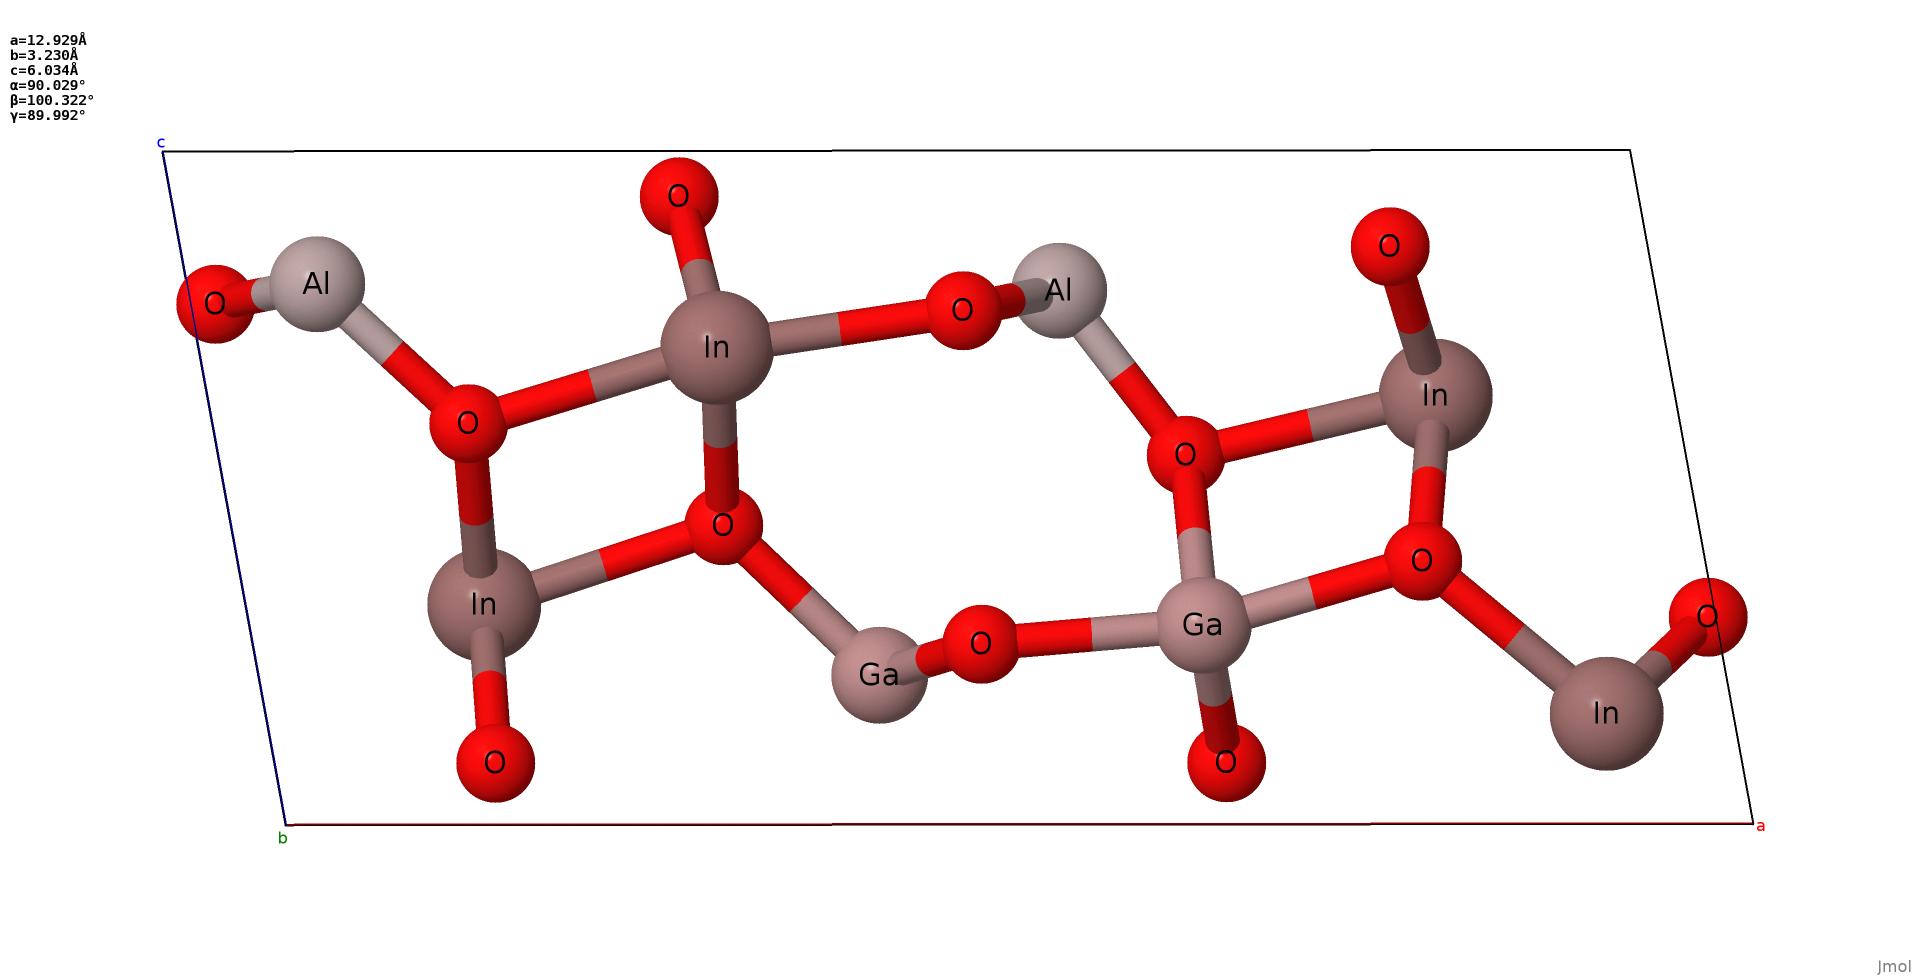
\includegraphics[scale=0.23]{train_id_20_final_hotovo.png}
	\caption{The unit cell of $(Al_{0.25}Ga_{0.25}In_{0.5})_2 O_3$ as viewed along the lattice vector $\bm{b}$ \parencite{jmol}}
	\label{example}
\end{figure}

1. The distance matrix $\bm{D}$ is calculated. If the reduced coordinates are available, the procedure follows the steps outlined in Chapter 2. If we have only the Cartesian coordinates and the lattice vectors, the reduced coordinates can be calculated as $\bm{r} = \bm{A}^{-1} \bm{R}$ for every atom in the unit cell. The corresponding distance matrix has the form (the order of the rows/columns is \ref{example} in accord with the position of the atoms tables above):

\tiny
$$\bm{D}=\begin{pmatrix}
	0 & 3.411 & 6.613 & 4.628 & 3.549 & 3.577 & 6.034 & 3.641 & 2.001 & 3.17 & 6.216 & 3.741 & 2.106 & 3.873 & 5.65 & 4.639 & 3.327 & 2.033 & 5.169 & 5.541\\
	3.411 & 0 & 4.879 & 6.59 & 3.612 & 3.53 & 3.569 & 5.945 & 3.491 & 1.785 & 3.66 & 6.448 & 4.026 & 1.815 & 4.467 & 5.718 & 1.852 & 3.422 & 5.694 & 5.51\\
	6.613 & 4.879 & 0 & 3.688 & 5.48 & 3.54 & 3.469 & 3.302 & 6.085 & 3.828 & 1.846 & 3.151 & 5.143 & 4.541 & 1.904 & 3.323 & 5.456 & 5.653 & 3.653 & 1.867\\
	4.628 & 6.59 & 3.688 & 0 & 3.441 & 5.774 & 3.456 & 3.398 & 3.351 & 6.509 & 3.449 & 1.82 & 4.305 & 5.575 & 3.61 & 1.83 & 5.5 & 5.548 & 1.834 & 3.578\\
	3.549 & 3.612 & 5.48 & 3.441 & 0 & 4.901 & 6.544 & 3.3 & 2.117 & 4.757 & 6.512 & 3.717 & 2.182 & 4.703 & 6.374 & 2.259 & 2.334 & 3.094 & 4.528 & 4.838\\
	3.577 & 3.53 & 3.54 & 5.774 & 4.901 & 0 & 3.455 & 6.536 & 5.035 & 2.139 & 3.653 & 6.54 & 4.949 & 2.27 & 2.222 & 6.322 & 3.527 & 2.149 & 5.203 & 4.682\\
	6.034 & 3.569 & 3.469 & 3.456 & 6.544 & 3.455 & 0 & 4.73 & 5.993 & 3.795 & 2.122 & 4.404 & 6.491 & 2.291 & 2.25 & 4.534 & 4.717 & 5.091 & 2.188 & 3.5\\
	3.641 & 5.945 & 3.302 & 3.398 & 3.3 & 6.536 & 4.73 & 0 & 3.717 & 6.348 & 4.437 & 2.026 & 2.013 & 6.702 & 4.603 & 2.205 & 5.349 & 4.735 & 3.328 & 1.958\\
	2.001 & 3.491 & 6.085 & 3.351 & 2.117 & 5.035 & 5.993 & 3.717 & 0 & 4.203 & 6.481 & 3.307 & 2.785 & 5.054 & 6.563 & 3.031 & 3.088 & 3.565 & 3.805 & 5.021\\
	3.17 & 1.785 & 3.828 & 6.509 & 4.757 & 2.139 & 3.795 & 6.348 & 4.203 & 0 & 3.286 & 6.638 & 5.082 & 2.999 & 3.321 & 6.799 & 2.841 & 3.047 & 5.555 & 4.406\\
	6.216 & 3.66 & 1.846 & 3.449 & 6.512 & 3.653 & 2.122 & 4.437 & 6.481 & 3.286 & 0 & 3.854 & 6.307 & 3.174 & 2.927 & 4.977 & 4.191 & 5.364 & 3.14 & 3.006\\
	3.741 & 6.448 & 3.151 & 1.82 & 3.717 & 6.54 & 4.404 & 2.026 & 3.307 & 6.638 & 3.854 & 0 & 2.949 & 6.527 & 4.896 & 2.73 & 5.45 & 4.431 & 2.824 & 2.889\\
	2.106 & 4.026 & 5.143 & 4.305 & 2.182 & 4.949 & 6.491 & 2.013 & 2.785 & 5.082 & 6.307 & 2.949 & 0 & 4.69 & 6.37 & 2.796 & 3.621 & 3.031 & 4.611 & 3.952\\
	3.873 & 1.815 & 4.541 & 5.575 & 4.703 & 2.27 & 2.291 & 6.702 & 5.054 & 2.999 & 3.174 & 6.527 & 4.69 & 0 & 2.909 & 6.529 & 2.945 & 3.094 & 4.466 & 4.918\\
	5.65 & 4.467 & 1.904 & 3.61 & 6.374 & 2.222 & 2.25 & 4.603 & 6.563 & 3.321 & 2.927 & 4.896 & 6.37 & 2.909 & 0 & 4.12 & 4.88 & 4.334 & 3.258 & 2.976\\
	4.639 & 5.718 & 3.323 & 1.83 & 2.259 & 6.322 & 4.534 & 2.205 & 3.031 & 6.799 & 4.977 & 2.73 & 2.796 & 6.529 & 4.12 & 0 & 4.584 & 4.816 & 2.844 & 2.938\\
	3.327 & 1.852 & 5.456 & 5.5 & 2.334 & 3.527 & 4.717 & 5.349 & 3.088 & 2.841 & 4.191 & 5.45 & 3.621 & 2.945 & 4.88 & 4.584 & 0 & 2.777 & 6.552 & 6.575\\
	2.033 & 3.422 & 5.653 & 5.548 & 3.094 & 2.149 & 5.091 & 4.735 & 3.565 & 3.047 & 5.364 & 4.431 & 3.031 & 3.094 & 4.334 & 4.816 & 2.777 & 0 & 6.567 & 6.607\\
	5.169 & 5.694 & 3.653 & 1.834 & 4.528 & 5.203 & 2.188 & 3.328 & 3.805 & 5.555 & 3.14 & 2.824 & 4.611 & 4.466 & 3.258 & 2.844 & 6.552 & 6.567 & 0 & 2.944\\
	5.541 & 5.51 & 1.867 & 3.578 & 4.838 & 4.682 & 3.5 & 1.958 & 5.021 & 4.406 & 3.006 & 2.889 & 3.952 & 4.918 & 2.976 & 2.938 & 6.575 & 6.607 & 2.944 & 0
\end{pmatrix}$$
\normalsize

2. The coordination of every atom $j$ is determined by the number of times the expression $$\bm{D}_{ij} < \alpha(R^S_i + R^S_j)$$ holds for all $i \neq j$ where only metal/oxygen pairs are considered. This results in the following:
\begin{table}[H]
	\tiny
	\centering
	\begin{tabular}{l|llllllllllllllllllll}
		\hline
		X-n & In-3  &Al-3  &	Ga-3 & Al-3 & In-4  & In-4  & In-4  & Ga-4  & O-2  & O-2  & O-2 & O-2 & O-3 & O-3 & O-3 & O-3 & O-2 & O-2  & O-2 & O-2   \\
		\hline
	\end{tabular}
	\caption{The atom-coordination pairs of $(Al_{0.25}Ga_{0.25}In_{0.5})_2 O_3$}
	\label{atom_coordinations}
\end{table}
We can see from the Table \ref{atom_coordinations} above the element and its amount of neighbors. For metals, the neighbors are oxygen, for oxygen, the neighbors are metals.

Now, we can generate the unigram, bigram, trigram, etc. matrix. The connections between all the atoms of the unit cell can be conveniently visualized as a graph (Figure \ref{graph}) where the nodes are atoms and edges mean the equation $\bm{D}_{ij} < \alpha(R^S_i + R^S_j)$ for two given atoms $i$ and $j$ holds.
\begin{figure}[H]
	\centering
	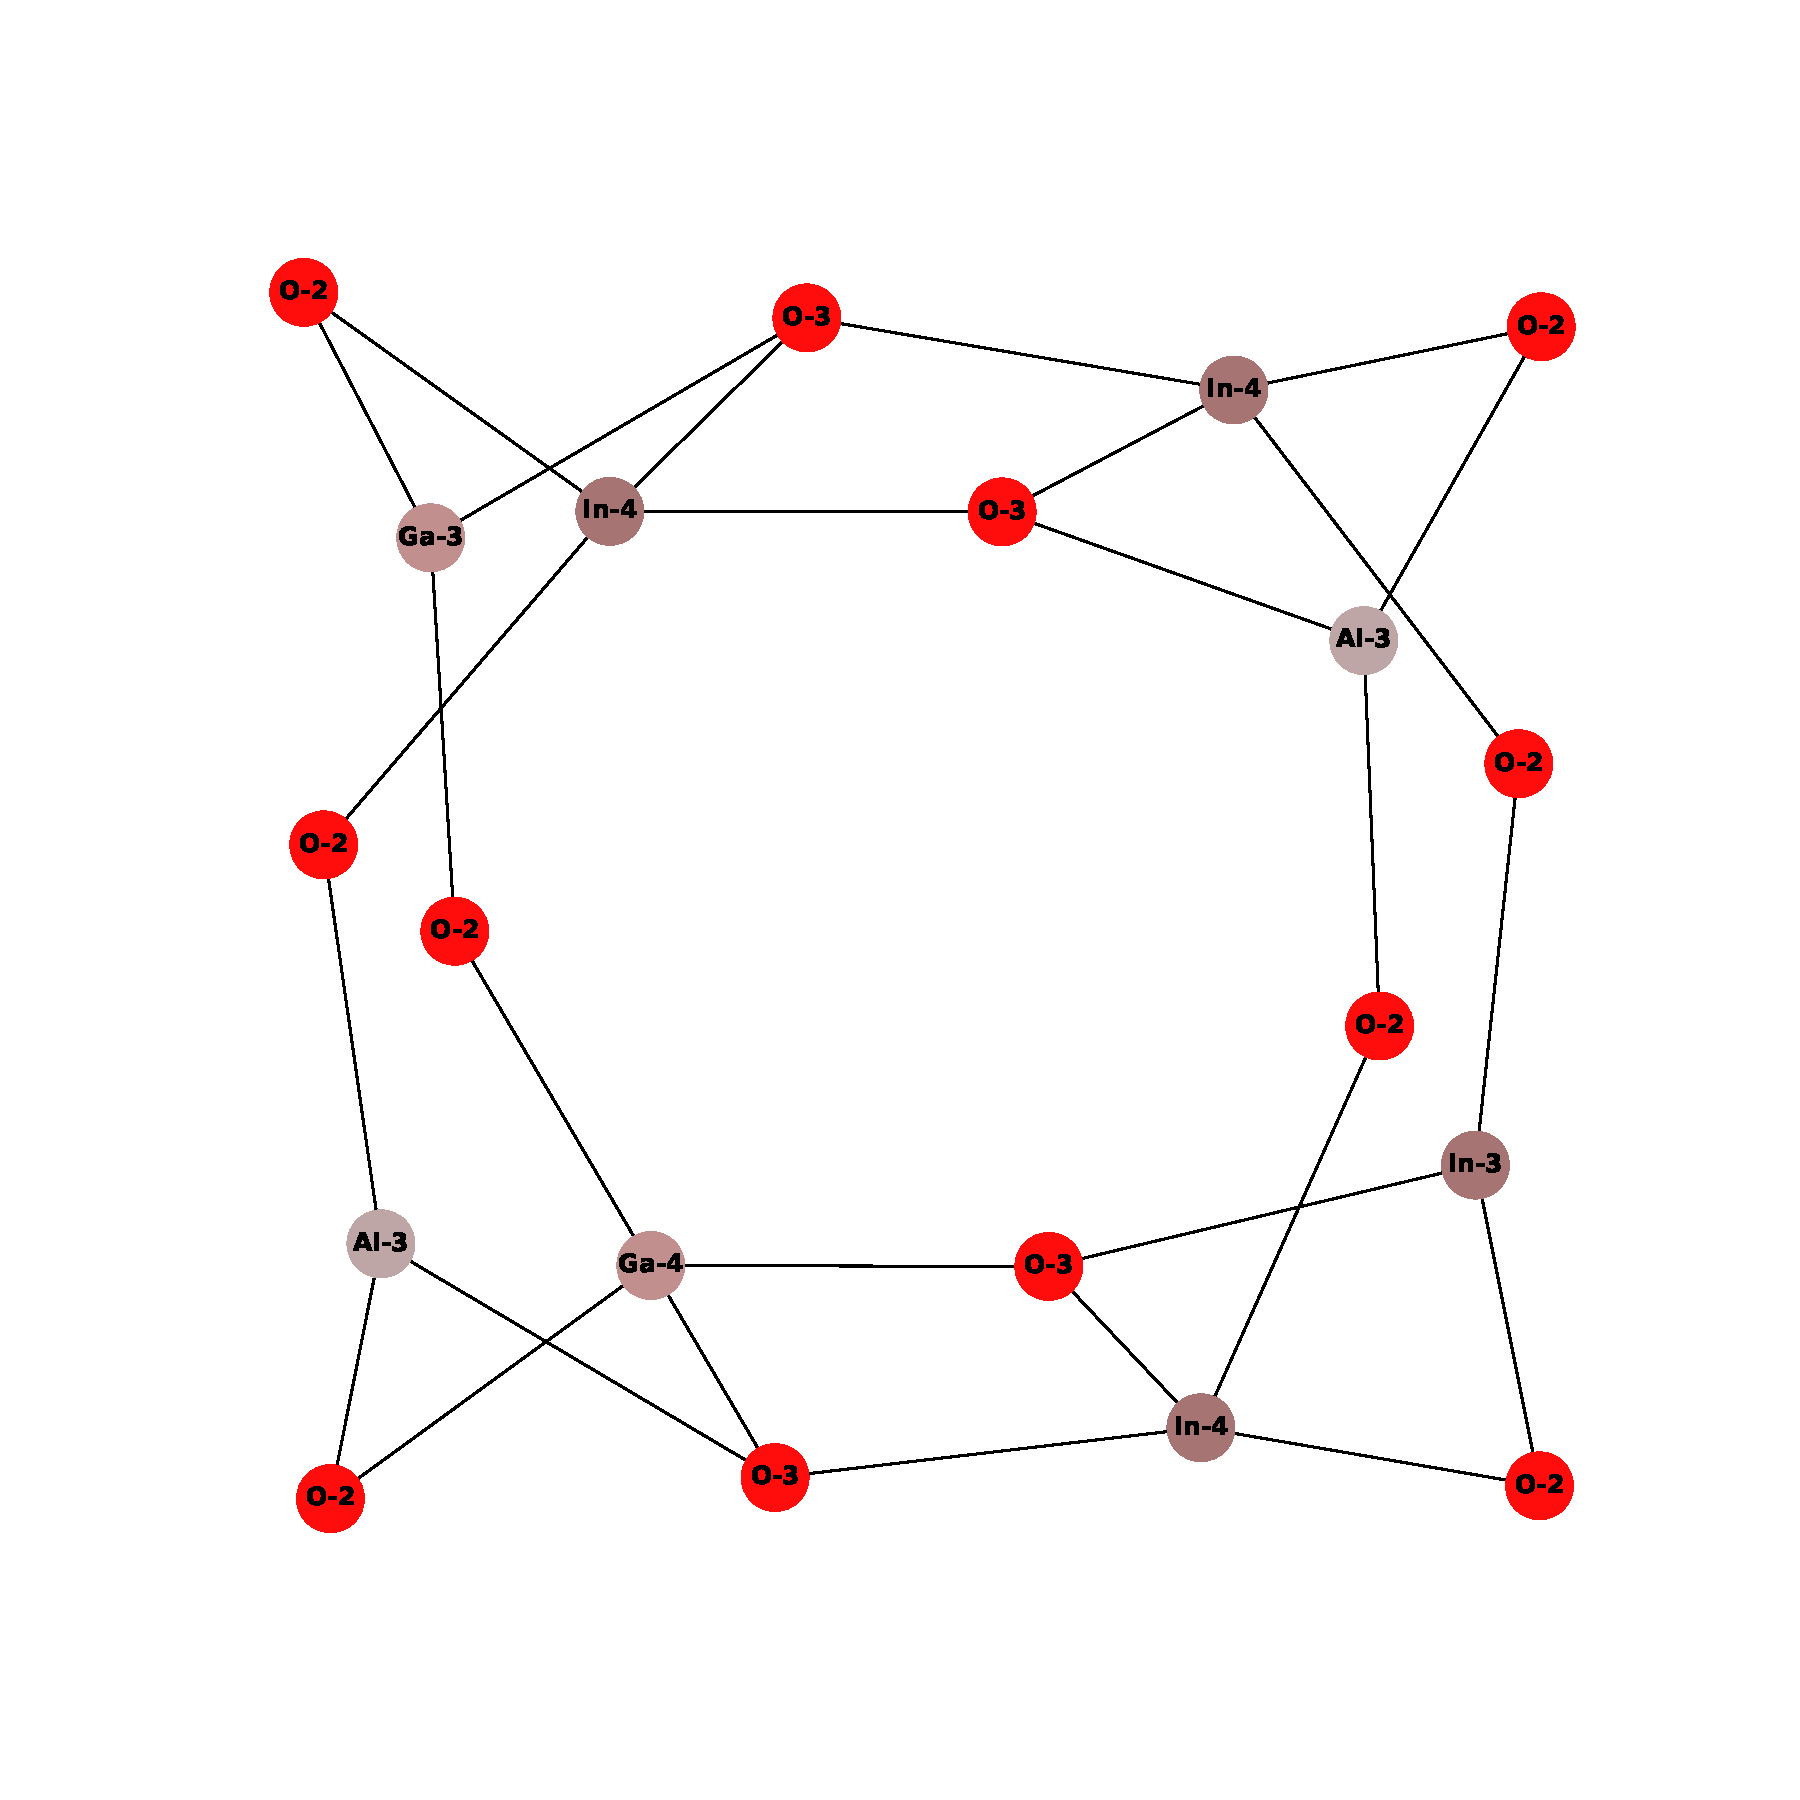
\includegraphics[scale=0.5]{id_20_graph.pdf}
	\caption{Connections between coordination environments of an alloy $(Al_{0.25}Ga_{0.25}In_{0.5})_2 O_3$ visualized as a graph \parencite{networkx}}
	\label{graph}
\end{figure}

3. To conclude the example, the unigram matrix of the material is constructed. We choose the unigram matrix because it can be easily visualized for demonstration purposes. The construction of higher order matrices is similar. We count the number of atom-coordination pairs in Table \ref{atom_coordinations} and divide each count by the volume of the unit cell $V_{cell} = \left| \det \bm{A} \right| = \left| \det \bm{(\bm{a}, \bm{b}, \bm{c})} \right| = 247.918 \, \AA^3$. The result can be seen in Figure \ref{unigram}. The reason for choosing the amount of coordinations $c = 10$ (e. g. Al-0, Al-1,..., Al-9) is that other materials in the dataset have different nonzero atom-coordination pairs and we want to include all the information into the matrix before we leave out any columns either for the reason of reducing the size of the matrix or simply because some columns are only zeros for all materials in the dataset.

\begin{figure}[H]
	\centering
	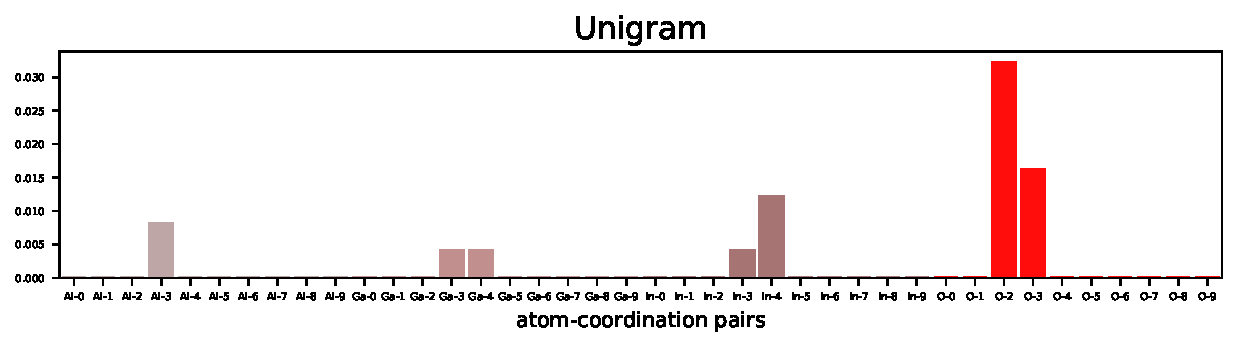
\includegraphics[scale=.85]{unigram_id_20.pdf}
	\caption{Unigram of an alloy $(Al_{0.25}Ga_{0.25}In_{0.5})_2 O_3$}
	\label{unigram}
\end{figure}
Naturally, the bigram descriptor would be constructed by counting the number of pairs of atom-coordinations present in the graph. The trigram would be contructed by counting the number of triplets of atom-coordinations present in the graph, etc. This marks the end of the example.

\chapter{Implementation and Attached Storage Device}
\printbibliography
\end{document}

The unigram, bigram, trigram and quadgram descriptors were tested on the final, Vegard and relaxation datasets. The relaxation dataset predicts energies for the 600 final datapoints in final and Vegard test set but also their relaxations which means total of 6832 test datapoints which means roughly the same test-train split as for the final and Vegard datasets. The hyperparameters were optimized on a logarithmic grid using grid search and 5-fold cross validation. The results are in the following tables:

\begin{table}[H]
	\centering
	\begin{tabular}{lllll} 
		\hline
		RMSE                        & in eV     & 1-g   & 2-g   & 3-g    \\ 
		\hline
		\multirow{2}{*}{Final}      & Formation & 0.032 & 0.029 & 0.029  \\
		& Bandgap   & 0.202 & 0.199 & 0.174  \\ 
		\hline
		\multirow{2}{*}{Vegard}     & Formation & 0.026 & 0.025 & 0.027  \\
		& Bandgap   & 0.192 & 0.195 & 0.186  \\ 
		\hline
		\multirow{2}{*}{Relaxation} & Formation & 0.031 & 0.030 & 0.028  \\
		& Bandgap   & 0.210 & 0.204 & 0.210 \\
		\hline
	\end{tabular}
	\caption{ unigram (1-g), bigram (2-g), trigram (3-g) RMSE test error}
\end{table}

\begin{table}[H]
	\centering
	\begin{tabular}{lllll} 
		\hline
		MAE                       & in eV     & 1-g   & 2-g   & 3-g    \\ 
		\hline
		\multirow{2}{*}{Final}      & Formation & 0.018 & 0.016 & 0.015  \\
		& Bandgap   & 0.112 & 0.110 & 0.098  \\ 
		\hline
		\multirow{2}{*}{Vegard}     & Formation & 0.015 & 0.014 & 0.015  \\
		& Bandgap   & 0.112 & 0.115 & 0.110  \\ 
		\hline
		\multirow{2}{*}{Relaxation} & Formation & 0.118 & 0.118 & 0.017  \\
		& Bandgap   & 0.122 & 0.120 & 0.119 \\
		\hline
	\end{tabular}
	\caption{ unigram (1-g), bigram (2-g), trigram (3-g) MAE test error}
\end{table}

\begin{table}[H]
	\centering
	\begin{tabular}{lllll} 
		\hline
		RMSLE                       & in eV     & 1-g   & 2-g   & 3-g    \\ 
		\hline
		\multirow{2}{*}{Final}      & Formation & 0.024 & 0.022 & 0.022  \\
		& Bandgap   & 0.097 & 0.091 & 0.086  \\ 
		\hline
		\multirow{2}{*}{Vegard}     & Formation & 0.021 & 0.020 & 0.021  \\
		& Bandgap   & 0.089 & 0.089 & 0.085  \\ 
		\hline
		\multirow{2}{*}{Relaxation} & Formation & 0.024 & 0.023 & 0.023  \\
		& Bandgap   & 0.090 & 0.089 & 0.085 \\
		\hline
	\end{tabular}
	\caption{ unigram (1-g), bigram (2-g), trigram (3-g) RMSLE test error}
\end{table}

We can see that the relaxation dataset does not perform better than the rest even though its computational demand is much greater. For comparison, the competition values of unigram, bigram and trigram RMSLE errors:

\begin{table}[H]
	\centering
	\begin{tabular}{lllll} 
		\hline
		RMSLE                   & in eV     & 1-g   & 2-g   & 3-g    \\ 
		\hline
		\multirow{2}{*}{Vegard} & Formation & 0.023 & 0.023 & 0.022  \\
		& Bandgap   & 0.082 & 0.081 & 0.081  \\
		\hline
	\end{tabular}
	\caption{Competition RMSLE for Vegard dataset \parencite{sutton19}}
\end{table}
Our model performs better for formation energy but worse for bandgap energy. This is a trend which was observed with our model. The hyperparameter optimization also influences each of the energies differently and slight overfitting or underfitting could play a role here.

We test our proposed ngram extension of equation (\ref{proposed}) in the final dataset with the unigram represenation. We employed the following procedure: we start with $p=0$, then we tested $p \in \{ -1, 0, 1\}$ , then $p \in \{-2, -1, 0, 1, 2\}$, and so on until we reach $p \in \{-12, \dots, 12\}$. This bound was chosen in this way, because functions of interatomic distances of form $\frac{1}{r^n}$ for some value of $n \in \mathbb{N}$ model well interatomic potentials in crystals \parencite{kraus16}. Figure \ref{p} shows the results.
\begin{table}[H]
	\centering
	\begin{tabular}{llccc} 
		\hline
		In eV 	&     &  $p=0$    & $p \in \{-1, 0, 1\}$       &  $p \in \{-12, \dots, 12\}$      \\ 
		\hline
		\multirow{2}{*}{RMSE}  & Formation & 0.029 & 0.016 & 0.035  \\
		& Bandgap   & 0.220 & 0.202 & 0.240  \\ 
		\hline
		\multirow{2}{*}{RMSLE} & Formation & 0.023 & 0.013 & 0.027  \\
		& Bandgap   & 0.100 & 0.091 & 0.107  \\ 
		\hline
		\multirow{2}{*}{MAE}   & Formation & 0.018 & 0.009 & 0.021  \\
		& Bandgap   & 0.123 & 0.115 & 0.140  \\
		\hline
	\end{tabular}
	\caption{Changes in predicted energy based on $p$.}
	\label{p}
\end{table}
We report only up to to $p \in \{ -1, 0, 1\}$ because the error starts to rise afterwards up until $p \in \{-12, \dots, 12\}$. This could mean bad overfitting in the sense the amount of terms of $\frac{1}{r^n}$ and ${r^n}$. The best result is with the simplest model which includes the average bond distances of (\ref{proposed}). Overall, this model greatly improves the ngram descriptor and has the ability to tune its complexity in similar fashion with the parameter $p$.
